\documentclass[11pt]{amsart}
\usepackage{amsmath,amssymb,amsthm}
\usepackage{booktabs}
\usepackage{float}
\usepackage{tikz}
\usetikzlibrary{positioning,arrows.meta,calc}
\usepackage[margin=1.1in]{geometry}
\usepackage[colorlinks=true,linkcolor=blue,citecolor=blue,urlcolor=blue]{hyperref}

\newtheorem{theorem}{Theorem}[section]
\newtheorem{lemma}[theorem]{Lemma}
\newtheorem{proposition}[theorem]{Proposition}
\newtheorem{corollary}[theorem]{Corollary}
\newtheorem{conjecture}[theorem]{Conjecture}
\newtheorem*{theoremB}{Theorem B}
\newtheorem*{theoremC}{Theorem C}
\newtheorem*{theoremA}{Theorem A}
\theoremstyle{definition}
\newtheorem{definition}[theorem]{Definition}
\newtheorem{hypothesis}[theorem]{Hypothesis}
\theoremstyle{remark}
\newtheorem{remark}[theorem]{Remark}

\newcommand{\N}{\mathbb{N}}
\newcommand{\Z}{\mathbb{Z}}
\newcommand{\PP}{\mathbb{P}}
\newcommand{\Lflat}{\Lambda_2^{\flat}}
\newcommand{\res}{\mathrm{res}}
\newcommand{\capR}{\mathrm{cap}}
\newcommand{\TODO}[1]{\textbf{[TODO: #1]}}

\title[Dilation methods and the twin prime parity barrier]{Why expansion methods for Chowla do not reach twin primes:\\ a method-limitation theorem and an explicit parity compiler}
\author{Liang Wang}
\address{School of Artificial Intelligence and Automation, Huazhong University of Science and Technology, Wuhan 430070, P.R. China}
\email{wangliang.f@gmail.com}
\date{Draft v1.3, 29 October 2026}
\raggedbottom

\begin{document}
\begin{abstract}
The logarithmically averaged two-point Chowla conjecture was proved by Tao and quantitatively improved by Helfgott--Radziwi\l{}\l{} and Pilatte. The mechanism is a dilation identity followed by a spectral bound for a divisibility operator. On the generalised Elliott--Halberstam conjecture (GEH), Bombieri's asymptotic sieve turns the twin prime conjecture into a Chowla-type statement on almost primes. Tao remarked that the restriction to almost primes destroys the multiplicativity on which the Chowla arguments rely. We make this remark into a theorem. We define a class of dilation--spectral certificates that contains the Helfgott--Radziwi\l{}\l{} and Pilatte certificates adapted to the shift $2$, and allows arbitrary smooth, rough or mixed dilators up to $x^{\kappa}$. We prove that the resolution of every such certificate on twin-type parity is $\gg\eta\min(1,\eta/\kappa)\log x$, where $x^\eta$ is the roughness level. So these certificates cannot even exclude the extreme parity configuration that would kill twin primes. The proof uses only one edge of the divisibility graph and two sieve bounds. It shows that the loss comes from the factor $1/\log x^\eta$ that two-sided roughness costs on every edge, a loss that no choice of weights or spectral bound can recover. To state precisely what such a certificate would have to resolve, we write the Bombieri--Tao reformulation as an exact, numerically testable identity. With $\Lflat=\mu^2\Lambda_2$,
\[
\sum_{n\le X}\frac{\Lambda(n)\Lambda(n+2)}{n}=\tfrac14\mathcal M(X)\bigl(1+\rho(X)\bigr)+O(1),
\]
where $\rho(X)$ is an explicit logarithmic parity defect of the Liouville function on almost-prime pairs, and $\mathcal M(X)\sim8\Pi_2\log X$ on GEH. We also show, via Bombieri's one-sided theorem applied on both sides, that the joint parity of rough pairs is governed by the twin parameter alone. Consequently a single class of rough pairs suffices, for instance a positive proportion of pairs of rough products of two primes, and for that class we give a quantitative form that uses only Bombieri's theorem. Finally we connect the Chowla and twin endpoints by the family of completely multiplicative functions $g_t$ with $g_t(p)=t$ below the roughness level, and prove that dilation--spectral certificates, in $\ell^2$ or any $\ell^p$ norm and with arbitrary nonnegative weights, cannot reach damping $|t|<0.676$. Reading the Polymath8b proof of $H_1\le6$ in the same language, we show that GEH together with a single comparison between the masses of twin pairs and of gap-$4$ and gap-$6$ pairs implies the twin prime conjecture. Finally we locate the barrier along the remaining coordinates. On GEH the gaps occurring infinitely often have density at least $\frac16$, and a counterfeit modulo $3$ shows this is sharp for sieve methods. A census of known parity-breaking results shows that each ends in a bilinear form $\sum a_mb_n\,c(mn)$ whose cancellation comes from structure in $c$. For twins $c=\lambda(\cdot+2)$, and we prove that every argument that uses only absolute values of the associated Dirichlet polynomials (in the Bohr mean) stays a constant factor from the trivial bound. Nothing here proves or disproves the twin prime conjecture.
\end{abstract}
\maketitle
\tableofcontents

%======================================================================
\section{Introduction}\label{sec:intro}
%======================================================================

\subsection{The question}
Let $\lambda(n)=(-1)^{\Omega(n)}$ be the Liouville function and $\Pi_2=\prod_{p>2}(1-(p-1)^{-2})$. Two parity problems sit side by side.
\begin{itemize}
\item The two-point Chowla conjecture $\sum_{n\le x}\lambda(n)\lambda(n+1)=o(x)$ is open. Its logarithmic average was proved by Tao \cite{Tao16}; a proof of the ordinary average has been claimed in a 2026 AI-generated preprint that has not been refereed \cite{OpenAI26}. Helfgott and Radziwi\l{}\l{} \cite{HR21} then obtained the bound $O(\log x/(\log\log x)^{1/2})$ for $\sum_{n\le x}\lambda(n)\lambda(n+1)/n$, and Pilatte \cite{Pil23} the bound $O((\log x)^{1-c})$.
\item The twin prime conjecture is open. By Bombieri's asymptotic sieve \cite{Bom76,FI78}, on the Elliott--Halberstam conjectures all twin-type distribution information is determined except for one scalar $\delta_x\in[0,2]$. The twin prime conjecture follows from $\liminf\delta_x>0$, and no bound beyond $0\le\delta_x\le2$ is known even on GRH, GUE, abc and Chowla \cite{Tao16notes}.
\end{itemize}
Tao observed that, on GEH, the twin prime conjecture can be viewed ``as a sort of Chowla conjecture restricted to almost primes''. He also remarked that the recent Chowla progress relies heavily on the multiplicativity of $\mu$ at small primes, which inserting a roughness weight $1_R$ completely destroys \cite{Tao16notes}. This paper asks whether that remark can be made precise. Can the expansion mechanism of \cite{HR21,Pil23}, which is formulated for arbitrary $1$-bounded functions once the dilation identity has been applied, be adapted to the twin problem? Or is there a structural reason why it cannot? Figure~\ref{fig:roadmap} summarises the answer and the logical structure of the paper.

% Road map of the paper (Figure 1). Included from main.tex.
\begin{figure}[t]
\centering
\resizebox{\textwidth}{!}{%
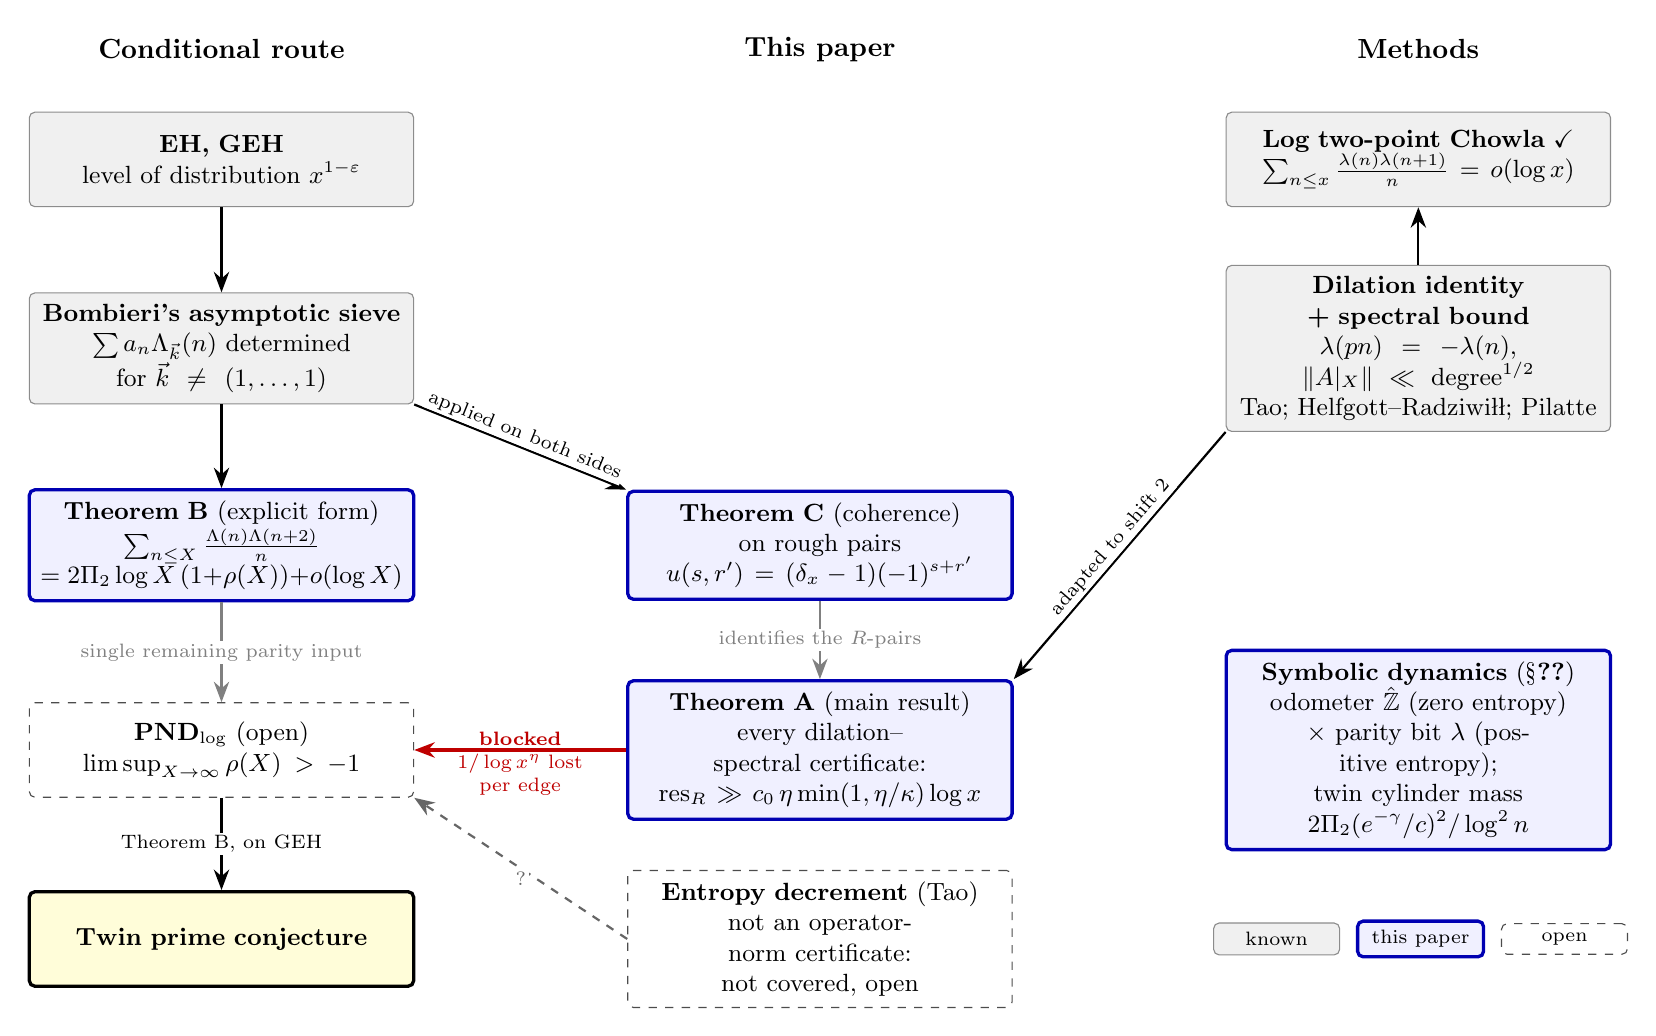
\begin{tikzpicture}[
  font=\small,
  box/.style={rounded corners=2pt,align=center,inner sep=4pt,text width=4.6cm,minimum height=1.2cm},
  known/.style={box,draw=black!45,fill=black!6},
  new/.style={box,draw=blue!70!black,very thick,fill=blue!6},
  open/.style={box,draw=black!70,dashed},
  goal/.style={box,draw=black,very thick,fill=yellow!15},
  arr/.style={-{Stealth[length=2.6mm]},thick},
  darr/.style={-{Stealth[length=2.6mm]},thick,dashed,black!60},
  lab/.style={font=\scriptsize,align=center,fill=white,inner sep=1pt}
]
% column headers
\node[font=\bfseries] at (0,1.4) {Conditional route};
\node[font=\bfseries] at (7.6,1.4) {This paper};
\node[font=\bfseries] at (15.2,1.4) {Methods};

% ---------------- left column: the conditional route ----------------
\node[known] (geh)  at (0,0)    {\textbf{EH, GEH}\\ level of distribution $x^{1-\varepsilon}$};
\node[known] (bomb) at (0,-2.4) {\textbf{Bombieri's asymptotic sieve}\\ $\sum a_n\Lambda_{\vec k}(n)$ determined\\ for $\vec k\ne(1,\dots,1)$};
\node[new]   (thmB) at (0,-4.9) {\textbf{Theorem B} (explicit form)\\ $\sum_{n\le X}\frac{\Lambda(n)\Lambda(n+2)}{n}$\\ $=2\Pi_2\log X\,(1+\rho(X))+o(\log X)$};
\node[open]  (pnd)  at (0,-7.5) {\textbf{PND$_{\log}$} (open)\\ $\limsup_{X\to\infty}\rho(X)>-1$};
\node[goal]  (tpc)  at (0,-9.9) {\textbf{Twin prime conjecture}};

\draw[arr] (geh) -- (bomb);
\draw[arr] (bomb) -- (thmB);
\draw[arr,black!50] (thmB) -- node[lab]{single remaining parity input} (pnd);
\draw[arr] (pnd) -- node[lab]{Theorem B, on GEH} (tpc);

% ---------------- middle column: results of this paper ----------------
\node[new]  (thmC) at (7.6,-4.9) {\textbf{Theorem C} (coherence)\\ on rough pairs\\ $u(s,r')=(\delta_x-1)(-1)^{s+r'}$};
\node[new]  (thmA) at (7.6,-7.5) {\textbf{Theorem A} (main result)\\ every dilation--spectral certificate:\\ $\mathrm{res}_R\gg c_0\,\eta\min(1,\eta/\kappa)\log x$};
\node[open] (entr) at (7.6,-9.9) {\textbf{Entropy decrement} (Tao)\\ not an operator-norm certificate:\\ not covered, open};

\draw[arr] (bomb.south east) -- node[lab,sloped,above]{applied on both sides} (thmC.north west);
\draw[arr,black!50] (thmC) -- node[lab]{identifies the $R$-pairs} (thmA);

% barrier
\draw[arr,red!75!black,very thick] (thmA.west) -- node[lab,above,text=red!75!black]{\textbf{blocked}} node[lab,below]{$1/\log x^\eta$ lost\\ per edge} (pnd.east);
\draw[darr] (entr.west) -- node[lab,below]{?} (pnd.south east);

% ---------------- right column: the methods ----------------
\node[known] (chow) at (15.2,0)    {\textbf{Log two-point Chowla} \checkmark\\ $\sum_{n\le x}\frac{\lambda(n)\lambda(n+1)}{n}=o(\log x)$};
\node[known] (mech) at (15.2,-2.4) {\textbf{Dilation identity + spectral bound}\\ $\lambda(pn)=-\lambda(n)$, $\ \|A|_X\|\ll\text{degree}^{1/2}$\\ Tao; Helfgott--Radziwi\l{}\l{}; Pilatte};
\node[new]   (dyn)  at (15.2,-7.5) {\textbf{Symbolic dynamics} (\S\ref{sec:dynamics})\\ odometer $\hat{\mathbb Z}$ (zero entropy)\\ $\times$ parity bit $\lambda$ (positive entropy);\\ twin cylinder mass $2\Pi_2(e^{-\gamma}/c)^2/\log^2n$};

\draw[arr] (mech) -- (chow);
\draw[arr] (mech.south west) -- node[lab,sloped,above]{adapted to shift 2} (thmA.north east);

% ---------------- legend ----------------
\node[draw=black!45,fill=black!6,rounded corners=2pt,font=\scriptsize,minimum width=1.6cm] (l1) at (13.4,-9.9) {known};
\node[draw=blue!70!black,very thick,fill=blue!6,rounded corners=2pt,font=\scriptsize,minimum width=1.6cm,right=2mm of l1] (l2) {this paper};
\node[draw=black!70,dashed,rounded corners=2pt,font=\scriptsize,minimum width=1.6cm,right=2mm of l2] {open};
\end{tikzpicture}}
\caption{Road map. Left: the conditional route. On GEH, Bombieri's sieve and Theorem~B reduce the twin prime conjecture to the single parity input PND$_{\log}$, and Theorem~C shows that on rough pairs this input is the only parity parameter. Right: the dilation--spectral mechanism that proved logarithmic Chowla. Theorem~A shows that, adapted to twin primes, it cannot resolve this parity input, because two-sided roughness costs a factor $1/\log x^\eta$ on every edge. Entropy decrement is the one successful mechanism not covered. Bottom right: the symbolic-dynamics picture behind the paper (Proposition~\ref{prop:coupling}).}
\label{fig:roadmap}
\end{figure}


\subsection{The mechanism}
Tao's reduction \cite{Tao16} uses $\lambda(pn)=-\lambda(n)$ to replace the correlation $\sum_n\lambda(n)\lambda(n+1)/n$ by an average over dilators $d$ of
\[
\sum_{\substack{n\\ d\mid n}}\lambda(n)\lambda(n+d).
\]
Helfgott and Radziwi\l{}\l{} compare this with the ``random'' sum $\sum_nd^{-1}\lambda(n)\lambda(n+d)$, which is controlled by the Matomäki--Radziwi\l{}\l{} theorem \cite{MR16}. The difference is a quadratic form $\langle\lambda,A\lambda\rangle$ for a divisibility operator $A$. Its norm, after restriction to a dense set, is $O(\sqrt L)$ for prime dilators with $L=\sum1/p$ \cite{HR21}, and $e^{O(J)}V^{J/2}$ for products of $J$ primes \cite{Pil23}, against the trivial bounds $L$ and $V^J$. The saving of a square root of the degree is what proves logarithmic Chowla.

For twin primes the analogous target is the parity correlation on pairs $(m,m+2)$ with both entries $x^\eta$-rough; Theorem~C below shows that this is where the twin parameter lives. A dilation $d$ sends such a pair to the edge $(dm,d(m+2))$. The $R$-capacity $\capR_R$ is the trivial bound for the part of the quadratic form coming from such edges. A certificate determines the normalised twin correlation, which lies in $[-1,1]$, only up to $\pm\res_R$, where
\[
\res_R=\frac{\|A\|\,\|f\|_2\|g\|_2}{\capR_R}
\]
is its \emph{resolution} (Definition~\ref{def:cert}).

\subsection{Main result}
\begin{theoremA}[Limits of dilation--spectral certificates]
Let $0<\eta\le1/10$, $z=x^\eta$ and $0<\kappa\le1-4\eta$. Every dilation--spectral certificate in the sense of Definition~\ref{def:cert} satisfies
\[
\res_R\ \ge\ c\,c_0\,\eta\min\Bigl(1,\frac\eta\kappa\Bigr)\log x,
\]
where $c>0$ is absolute and $c_0$ is the lower bound for the divisibility coefficients. The certificate may have arbitrary dilators in $[2,x^\kappa]$ (smooth, rough or mixed $d=st$), arbitrary weights, multiplicative $1$-bounded functions, and an arbitrary restriction set retaining half of the relevant closure set. The class contains the certificates of Helfgott--Radziwi\l{}\l{} and Pilatte adapted to the shift $2$ (Table~\ref{tab:certs}, Remark~\ref{rem:check}). In particular, no such certificate can establish $\limsup\rho>-1$ in Theorem~B, which on GEH is the input the twin prime conjecture needs.
\end{theoremA}

The proof (Section~\ref{sec:limits}) is short and uses neither the specific spectral bounds nor any information about $\lambda$. A single divisibility edge forces $\|A\|\ge c_0\max w_d$, so the weights cancel. Multiplicativity of $f,g$ forces them to be unimodular on a set $\mathcal K$ of size $\asymp x(1+V_s)/\log z$. An upper bound sieve of dimension $2$ bounds the number of $R$-pair edges by $\ll xV/\log^2z$. The extra factor $1/\log z$, the probability that $m+2$ is also rough, is paid on every edge, and grouping the dilators by their smooth part makes the bound uniform in $D$. When $z=O(1)$ (the Chowla setting) the bound degenerates, consistent with \cite{Tao16,HR21,Pil23}. We also explain why the obvious escape, building the pair condition into $f$ and $g$, makes the comparison term itself a twin-type correlation, so that the method becomes circular.

\subsection{What the certificate would have to resolve}
To make the target precise, we write the Bombieri--Tao reformulation as an exact identity. Let $\Lambda_2=\mu*\log^2$ and $\Lflat=\mu^2\Lambda_2$; thus $\Lflat(p)=\log^2p$, $\Lflat(pq)=2\log p\log q$ for primes $p\ne q$, and $\Lflat=0$ otherwise. Let $w(n)=1/(n\log n\log(n+2))$ and
\[
\mathcal M(X)=\sum_{3\le n\le X}\Lflat(n)\Lflat(n+2)w(n),\qquad
\mathcal D(X)=\sum_{3\le n\le X}\Lflat(n)\Lflat(n+2)\bigl(\lambda(n)\lambda(n+2)-\lambda(n)-\lambda(n+2)\bigr)w(n),
\]
and $\rho(X)=\mathcal D(X)/\mathcal M(X)$. Note $\rho(X)\ge-1$, with equality iff no twin prime pair lies in $[3,X]$.

\begin{theoremB}[Explicit Bombieri--Tao form]
Unconditionally,
\[
\sum_{n\le X}\frac{\Lambda(n)\Lambda(n+2)}{n}=\tfrac14\mathcal M(X)\bigl(1+\rho(X)\bigr)+O(1).
\]
On EH and GEH, $\mathcal M(X)=(8\Pi_2+o(1))\log X$, so that
\[
\sum_{n\le X}\frac{\Lambda(n)\Lambda(n+2)}{n}=2\Pi_2\log X\,(1+\rho(X))+o(\log X).
\]
In particular, on EH and GEH, if $\limsup_{X\to\infty}\rho(X)>-1$ there are infinitely many twin primes.
\end{theoremB}

The defect splits as $\rho=(\bar\delta^{(1)}-1)+(\bar\delta^{(2)}-1)+\rho_3$. Here $\bar\delta^{(j)}$ are logarithmic versions of Bombieri's two one-sided parity parameters, and $\rho_3$ is the two-point correlation of $\lambda$ on almost-prime pairs (Remark~\ref{rem:split}). In particular the one-point terms are \emph{not} negligible: they carry the one-sided Bombieri parameters. On the rough pairs that Theorem~A concerns, the parity structure is one-dimensional.

\begin{theoremC}[Coherence of two-sided parity]
Assume EH and GEH. Let $u(s,r')$ be the relative deviation, from the product model $2\Pi_2\nu_s\nu_{r'}x/\log^2x$, of the number of squarefree $x^\eta$-rough pairs $(m,m+2)$ with $\omega(m)=s$ and $\omega(m+2)=r'$. Then $u(s,r')=(\delta_x-1)(-1)^{s+r'}+o(1)$, where $\delta_x$ is the twin parity parameter.
\end{theoremC}

Theorem~C follows by applying Bombieri's one-sided theorem (Theorem~\ref{thm:onesided}, for which we include a self-contained proof) to sequences supported on both sides of the pair. It justifies the choice of $R$-pairs in Theorem~A. On rough pairs the twin parameter $\delta_x$ is the only parity parameter; pairs with a non-rough entry carry a priori different parameters.

\subsection{Further results}
\begin{itemize}
\item \emph{The roughness ceiling of known mechanisms} (Section~\ref{sec:ceiling}, Table~\ref{tab:ceiling}). Theorem~A holds uniformly in the roughness level $z$. Consequently, dilation--spectral certificates can resolve parity only on $z$-rough integers with $z\le\exp(O(\sqrt{\log x}))$ (Corollary~\ref{cor:ceiling}, a theorem). Theorem~E proves the analogous limitation for entropy-decrement certificates, the class containing Tao's argument and its variance-sensitive variants: their reach is $z\le(\log x)^{O(\varepsilon^4)}$ at precision $\varepsilon$. We also analyse the recent argument of Lü--Wang--Wu for $\mu(p+2)$ \cite{LWW26}, which reaches $z\le\exp((\log x)^c)$ with $c<\frac15$. That analysis concerns their specific proof, not every argument of its kind. All known mechanisms stop far below the roughness $x^\eta$ that Bombieri's parameter requires.
\item \emph{Equivalent targets} (Section~\ref{sec:targets}). On GEH, any single class of rough pairs determines $\delta_x$: an even class through a lower bound, an odd class through an upper bound below twice the product model (Corollary~\ref{cor:anyclass}). For pairs of rough products of two primes, Proposition~\ref{prop:Q} gives the relation with twin primes using only Bombieri's theorem, with error $O(\eta+\varepsilon(x)+1/\log x)$ relative to $x\log^2x$, so that the required proportion is quantified (Corollary~\ref{cor:Q}).
\item \emph{Shifts and the Polymath8b disjunction} (Section~\ref{sec:shifts}). Theorem~C holds for the shifts $2$, $4$ and $6$ separately (Proposition~\ref{prop:shifts}), but GEH does not link the three parameters. The proof of $H_1\le6$ on GEH \cite{Polymath8b} gives a weighted disjunction between the three pair types (Proposition~\ref{prop:disjunction}), so GEH together with one comparison inequality between pair masses implies the twin prime conjecture (Theorem~\ref{thm:SC}). That inequality is exactly what the parity argument of \cite[\S8]{Polymath8b} rules out for sieve methods.
\item \emph{No derivative lines over $\mathbb Z$} (Proposition~\ref{prop:noderiv}). The mechanism behind the function-field twin prime theorem \cite{SS22} rests on a derivation; $\mathbb Z$ has none, local substitutes give periodic functions orthogonal to $\lambda$, and permutation-sign discriminants are Jacobi symbols.
\item \emph{The $t$-family ceiling} (Propositions~\ref{prop:T}, \ref{prop:L}). The completely multiplicative functions $g_t$ with $g_t(p)=t$ for $p<z$ and $g_t(p)=-1$ for $p\ge z$ interpolate between $\lambda$ ($t=-1$), Teräväinen's truncated Liouville function ($t=1$) and the twin parity ($t=0$). Dilation--spectral certificates with arbitrary nonnegative weights have $t$-resolution $\gg(\log z)^{(1-|t|)^2-t^4/2}$, so they fail for $|t|<0.676$, and replacing $\ell^2$ by $\ell^p$ never helps.
\item \emph{Locating the barrier} (Section~\ref{sec:locate}, Table~\ref{tab:coords}).
\begin{itemize}
\item On GEH the de Polignac numbers have lower density at least $\frac16$ (Proposition~\ref{prop:S1}), and a counterfeit modulo $3$ shows that sieve methods cannot do better, nor prove ``almost all gaps $h\le H$'' for any $H$ (Remark~\ref{rem:S2}).
\item In the proof of Matomäki--Radziwi\l{}\l{}--Tao the exponent $8/33$ comes from a spacing step in the Type $d_3$ sums. The Jutila half of that step is already optimal, and improving the $d_3$ step alone cannot go below $3/13$ (Remark~\ref{rem:MRT}).
\item A census of known parity-breaking results sorts their parity information into seven sources (Table~\ref{tab:census}), none of which applies to twins. All of them end in a bilinear form $\sum a_mb_nc(mn)$ whose cancellation comes from structure in $c$; for twins $c=\lambda(\cdot+2)$.
\item For that form, Type~I sums are easy (Remark~\ref{rem:typeI}), seven quick structural tests are null (Remark~\ref{rem:cards}), and every argument that uses only absolute values of the Dirichlet polynomials in the Bohr mean stays a constant factor from the trivial bound (Proposition~\ref{prop:absbarrier}; numerically the factor is about $0.6$). So the missing input is phase information, not a large-values estimate.
\end{itemize}
\item \emph{A parameter-free coupling law} (Proposition~\ref{prop:coupling}). In the symbolic-dynamics model of \cite{Wan26}, the fitted coupling constant $k\approx12.73$ can be eliminated. On the odometer $\hat\Z$ the Haar mass of the twin cylinder is $2\Pi_2(e^{-\gamma}/c)^2(\log n)^{-2}$ for the cutoff $n^c$. This gives the Hardy--Littlewood density exactly at Pólya's cutoff $c=e^{-\gamma}$.
\item \emph{Numerics} (Section~\ref{sec:numerics}).
\begin{itemize}
\item The two-point part $\rho_3(X)$ increases monotonically from $-0.020$ to $-0.0065$ for $X=10^4,\dots,10^7$.
\item On rough pairs the fitted coherent coefficient $\delta_x-1$ is zero within $\pm0.003$.
\item The constants of the sieve bounds behind Theorem~A are stable at $x=10^7$.
\end{itemize}
Since Theorem~B is an identity, numerical evidence for $\rho\to0$ is evidence for the Hardy--Littlewood asymptotic itself, not independent support.
\end{itemize}

\subsection{What is new and what is not}
The following are known:
\begin{itemize}
\item the parity criterion ``$\delta$ bounded below $\Rightarrow$ twin primes'', and the one-sided parity structure for general sequences (Theorem~\ref{thm:onesided}) \cite{Bom76,FI78,Tao16notes};
\item the reading of the twin prime conjecture on GEH as a Chowla conjecture on almost primes, with the Hardy--Littlewood asymptotic equivalent to $\sum\mu1_R(n)\mu1_R(n+2)=o(x/\log^2x)$, and the heuristic obstruction from the loss of multiplicativity \cite{Tao16notes};
\item the normalisation by Pólya's cutoff \cite{HL23,Pol59,MW06,BFT23}.
\end{itemize}
Related conditional approaches through one-sided parity information include \cite{MV17,Pin10}. The closest unconditional result in the direction of our Conjecture~RB is Teräväinen's: in logarithmic density, the numbers of large prime factors of $n$ and $n+1$ are independent \cite{Ter18}.

The new contributions are, in decreasing order of weight:
\begin{itemize}
\item Theorem~A, which turns the heuristic obstruction into a theorem for an explicit class containing the existing expansion certificates; we found no prior statement of this kind;
\item the exact parity identity with $\Lflat$, the explicit one-sided terms, and the logarithmic compiler (Theorem~B), with complete proofs from Bombieri's theorem and the sieve (Section~\ref{sec:compiler}, Appendices~\ref{app:sieve}--\ref{app:geh});
\item the derived coupling law (Proposition~\ref{prop:coupling});
\item the explicit two-sided coherence (Theorem~C), its single-class form (Corollary~\ref{cor:anyclass}) and the quantitative form for the class $(2,2)$ (Proposition~\ref{prop:Q}); the latter is close in spirit to Bombieri's original use of $\Lambda_2$, and we claim novelty only for the bookkeeping;
\item the $t$-family ceiling (Propositions~\ref{prop:T} and~\ref{prop:L}), now for arbitrary nonnegative weights;
\item the location results of Section~\ref{sec:locate}: Proposition~\ref{prop:S1} is a direct combination of published results, Remarks~\ref{rem:S2} and~\ref{rem:MRT} analyse specific arguments, Proposition~\ref{prop:absbarrier} is a theorem (an absolute-value barrier for the twin bilinear form), and Remarks~\ref{rem:cards}--\ref{rem:sqrt} are numerical tests with heuristic explanations;
\item the reformulation of the Polymath8b argument as a disjunction and the conditional Theorem~\ref{thm:SC}; its proof is immediate from \cite[Lemma~3.4]{Polymath8b}, and we claim only the formulation and its relation to Theorem~C; Proposition~\ref{prop:noderiv} collects classical facts;
\item the numerics.
\end{itemize}

\subsection{Scope}
Theorem~A concerns operator-norm certificates. It does not cover:
\begin{itemize}
\item Tao's entropy decrement argument, which is treated separately by Theorem~E;
\item certificates whose functions carry the pair condition, which are circular in the sense explained in Section~\ref{sec:limits};
\item dilators larger than $x^{1-4\eta}$;
\item arguments that use finer structure of $\lambda$.
\end{itemize}
The first of these is covered by Theorem~E (Section~\ref{sec:ceiling}), a rigorous limitation theorem for entropy-decrement certificates on sparse rough supports. Section~\ref{sec:ceiling} also analyses the Lü--Wang--Wu argument at the level of its specific iteration.

\subsection{Organisation}
\begin{itemize}
\item Section~\ref{sec:setup}: hypotheses and Bombieri's theorem.
\item Section~\ref{sec:compiler}: Theorem~B.
\item Section~\ref{sec:coherence}: Bombieri's one-sided structure and Theorem~C.
\item Section~\ref{sec:dynamics}: the symbolic-dynamics picture and the coupling law.
\item Section~\ref{sec:limits}: Theorem~A, the main result. It can be read after Section~\ref{sec:setup}, using only Definition~\ref{def:cert} and the statement of Theorem~C.
\item Section~\ref{sec:locate}: the shift coordinate, a census of parity sources, and the bilinear form $\lambda(mn+2)$.
\item Section~\ref{sec:numerics}: numerics.
\item Appendices: the sieve and GEH inputs, and Appendix~\ref{app:ai}, which describes the AI-assisted workflow: what was explored numerically, which claims were corrected along the way, and how each result was verified.
\end{itemize}

%======================================================================
\section{Setup}\label{sec:setup}
%======================================================================

\subsection{Notation}
$p,q,r$ denote primes. $P^-(n)$ and $P^+(n)$ are the least and largest prime factors of $n$ ($P^-(1)=\infty$, $P^+(1)=1$); $n$ is \emph{$z$-rough} if $P^-(n)\ge z$ and \emph{$z$-smooth} if $P^+(n)<z$. $P(z)=\prod_{p<z}p$. We write $L^\flat(m)=\Lambda(m)\log m\cdot\mu^2(m)$, which equals $\log^2p$ at $m=p$ and $0$ otherwise.

\subsection{Distribution hypotheses}
\begin{hypothesis}[EH]
For every $\varepsilon,A>0$,
\[
\sum_{q\le x^{1-\varepsilon}}\max_{(a,q)=1}\max_{y\le x}\Bigl|\psi(y;q,a)-\frac{y}{\varphi(q)}\Bigr|\ll x\log^{-A}x .
\]
\end{hypothesis}

\begin{hypothesis}[GEH]
For every $\theta<1$ and $\varepsilon,A>0$: whenever $\alpha,\beta$ are coefficient sequences supported on $[N,2N]$ and $[M,2M]$ with $N,M\ge x^\varepsilon$ and $NM\asymp x$, both bounded by $\tau^{O(1)}\log^{O(1)}$ and with $\beta$ satisfying the Siegel--Walfisz condition,
\[
\sum_{q\le x^\theta}\sup_{(a,q)=1}|\Delta(\alpha*\beta;a\bmod q)|\ll x\log^{-A}x ,
\]
where $\Delta(f;a\bmod q)=\sum_{n\equiv a\,(q)}f(n)-\frac1{\varphi(q)}\sum_{(n,q)=1}f(n)$. This is Claim~2.6 of \cite{Polymath8b}.
\end{hypothesis}

\subsection{Bombieri's asymptotic sieve}
\begin{theorem}[Bombieri; in the form of {\cite[Thm.~1]{Tao16notes}}]\label{thm:bombieri}
Let $a_n=a_n(x)$ satisfy:
\begin{enumerate}
\item[(i)] $a_n\ge0$;
\item[(ii)] $a_n\ll\tau(n)^{O(1)}\log^{O(1)}n$;
\item[(iii)] $\sum_{n\le x}a_n=(C+o(1))x$ for a constant $C>0$;
\item[(iv)] for all $\varepsilon,A>0$,
\[
\sum_{d\le x^{1-\varepsilon}}\Bigl|\sum_{n\le x,\,d\mid n}a_n-Cx\,g(d)/d\Bigr|\ll x\log^{-A}x,
\]
with $g$ multiplicative and $g(p^j)=1+O(1/p)$.
\end{enumerate}
Let $G(1)=\prod_p(1-g(p)/p)(1-1/p)^{-1}$. Then for every fixed tuple $\vec k\ne(1,\dots,1)$,
\[
\sum_{n\le x}\Lambda_{\vec k}(n)a_n=(G(1)+o(1))\frac{\prod k_i!}{(|\vec k|-1)!}\,Cx\log^{|\vec k|-1}x .
\]
\end{theorem}
We only use $\vec k=(2)$, for which the right-hand side is $(2+o(1))G(1)\,Cx\log x$. Since (iv) is stated with main term $Cx$, we always verify (iii) with error $O(x\log^{-A}x)$. We use Theorem~\ref{thm:bombieri} as stated in \cite{Tao16notes}; we have not checked it line by line against \cite{Bom76}.

For $a_n$ as above, Bombieri's theorem leaves exactly one parity parameter: writing $\Lambda_2=\Lambda\log+\Lambda*\Lambda$, the sum $\sum a_n\Lambda(n)\log n$ is not determined, and one defines $\delta_x(a)\in[0,2]$ by $\sum_{n\le x}a_n\Lambda(n)\log n=\frac{\delta_x(a)}2\sum_{n\le x}a_n\Lambda_2(n)$ \cite{Tao16notes}.

%======================================================================
\section{The compiler}\label{sec:compiler}
%======================================================================

For $n\le x$ let
\[
M^\flat=\sum\Lflat(n)\Lflat(n+2),\quad D_1^\flat=\sum\Lflat(n)\lambda(n)\Lflat(n+2),\quad D_2^\flat=\sum\Lflat(n)\Lflat(n+2)\lambda(n+2),
\]
\[
D_3^\flat=\sum\Lflat(n)\lambda(n)\Lflat(n+2)\lambda(n+2),\qquad T=\sum L^\flat(n)L^\flat(n+2).
\]

\begin{lemma}[Exact parity identity]\label{lem:parity}
For all $m$, $L^\flat(m)=\Lflat(m)\frac{1-\lambda(m)}{2}$ and $\lambda(m)\Lflat(m)=\Lflat(m)-2L^\flat(m)$. Hence
\[
4T=M^\flat-D_1^\flat-D_2^\flat+D_3^\flat .
\]
\end{lemma}
\begin{proof}
On primes $\Lflat=\log^2p=L^\flat$ and $\lambda=-1$. On products $pq$ with $p\ne q$ we have $\lambda=1$ and $L^\flat=0$. Elsewhere $\Lflat=L^\flat=0$. This proves both pointwise identities; for the sum, expand $(1-\lambda(n))(1-\lambda(n+2))$.
\end{proof}

\begin{remark}
The squarefree restriction is necessary. Since $\Lambda_2(p^aq^b)=2\log p\log q$ for all $a,b\ge1$, the function $\Lambda_2$ is supported on integers with at most two distinct prime factors, but e.g.\ $12=2^2\cdot3$ has $\Lambda_2(12)\ne0$, $\lambda(12)=-1$ and $\Lambda(12)=0$. Numerically, the identity with $\Lambda_2$ in place of $\Lflat$ fails by $14\%$ at $x=10^7$, while with $\Lflat$ it holds exactly.
\end{remark}

\subsection{Unconditional input}
The following bounds are proved in Appendix~\ref{app:sieve} from the Brun--Selberg upper bound sieve.

\begin{lemma}[Upper bounds]\label{lem:upper}
Uniformly for $0<\eta\le1/10$ and $x\ge3$:
\begin{enumerate}
\item[(a)] $\displaystyle\sum_{n\le x}\Lambda_2(n)\Lambda_2(n+2)\ll x\log^2x$;
\item[(b)] $\displaystyle\sum_{n\le x}\Lambda_2(n)\Lambda_2(n+2)\,\mathbf 1\bigl[\mu^2(n)\mu^2(n+2)=0\bigr]\ll x\log x$;
\item[(c)] $\displaystyle\sum_{n\le x}\Lambda_2(n)\Lambda_2(n+2)\,\mathbf 1\bigl[P^-(n+2)<x^\eta\bigr]\ll\eta\,x\log^2x+x\log x$, and likewise with $P^-(n)<x^\eta$.
\end{enumerate}
\end{lemma}

\subsection{Sequences fed into Bombieri's theorem}
Fix $0<\eta<1/10$. For $m\ge1$ put
\[
\Lambda_{2,\eta}(m)=\Lflat(m)\,\mathbf 1[P^-(m)\ge x^\eta],
\]
and define
\[
a^{(1)}_n=\Lambda(n+2)\mathbf 1_{\PP}(n+2),\qquad a^{(2)}_n=\frac{\Lambda_{2,\eta}(n+2)}{\log x},\qquad n\le x .
\]

\begin{lemma}[Axioms]\label{lem:axioms}
Assume EH and GEH. Then $a^{(1)}$ satisfies (i)--(iv) of Theorem~\ref{thm:bombieri} with $C=1$, and $a^{(2)}$ satisfies them with $C=2-2\eta$. In both cases $g(p^j)=p/(p-1)$ for odd $p$ and $g(2^j)=0$, so that $G(1)=2\Pi_2$. The same holds for the reflected sequences $a^{(j)}_{m-2}$ indexed by $m$, i.e.\ with the weight placed on $m-2$.
\end{lemma}
\begin{proof}
(i) and (ii) are clear. For (iii): for $a^{(1)}$ this is the prime number theorem with classical error term. For $a^{(2)}$, the primes contribute $\frac1{\log x}\sum_{p\le x}\log^2p=x+O(x\log^{-A}x)$, and the products contribute
\[
\frac{2}{\log x}\sum_{\substack{p<q,\ pq\le x\\ p\ge x^\eta}}\log p\log q=\frac1{\log x}\sum_{x^\eta\le p\le x^{1-\eta}}\log p\,\theta(x/p)+O(x^{1-\eta})=(1-2\eta)x+O(x\log^{-A}x),
\]
by the prime number theorem in $q$ and then in $p$ (the diagonal $p=q$ is excluded by $\mu^2$ and is $O(x^{1/2})$). Hence $C=1+(1-2\eta)=2-2\eta$.

For (iv), note that $d\mid n$ is equivalent to $m:=n+2\equiv2\pmod d$. If $d$ is even, $m$ is even, so $a^{(1)}$ sees only $m=2$ and $a^{(2)}$ vanishes; this matches $g(2^j)=0$. If $d$ is odd then $(m,d)=1$ automatically, and $g(d)/d=1/\varphi(d)$ by the formula for $g$. Thus (iv) amounts to
\[
\sum_{\substack{d\le x^{1-\varepsilon}\\ d\ \mathrm{odd}}}\Bigl|\sum_{m\equiv2\,(d)}a'_m-\frac1{\varphi(d)}\sum_{m}a'_m\Bigr|\ll x\log^{-A}x,
\]
with $a'_m=a_{m-2}$. Replacing $\sum_ma'_m$ by $\sum_{(m,d)=1}a'_m$ costs, for $a^{(1)}$, at most $\omega(d)\log x$ per $d$; for $a^{(2)}$, a term with $(m,d)>1$ has a prime factor $p\ge x^\eta$ dividing $d$, and summing $\frac1{\varphi(d)}\sum_{p\mid(m,d)}a'_m$ over $d$ gives $\ll x^{1-\eta}\log^{O(1)}x$. The remaining sum is $\sum_d|\Delta(a';2\bmod d)|$, which is $\ll x\log^{-A}x$ by EH for $a^{(1)}$ and by Lemma~\ref{lem:geh-box} of Appendix~\ref{app:geh} for $a^{(2)}$. The reflected sequences are handled identically with $m\equiv-2\pmod d$.
\end{proof}

\subsection{The Cesàro compiler}
\begin{theorem}\label{thm:M}
Assume EH and GEH. Then
\[
M(x):=\sum_{n\le x}\Lambda_2(n)\Lambda_2(n+2)=(8\Pi_2+o(1))x\log^2x,
\]
and the same holds for $M^\flat(x)$.
\end{theorem}
\begin{proof}
Fix $\eta$. By Theorem~\ref{thm:bombieri} with $\vec k=(2)$ applied to $a^{(2)}$ (Lemma~\ref{lem:axioms}),
\[
\sum_{n\le x}\Lambda_2(n)\Lambda_{2,\eta}(n+2)=\log x\cdot(2+o(1))\cdot2\Pi_2\cdot(2-2\eta)\,x\log x=(8\Pi_2(1-\eta)+o(1))\,x\log^2x .
\]
The difference between $\Lambda_2(n+2)$ and $\Lambda_{2,\eta}(n+2)$ is supported on $n+2$ that are either not squarefree or have $P^-(n+2)<x^\eta$; by Lemma~\ref{lem:upper}(b),(c) it contributes $\le C_0\eta x\log^2x+O(x\log x)$ with $C_0$ absolute. Hence
\[
8\Pi_2(1-\eta)\le\liminf_{x\to\infty}\frac{M(x)}{x\log^2x}\le\limsup_{x\to\infty}\frac{M(x)}{x\log^2x}\le8\Pi_2(1-\eta)+C_0\eta .
\]
Let $\eta\to0$. Finally $M-M^\flat\ll x\log x$ by Lemma~\ref{lem:upper}(b).
\end{proof}

\begin{definition}[One-sided parity parameters]\label{def:delta}
Define $\delta^{(1)}_x,\delta^{(2)}_x$ by
\[
\sum_{n\le x}L^\flat(n)\Lflat(n+2)=\frac{\delta^{(1)}_x}2M^\flat(x),\qquad\sum_{n\le x}\Lflat(n)L^\flat(n+2)=\frac{\delta^{(2)}_x}2M^\flat(x).
\]
Since $0\le L^\flat\le\Lflat$, we have $\delta^{(j)}_x\in[0,2]$.
\end{definition}

\begin{proposition}\label{prop:onepoint}
For every $x$, $D_j^\flat=(1-\delta^{(j)}_x)M^\flat$ for $j=1,2$, and
\[
4T=\bigl(\delta^{(1)}_x+\delta^{(2)}_x-1\bigr)M^\flat+D_3^\flat .
\]
Assume EH and GEH. Then $\delta^{(1)}_x$ agrees up to $o(1)$ with Bombieri's parameter $\delta_x(\Lflat(\cdot+2))$, and
\[
4T=8\Pi_2\bigl(\delta^{(1)}_x+\delta^{(2)}_x-1\bigr)x\log^2x+D_3^\flat(x)+o(x\log^2x).
\]
In particular the Hardy--Littlewood asymptotic $T\sim2\Pi_2x\log^2x$ holds if and only if $2(\delta^{(1)}_x+\delta^{(2)}_x-2)M^\flat+D_3^\flat=o(x\log^2x)$.
\end{proposition}
\begin{proof}
By Lemma~\ref{lem:parity}, $D_1^\flat=\sum(\Lflat(n)-2L^\flat(n))\Lflat(n+2)=M^\flat-\delta^{(1)}_xM^\flat$, and similarly for $D_2^\flat$. Substituting into $4T=M^\flat-D_1^\flat-D_2^\flat+D_3^\flat$ gives the identity. The identification with Bombieri's parameter follows from Lemma~\ref{lem:upper}(b),(c) as in the proof of Theorem~\ref{thm:M}, and the asymptotic form from Theorem~\ref{thm:M}.
\end{proof}

\begin{remark}
In the random model $\delta^{(1)}=\delta^{(2)}=1$ and $D_3^\flat=o(M^\flat)$. Bombieri's theorem says that, on GEH, the remaining sums are \emph{determined}; Proposition~\ref{prop:onepoint} isolates exactly what is not: the two one-sided parameters and the two-point term. Numerically $D_1^\flat/M^\flat\approx D_2^\flat/M^\flat\approx-1.67/\log x$ and $D_3^\flat/M^\flat\approx0.008$ at $x=10^7$ (Section~\ref{sec:numerics}).
\end{remark}

\subsection{The logarithmic compiler}
\begin{theorem}[Theorem B]\label{thm:A}
Unconditionally,
\[
\sum_{n\le X}\frac{\Lambda(n)\Lambda(n+2)}{n}=\tfrac14\mathcal M(X)\bigl(1+\rho(X)\bigr)+O(1),\qquad\rho(X)\ge-1 .
\]
On EH and GEH, $\mathcal M(X)=(8\Pi_2+o(1))\log X$.
\end{theorem}
\begin{proof}
Multiply the pointwise identity $4L^\flat(n)L^\flat(n+2)=\Lflat(n)\Lflat(n+2)(1-\lambda(n))(1-\lambda(n+2))$ by $w(n)$ and sum over $3\le n\le X$; the right-hand side gives $\mathcal M+\mathcal D=\mathcal M(1+\rho)$. On the left, $L^\flat(n)L^\flat(n+2)w(n)=\Lambda(n)\Lambda(n+2)/n$ whenever $n,n+2$ are both prime, and $\Lambda(n)\Lambda(n+2)/n$ vanishes unless both are prime powers; since $L^\flat$ vanishes on proper prime powers, the difference between the two sides consists of the terms in which $n$ or $n+2$ is a proper prime power $p^k$ ($k\ge2$), and these contribute $\ll\sum_p\sum_{k\ge2}k\log^2p/p^k=O(1)$. Finally $\rho\ge-1$ because the left-hand side is non-negative.

For the asymptotic of $\mathcal M$, put $M^\flat(t)=\sum_{3\le n\le t}\Lflat(n)\Lflat(n+2)$, and note $w(t)=\frac{1}{t\log^2t}(1+O(\frac1{t\log t}))$ and $-w'(t)=\frac{1}{t^2\log^2t}(1+O(\frac1{\log t}))$. By partial summation,
\[
\mathcal M(X)=M^\flat(X)w(X)+\int_3^XM^\flat(t)(-w'(t))\,dt .
\]
The boundary term is $O(1)$ by Lemma~\ref{lem:upper}(a). By Theorem~\ref{thm:M}, $M^\flat(t)=(8\Pi_2+o(1))t\log^2t$, so the integral is $\int_3^X(8\Pi_2+o(1))\frac{dt}{t}(1+O(\frac1{\log t}))=(8\Pi_2+o(1))\log X$.
\end{proof}

\begin{remark}[Splitting the defect]\label{rem:split}
Write $\mathcal D=\mathcal D_3-\mathcal D_1-\mathcal D_2$ with $\mathcal D_1=\sum\Lflat(n)\lambda(n)\Lflat(n+2)w(n)$ etc. As in Proposition~\ref{prop:onepoint}, $\mathcal D_j=(1-\bar\delta^{(j)}(X))\mathcal M(X)$ with logarithmic one-sided parameters $\bar\delta^{(j)}\in[0,2]$, so that
\[
\rho=(\bar\delta^{(1)}-1)+(\bar\delta^{(2)}-1)+\rho_3,\qquad\rho_3=\mathcal D_3/\mathcal M\in[-1,1].
\]
Thus $\rho$ is a parity defect with three components: the two one-sided Bombieri parameters, and the two-point Liouville correlation $\rho_3$ on almost-prime pairs. Replacing the weight $\Lflat(n)\Lflat(n+2)/(\log n\log(n+2))$ by $1$ turns $\rho_3$ into the quantity of Tao's theorem \cite{Tao16}.
\end{remark}

\begin{corollary}[PND$_{\log}$ suffices]\label{cor:pnd}
Assume EH and GEH. If $\limsup_{X\to\infty}\rho(X)>-1$, then there are infinitely many twin primes. If $\rho(X)\to0$, then $\sum_{n\le X}\Lambda(n)\Lambda(n+2)/n\sim2\Pi_2\log X$.
\end{corollary}
\begin{proof}
If there were only finitely many twin primes, the left-hand side of Theorem~\ref{thm:A} would be $O(1)$; since $\mathcal M(X)\gg\log X$, this forces $1+\rho(X)=O(1/\log X)$. The second statement is immediate.
\end{proof}

%======================================================================
\section{Two-sided coherence}\label{sec:coherence}
%======================================================================

\subsection{Bombieri's one-sided parity structure for general sequences}
For $r\ge1$ let $\Delta_r=\{t\in[0,1]^r:\ t_1\le\dots\le t_r,\ t_1+\dots+t_r=1\}$ with the measure $d\mu_r=dt_1\cdots dt_{r-1}/(t_1\cdots t_r)$ (the Dirac mass at $t=1$ when $r=1$). Let $\mathcal G_r$ be the set of continuous $g$ on $\Delta_r$ such that $g(t)/(t_1\cdots t_r)$ extends continuously to $\Delta_r$. For squarefree $n=p_1\cdots p_r$ with $p_1<\dots<p_r$ put $t(n)=(\log p_i/\log n)_i\in\Delta_r$, and
\[
\Sigma_r(a;g)=\sum_{\substack{n\le x,\ \mu^2(n)=1\\ \omega(n)=r}}a_n\,g(t(n)).
\]
For a sequence $a$ satisfying the hypotheses of Theorem~\ref{thm:bombieri}, define its parity parameter $\delta_x(a)$ by
\[
\sum_{p\le x}a_p=\delta_x(a)\,G(1)\,C\,\frac{x}{\log x}.
\]
We also need a mild upper bound, which holds trivially for $a\equiv1$:
\begin{itemize}
\item[(U)] for every fixed $r\ge1$ and $\tau\in(0,1)$,
\[
\sum_{2\le n\le x^{1-\tau}}a_n\frac{\Lambda_r(n)}{\log^rn}+\sum_{\substack{n\le x\\ \mu^2(n)=0}}a_n\frac{\Lambda_r(n)}{\log^rn}=o\Bigl(\frac{x}{\log x}\Bigr).
\]
\end{itemize}

\begin{theorem}[Bombieri \cite{Bom76}; one-sided parity structure]\label{thm:onesided}
Let $a$ satisfy the hypotheses of Theorem~\ref{thm:bombieri} and (U). Then for every fixed $r\ge1$ and $g\in\mathcal G_r$,
\[
\Sigma_r(a;g)=\bigl(1+(-1)^{r+1}(\delta_x(a)-1)\bigr)\,G(1)\,C\int_{\Delta_r}g\,d\mu_r\;\frac{x}{\log x}+o\Bigl(\frac{x}{\log x}\Bigr).
\]
\end{theorem}

This is due to Bombieri: Friedlander and Iwaniec \cite[Remark~I.4]{FI78} record that he ``uses Theorem~1 to prove results on $\sum a_ng(n)$ for a wide class of functions $g(n)$ with support on near primes''. The special case $a_n=\Lambda(n+2)$ is \cite[(7)--(8)]{Tao16notes}. We could not check the original argument line by line, and Theorem~C needs the statement for sequences other than $\Lambda(n+2)$. We therefore include a self-contained proof under the explicit condition (U). It uses the identities of \cite[Lemma~1]{FI78} and rests on two lemmas.

Write $L_b=\Lambda\cdot\log^{b-1}$ for $b\ge1$, and for $D\ge1$
\[
\mathcal V_D=\mathrm{span}_{\mathbb Q}\{\Lambda_{\vec k}:\ |\vec k|=D\},\qquad\mathcal A_D=\mathrm{span}_{\mathbb Q}\{\Lambda_{\vec k}:\ |\vec k|=D,\ \vec k\ne(1,\dots,1)\}.
\]
Here $\vec k$ runs over tuples of positive integers of any length, and $\mathcal V_D=\mathcal A_D+\mathbb Q\,\Lambda^{*D}$.

\begin{lemma}[Algebra]\label{lem:algebra}
\leavevmode
\begin{enumerate}
\item[(a)] $\mathcal V_D\cdot\log\subseteq\mathcal V_{D+1}$ and $\mathcal A_D\cdot\log\subseteq\mathcal A_{D+1}$.
\item[(b)] For $b_1,\dots,b_r\ge1$, $L_{b_1}*\cdots*L_{b_r}\in\mathcal V_{b_1+\dots+b_r}$.
\item[(c)] $\Lambda^{*D}\equiv\dfrac{(-1)^{D-1}}{(D-1)!}\,L_D\pmod{\mathcal A_D}$. Hence every $F\in\mathcal V_D$ can be written $F=A+\beta L_D$ with $A\in\mathcal A_D$ and $\beta\in\mathbb Q$.
\end{enumerate}
\end{lemma}
\begin{proof}
Multiplication by $\log$ is a derivation of Dirichlet convolution: $(f*g)\log=(f\log)*g+f*(g\log)$. Applying it to $\Lambda_k=\mu*\log^k$ and using $\mu\log=-\Lambda*\mu$ gives
\[
\Lambda_k\log=\Lambda_{k+1}-\Lambda*\Lambda_k .
\]
Hence, for $\vec k=(k_1,\dots,k_j)$, with $e_b$ the $b$-th unit vector,
\[
\Lambda_{\vec k}\log=\sum_{b=1}^j\Lambda_{\vec k+e_b}-j\,\Lambda_{(1,\vec k)} .
\]
(a) follows: if $\vec k\ne(1,\dots,1)$, then neither $\vec k+e_b$ nor $(1,\vec k)$ is all ones. (b) follows from (a) by induction, since $L_1=\Lambda\in\mathcal V_1$, $L_{b+1}=L_b\log$, and $\mathcal V_D*\mathcal V_{D'}\subseteq\mathcal V_{D+D'}$. For (c), take $\vec k=(1,\dots,1)$ of length $j$:
\[
\Lambda^{*j}\log=j\Lambda_{(1,\dots,1,2)}-j\Lambda^{*(j+1)},\qquad\text{so}\qquad\Lambda^{*(j+1)}\equiv-\tfrac1j\,\Lambda^{*j}\log\pmod{\mathcal A_{j+1}} .
\]
By induction and (a), $\Lambda^{*D}\equiv\frac{(-1)^{D-1}}{(D-1)!}\Lambda\log^{D-1}=\frac{(-1)^{D-1}}{(D-1)!}L_D$.
\end{proof}

\begin{lemma}[The parity functional kills $\mathcal A_D$]\label{lem:liouville}
For every fixed $\vec k\ne(1,\dots,1)$, $\sum_{n\le x}\lambda(n)\Lambda_{\vec k}(n)=o(x\log^{|\vec k|-1}x)$.
\end{lemma}
\begin{proof}
Both $a\equiv1$ and $a=1+\lambda$ satisfy the hypotheses of Theorem~\ref{thm:bombieri} with $C=1$ and $g\equiv1$. For the second, complete multiplicativity gives $\sum_{n\le x,\,d\mid n}\lambda(n)=\lambda(d)\sum_{m\le x/d}\lambda(m)\ll\frac xd\exp(-c\sqrt{\varepsilon\log x})$ for $d\le x^{1-\varepsilon}$, by the prime number theorem for $\lambda$. Subtract the two conclusions of Theorem~\ref{thm:bombieri}.
\end{proof}

\begin{proof}[Proof of Theorem~\ref{thm:onesided}]
For $r=1$ the statement is the definition of $\delta_x(a)$. Let $r\ge2$. Write $S_a(F)=\sum_{n\le x}a_nF(n)$ and $S_1(F)=\sum_{n\le x}F(n)$.

\emph{Step 1: polynomial weights.} Let $P$ be a symmetric polynomial in $r$ variables, homogeneous of degree $D\ge r$ and divisible by $t_1\cdots t_r$. By Lemma~\ref{lem:algebra}(b), applied to the monomial symmetric polynomials, there is $F_P\in\mathcal V_D$ with
\[
F_P(n)=\log^Dn\cdot P(t(n))\quad(n\ \text{squarefree},\ \omega(n)=r),\qquad F_P(n)=0\quad(n\ \text{squarefree},\ \omega(n)\ne r),
\]
and $|F_P(n)|\ll_P\Lambda_r(n)\log^{D-r}n$ for all $n$. (Indeed $|L_{b_1}*\cdots*L_{b_r}|\le\Lambda^{*r}\log^{D-r}$ and $0\le\Lambda^{*r}\le\Lambda_r$.) By Lemma~\ref{lem:algebra}(c), $F_P=A+\beta_PL_D$ with $A\in\mathcal A_D$. Theorem~\ref{thm:bombieri} applied to $a$ and to $a\equiv1$, and Lemma~\ref{lem:liouville}, give
\begin{align*}
S_a(F_P)-G(1)C\,S_1(F_P)&=\beta_P\bigl(S_a(L_D)-G(1)C\,S_1(L_D)\bigr)+o(x\log^{D-1}x),\\
S_1(\lambda F_P)&=\beta_P\,S_1(\lambda L_D)+o(x\log^{D-1}x).
\end{align*}
Now fix $\tau\in(0,1)$. By (U) and its analogue for $a\equiv1$, the terms with $n\le x^{1-\tau}$ or $\mu^2(n)=0$ contribute $o(x\log^{D-1}x)$ to each sum; for the remaining $n$, $\log^Dn=\log^Dx\,(1+O(D\tau))$, and $S_a(\Lambda_r\log^{D-r})\ll x\log^{D-1}x$ by Theorem~\ref{thm:bombieri}. Moreover $\lambda=(-1)^r$ on the squarefree support of $F_P$, and $\Sigma_r(1;P)=(\int_{\Delta_r}P\,d\mu_r+o(1))\,x/\log x$ by the prime number theorem. Dividing by $\log^Dx$, the second identity gives
\[
\beta_P=(-1)^{r+1}\int_{\Delta_r}P\,d\mu_r+O(\tau),
\]
hence $\beta_P=(-1)^{r+1}\int_{\Delta_r}P\,d\mu_r$, since $\beta_P$ does not depend on $x$ or $\tau$. The first identity then gives
\[
\Sigma_r(a;P)=G(1)C\int_{\Delta_r}P\,d\mu_r\,\frac x{\log x}+(-1)^{r+1}\int_{\Delta_r}P\,d\mu_r\,(\delta_x(a)-1)\,G(1)C\,\frac x{\log x}+O\Bigl(\tau\frac x{\log x}\Bigr)+o\Bigl(\frac x{\log x}\Bigr).
\]
Let $\tau\to0$.

\emph{Step 2: approximation.} Let $g\in\mathcal G_r$ and $\varepsilon>0$. Extend $h=g/(t_1\cdots t_r)$ symmetrically to the unordered simplex and choose, by the Weierstrass theorem, a symmetric polynomial $Q$ with $|h-Q|\le\varepsilon$ there. Multiplying each monomial of $Q$ by a power of $t_1+\dots+t_r$ (which is $1$ on $\Delta_r$) makes $P=t_1\cdots t_r\,Q$ homogeneous without changing it on $\Delta_r$, and $|g-P|\le\varepsilon\,t_1\cdots t_r$ on $\Delta_r$. Since $r!\,t_1\cdots t_r\log^rn=\Lambda^{*r}(n)\le\Lambda_r(n)$ for squarefree $n$ with $\omega(n)=r$, (U) and Theorem~\ref{thm:bombieri} give $\Sigma_r(a;t_1\cdots t_r)\ll_rx/\log x$, and likewise for $a\equiv1$. So replacing $g$ by $P$ changes both sides by $O_r(\varepsilon x/\log x)$. Let $\varepsilon\to0$.
\end{proof}

\subsection{Rough pairs}
Fix $0<\eta<1/10$ with $1/\eta\notin\Z$, put $z=x^\eta$ and $r_{\max}=\lfloor1/\eta\rfloor$. For $1\le s\le r_{\max}$ let
\[
R_s=\{m:\ \mu^2(m)=1,\ \omega(m)=s,\ P^-(m)\ge z\},\qquad\nu_s=\nu_s(\eta)=\int_{\Delta_s}\mathbf 1[t_1\ge\eta]\,d\mu_s>0 .
\]
By the prime number theorem $\#(R_s\cap[1,x])=(\nu_s+o(1))x/\log x$. For $1\le s,r'\le r_{\max}$ let
\[
N(s,r')=\#\{m\le x:\ m\in R_s,\ m+2\in R_{r'}\},\qquad u(s,r')=\frac{N(s,r')}{2\Pi_2\,\nu_s\nu_{r'}\,x/\log^2x}-1 .
\]
The denominator is the product model: for $s=r'=1$ it is the Hardy--Littlewood prediction for twin primes in $[x^\eta,x]$. Let $\delta_x$ be the twin parity parameter, defined by
\[
\#\{x^\eta\le p\le x:\ p+2\ \text{prime}\}=\delta_x\cdot2\Pi_2\frac{x}{\log^2x}.
\]

\begin{lemma}\label{lem:roughseq}
Assume EH and GEH. For $1\le r'\le r_{\max}$ the sequence $a^{(r')}_m=\log x\cdot\mathbf 1[m+2\in R_{r'}]$ satisfies the hypotheses of Theorem~\ref{thm:bombieri} with $C=C_x=x^{-1}\sum_{m\le x}a^{(r')}_m=\nu_{r'}+o(1)$, $g(p^j)=p/(p-1)$ for odd $p$, $g(2^j)=0$, $G(1)=2\Pi_2$, and it satisfies (U). The same holds for the reflected sequences $b^{(s)}_m=\log x\cdot\mathbf 1[m-2\in R_s]$.
\end{lemma}
\begin{proof}
(i)--(iii) are clear; we take $C=C_x$ exactly, which is bounded above and below, so that (iv) has no secondary terms of size $x/\log x$ from (iii). (iv) is proved as in Lemma~\ref{lem:axioms}: for $r'=1$ by EH, and for $r'\ge2$ by Lemma~\ref{lem:geh-box} with $r=r'$, the indicator weight being constant on interior boxes.

For (U), use $0\le\Lambda_r(n)\le\log^rn$. The first sum in (U) is at most $\log x\cdot\#\{m\le x^{1-\tau}:\ P^-(m+2)\ge z\}\ll x^{1-\tau}/\eta$. For the second sum, write $m=km'$ where $k$ is the $z_0$-smooth part of $m$, with $z_0=x^{\eta/2}$. If $m$ is not squarefree and $m'$ is, then $q^2\mid k$ for some prime $q<z_0$. The binomial formula $\Lambda_r(ab)=\sum_i\binom ri\Lambda_i(a)\Lambda_{r-i}(b)$ for $(a,b)=1$, together with $\Lambda_0(p^e)=0$ and $\Lambda_i(p^e)\le i\log p^e\log^{i-1}m$, gives
\[
\frac{\Lambda_r(m)}{\log^rm}\ll_r\prod_{p^e\,\|\,k}\frac{\log p^e}{\log x}\qquad(m>x^{1/2}).
\]
For fixed $k$, Lemma~\ref{lem:twoforms} applied to the forms $m'$ and $km'+2$ bounds the number of $m'\le x/k$ with both $z_0$-rough by $\ll x/(k\eta^2\log^2x)$. Summing over $z_0$-smooth $k$ with at most $r$ prime factors and $q^2\mid k$, the factor for $q$ contributes $\sum_q\sum_{e\ge2}e\log q/(q^e\log x)\ll1/\log x$ and every other prime factor of $k$ contributes $\ll\sum_{p<z_0}\log p/(p\log x)\ll1$. The total is $\ll_{r,\eta}\log x\cdot x/\log^3x=o(x/\log x)$. If $m'$ is not squarefree, then $p^2\mid m$ for some $p\ge z_0$, which happens for $\ll x^{1-\eta/2}$ values of $m$. Finally $m\le x^{1/2}$ contributes $O(x^{1/2}\log x)$. The reflected sequences are treated in the same way.
\end{proof}

\begin{theorem}[Theorem C]\label{thm:B}
Assume EH and GEH. Then, for all $1\le s,r'\le r_{\max}$,
\[
u(s,r')=(\delta_x-1)\,(-1)^{s+r'}+o(1).
\]
\end{theorem}
\begin{proof}
\emph{The sequence on $m+2$.} Apply Theorem~\ref{thm:onesided} to $a=a^{(r')}$ at level $s$. Its parity parameter $\delta^{(r')}_x:=\delta_x(a^{(r')})$ is defined by $\#\{p\le x:\ p+2\in R_{r'}\}=\delta^{(r')}_x\,2\Pi_2C_x\,x/\log^2x$, and $\delta^{(1)}_x=\delta_x+o(1)$. For $m\in(x^{1-\tau},x]$ we have
\[
\mathbf 1[t_1(m)\ge\eta/(1-\tau)]\le\mathbf 1[P^-(m)\ge x^\eta]\le\mathbf 1[t_1(m)\ge\eta].
\]
Choose $g^\pm\in\mathcal G_s$ with $g^-\le\mathbf 1[t_1\ge\eta/(1-\tau)]$ and $\mathbf 1[t_1\ge\eta]\le g^+$, and with $\int g^\pm\,d\mu_s$ within $\varepsilon$ of $\nu_s$; this is possible because $\nu_s(\cdot)$ is continuous. The terms with $m\le x^{1-\tau}$ contribute $\ll x^{1-\tau}$. Theorem~\ref{thm:onesided}, divided by $\log x$, and the limits $\varepsilon,\tau\to0$ give
\[
N(s,r')=\bigl(1+(-1)^{s+1}(\delta^{(r')}_x-1)\bigr)\,2\Pi_2\,\nu_s\nu_{r'}\frac{x}{\log^2x}+o\Bigl(\frac{x}{\log^2x}\Bigr).
\]
That is, $u(s,r')=(-1)^{s+1}(\delta^{(r')}_x-1)+o(1)$.

\emph{The sequence on $m$.} In the same way, $b^{(s)}$ at level $r'$, in the variable $n=m+2\le x+2$, gives $u(s,r')=(-1)^{r'+1}(\delta''^{(s)}_x-1)+o(1)$, where $\delta''^{(s)}_x=\delta_x(b^{(s)})$.

\emph{Combining.} For all $s,r'$,
\[
(-1)^{r'}(\delta^{(r')}_x-1)=(-1)^{s}(\delta''^{(s)}_x-1)+o(1).
\]
The left side does not depend on $s$ and the right side does not depend on $r'$, so both equal a common $c'_x+o(1)$. Taking $r'=1$ gives $c'_x=-(\delta_x-1)+o(1)$. Therefore $u(s,r')=(-1)^{s+1}(-1)^{r'}c'_x+o(1)=(\delta_x-1)(-1)^{s+r'}+o(1)$.
\end{proof}

\begin{remark}
\leavevmode
\begin{itemize}
\item On GEH, a single scalar $\delta_x$ governs the joint distribution of $(\Omega(m),\Omega(m+2))$ on rough pairs. A world with independent parity flips on the two sides, or with an extra parameter acting only on $s,r'\ge2$, is excluded. A twin-deficient world ($\delta_x<1$) has a matching excess of (prime, $P_2$) pairs, $u(1,2)=1-\delta_x>0$, as in Chen's theorem.
\item The numerical fit at $x=10^7$ (Section~\ref{sec:numerics}) normalises by the empirical marginals instead of $\nu_s\nu_{r'}$, because the model normalisation still carries secondary terms of relative size $\asymp1/\log x$ at that height. With empirical marginals the coherent coefficient is $0.0017\pm0.0029$ for $\eta=0.25$, and it is consistent with $0$ for all $\eta\in[0.12,0.25]$.
\end{itemize}
\end{remark}

\subsection{Equivalent targets and a quantitative form}\label{sec:targets}
Theorem~C says that every class $(s,r')$ of rough pairs measures the same parameter. We record the consequence, and then a quantitative form that avoids the approximation step in the proof of Theorem~\ref{thm:onesided}.

\begin{corollary}[Any single class suffices]\label{cor:anyclass}
Assume EH and GEH, and fix $\eta$ as in Theorem~C. Write $\mathrm{mod}(s,r')=2\Pi_2\nu_s\nu_{r'}x/\log^2x$. For all $1\le s,r'\le r_{\max}$,
\[
\frac{N(s,r')}{\mathrm{mod}(s,r')}=\begin{cases}\delta_x+o(1),& s+r'\ \text{even},\\ 2-\delta_x+o(1),& s+r'\ \text{odd}.\end{cases}
\]
Consequently, for any one fixed class, the following are equivalent to $\liminf_{x\to\infty}\delta_x>0$ (and likewise with $\limsup$ in place of $\liminf$ throughout):
\begin{enumerate}
\item[(a)] if $s+r'$ is even: $\liminf_xN(s,r')/\mathrm{mod}(s,r')>0$; for instance, for $(s,r')=(2,2)$, a positive proportion of the expected number of pairs $(m,m+2)$ in which both entries are products of two primes $\ge x^\eta$;
\item[(b)] if $s+r'$ is odd: $\limsup_xN(s,r')/\mathrm{mod}(s,r')<2$; for instance, for $(s,r')=(1,2)$, an upper bound for (prime, rough $P_2$) pairs below twice the product model.
\end{enumerate}
\end{corollary}
\begin{proof}
Theorem~C gives $N(s,r')/\mathrm{mod}(s,r')=1+u(s,r')=1+(\delta_x-1)(-1)^{s+r'}+o(1)$.
\end{proof}

\begin{remark}[The factor $2$]
The sieve axioms alone are consistent with every $\delta_x\in[0,2]$, including both endpoints \cite{Tao16notes}. Corollary~\ref{cor:anyclass} therefore places the parity barrier at the same spot in every class: a lower bound $0$ for even classes, an upper bound $2$ for odd classes. Chen-type lower bounds for odd classes are on the permitted side. Results on even classes with small prime factors, such as Heath-Brown's theorem that $d(n)=d(n+1)$ infinitely often \cite{HB84}, are not covered by Theorem~C, because pairs with a non-rough entry carry their own parameters. Adding the roughness condition to such a result is, by Corollary~\ref{cor:anyclass}, equivalent to the twin prime conjecture in its positive-proportion form.
\end{remark}

The $o(1)$ in Theorem~C hides three limits in the proof of Theorem~\ref{thm:onesided}: Bombieri's theorem itself, the Weierstrass approximation of the roughness indicator, and the truncation in $\tau$. The second is the expensive one. For the class $(2,2)$ it can be avoided by using the weights that Bombieri's theorem produces directly. Put
\[
K(m)=\Lflat(m)-L^\flat(m),\qquad K_\eta(m)=K(m)\,\mathbf 1[P^-(m)\ge x^\eta],
\]
so that $K(pq)=2\log p\log q$ for primes $p\ne q$ and $K=0$ elsewhere, and let
\[
T(x)=\sum_{n\le x}L^\flat(n)L^\flat(n+2),\qquad S^\eta_{KK}(x)=\sum_{n\le x}K_\eta(n)K_\eta(n+2).
\]
Thus $T$ counts twin primes with weight $\log^2n\log^2(n+2)$, and $S^\eta_{KK}$ counts pairs of rough products of two primes with weight $4\log p_1\log p_2\log q_1\log q_2$.

\begin{proposition}[Quantitative form for the class $(2,2)$]\label{prop:Q}
Assume EH and GEH, and fix $0<\eta<1/10$. Then
\[
\bigl|T(x)-S^\eta_{KK}(x)\bigr|\le\bigl(C\eta+\varepsilon(x)+O(1/\log x)\bigr)\,x\log^2x,
\]
with an absolute constant $C$, where $\varepsilon(x)\to0$ bounds the relative errors in Bombieri's theorem (Theorem~\ref{thm:bombieri} with $\vec k=(2)$) for the reflected sequence $a^{(1)}_{m-2}$ and for the sequence $b_n=K_\eta(n+2)/\log x$, uniformly over $y\le x$.
\end{proposition}
\begin{proof}
\emph{The sequences.} By Lemma~\ref{lem:axioms}, $a^{(2)}_n=\Lambda_{2,\eta}(n+2)/\log x$ satisfies the hypotheses of Theorem~\ref{thm:bombieri} with $C=2-2\eta$, and so does $a^{(1)}_n=\Lambda(n+2)\mathbf 1_{\PP}(n+2)$ with $C=1$, both with $G(1)=2\Pi_2$. The sequence $a^{(1)}_n\mathbf 1[n+2\ge x^\eta]\log(n+2)/\log x$ satisfies them as well, with $C=C_x=1+O(1/\log x)$ taken exactly as in Lemma~\ref{lem:roughseq}, by partial summation in (iii) and (iv). Hence $b_n=a^{(2)}_n-a^{(1)}_n\mathbf 1[n+2\ge x^\eta]\log(n+2)/\log x$, which is non-negative, satisfies them with $C=C_x=1-2\eta+O(1/\log x)$ and the same $g$. All error terms below are relative to $x\log^2x$.

\emph{Two identities.} Write $\Lambda_2=L^\flat+K+E$, where $E$ is supported on non-squarefree integers and proper prime powers. By Lemma~\ref{lem:upper}(b), $E$ contributes $O(x\log x)$ to every sum below. Theorem~\ref{thm:bombieri} for the reflected sequence $a^{(1)}_{m-2}=\Lambda(m-2)\mathbf 1_{\PP}(m-2)$, followed by partial summation against $\log(m-2)$ and the substitution $m=n+2$, gives
\[
T+\sum_{n\le x}L^\flat(n)K(n+2)=4\Pi_2x\log^2x\,(1+O(\varepsilon(x)))+O(x\log x).\tag{Q1}
\]
Theorem~\ref{thm:bombieri} for $b$, multiplied by $\log x$, gives
\[
\sum_{n\le x}L^\flat(n)K_\eta(n+2)+\sum_{n\le x}K(n)K_\eta(n+2)=(1-2\eta)\,4\Pi_2x\log^2x\,(1+O(\varepsilon(x)))+O(x\log x).\tag{Q2}
\]
\emph{Removing non-rough terms.} The function $K-K_\eta$ is supported on $m$ with $P^-(m)<x^\eta$, and $0\le K,L^\flat\le\Lambda_2$. Lemma~\ref{lem:upper}(c), on each side of the pair, gives
\[
\sum_nL^\flat(n)(K-K_\eta)(n+2),\ \ \sum_n(K-K_\eta)(n)K_\eta(n+2)\ \ll\ \eta\,x\log^2x+x\log x .
\]
\emph{Conclusion.} Subtract (Q1) from (Q2) after replacing $K(n+2)$ by $K_\eta(n+2)$ in (Q1) and $K(n)$ by $K_\eta(n)$ in (Q2):
\[
S^\eta_{KK}-T=-8\eta\Pi_2x\log^2x+O\bigl((\eta+\varepsilon(x)+1/\log x)\,x\log^2x\bigr).\qedhere
\]
\end{proof}

\begin{corollary}[Quantitative form of Corollary~\ref{cor:anyclass}]\label{cor:Q}
Assume EH and GEH and let $C$ be as in Proposition~\ref{prop:Q}. If for some fixed $\eta\in(0,1/10)$ and some sequence $x_j\to\infty$
\[
S^\eta_{KK}(x_j)\ \ge\ \bigl(2C\eta+2\varepsilon(x_j)+A/\log x_j\bigr)\,x_j\log^2x_j
\]
with $A$ larger than the implied constant in Proposition~\ref{prop:Q}, then there are infinitely many twin primes.
\end{corollary}
\begin{proof}
By Proposition~\ref{prop:Q}, $T(x_j)\ge(C\eta+\varepsilon(x_j))x_j\log^2x_j$, so $T(x_j)\gg_\eta x_j\log^2x_j$. Since every term of $T$ is at most $\log^4(x+2)$, the number of twin prime pairs below $x_j$ is $\gg_\eta x_j/\log^2x_j\to\infty$.
\end{proof}

\begin{remark}[Size of the threshold]\label{rem:Qthreshold}
\leavevmode
\begin{itemize}
\item In the product model, $S^\eta_{KK}$ is of order $x\log^2x$ uniformly in small $\eta$, so for fixed $\eta$ Corollary~\ref{cor:Q} asks for a proportion $\gg\eta$ of the model, not merely a positive one. The proof never approximates an indicator function, so the only qualitative input is $\varepsilon(x)$.
\item If Bombieri's theorem for these sequences holds uniformly for $\eta\ge\eta(x)$ with relative error $\varepsilon(x)$, the threshold becomes $\eta(x)+\varepsilon(x)+1/\log x$ times the model. The quantity $\varepsilon(x)$ is controlled by the level of distribution actually available; we expect, but have not checked line by line in \cite{Bom76,FI78}, that level $x^{1-\epsilon}$ gives $\varepsilon\ll\epsilon$. The term $1/\log x$ comes from the non-squarefree and prime-power terms $E$, which the sieve axioms do not determine. Under the strongest natural hypotheses the threshold is therefore of order $x/\log^3x$ pairs, against the $x/\log^2x$ of the positive-proportion statement.
\item Numerically, with the full weight $K$ in place of $K_\eta$ on dyadic windows (script \texttt{kk\_identities.py}), the identity $S_{KK}=T-2(T_0-T_0')+R$ holds at $x=10^6,10^7,10^8$ with an explicit main-term difference $T_0-T_0'$ coming from the mass and the local factors of $K$, and with residual $|R|/T_0=0.007,0.019,0.012$.
\end{itemize}
\end{remark}

\subsection{Other shifts and the Polymath8b disjunction}\label{sec:shifts}
For an even shift $h$ let $\mathfrak S(h)=2\Pi_2\prod_{p\mid h,\,p>2}\frac{p-1}{p-2}$, so that $\mathfrak S(2)=\mathfrak S(4)=2\Pi_2$ and $\mathfrak S(6)=4\Pi_2$. Define $\delta_x(h)$, $N_h(s,r')$ and $u_h(s,r')$ as in Section~\ref{sec:coherence}, with $m+h$ in place of $m+2$ and $\mathfrak S(h)$ in place of $2\Pi_2$.

\begin{proposition}[Pairwise coherence for every shift]\label{prop:shifts}
Assume EH and GEH, and let $h\in\{2,4,6\}$. Then $u_h(s,r')=(\delta_x(h)-1)(-1)^{s+r'}+o(1)$ for all $1\le s,r'\le r_{\max}$, and Corollary~\ref{cor:anyclass} holds for each $h$ with its own parameter $\delta_x(h)$.
\end{proposition}
\begin{proof}
The proofs of Lemma~\ref{lem:roughseq}, Theorem~\ref{thm:onesided} and Theorem~C use the shift only through the local factor $g$. For an odd prime $p\mid h$, $p\mid n$ forces $p\mid n+h$, so a sequence supported on $z$-rough or prime values of $n+h$ vanishes on multiples of $p<z$; hence $g(p)=0$, exactly as for $p=2$, and $G(1)=\mathfrak S(h)$. The rest is unchanged.
\end{proof}

\begin{remark}[No three-point coherence from GEH]\label{rem:threepoint}
Proposition~\ref{prop:shifts} gives three parameters $\delta_x(2),\delta_x(4),\delta_x(6)$ attached to the pairs inside the admissible triple $(n,n+2,n+6)$. The proof of Theorem~C cannot link them. To do so one would feed Theorem~\ref{thm:onesided} with sequences such as $\mathbf 1[m+2\in R_{s_2}]\,\mathbf 1[m+6\in R_{s_3}]$, whose distribution in arithmetic progressions is a statement about pairs of rough numbers. That is a twin-type distribution hypothesis and is not contained in GEH. Consistently, the parity linear program of Appendix~\ref{app:ai} (hypothesis H3 in Table~\ref{tab:hledger}) admits worlds in which the twin parameter is extreme while the other pairs are independent.
\end{remark}

Polymath8b proved $H_1\le6$ on GEH \cite[Thm.~1.4(xii)]{Polymath8b}. It is deduced from the claim DHL$[3,2]$ for the tuple $\{0,2,6\}$ \cite[Thm.~3.2(xii)]{Polymath8b}, which is established through the pigeonhole criterion \cite[Lemma~3.4]{Polymath8b} with $k=3$ and $m=1$ \cite[Table~1]{Polymath8b}. In our language this gives a weighted disjunction.

\begin{proposition}[The Polymath8b disjunction]\label{prop:disjunction}
Assume GEH. For every sufficiently large $x$ and every residue class $b\bmod W$ admissible for $\{0,2,6\}$, in the notation of \cite[Lemma~3.4]{Polymath8b}, there is a weight $\nu\ge0$ such that, writing $S_1=\sum\nu(n)$ and
\begin{gather*}
D_\nu(2)=\frac1{S_1}\sum\nu(n)\mathbf 1_{\PP}(n)\mathbf 1_{\PP}(n+2),\qquad
D_\nu(4)=\frac1{S_1}\sum\nu(n)\mathbf 1_{\PP}(n+2)\mathbf 1_{\PP}(n+6),\\
D_\nu(6)=\frac1{S_1}\sum\nu(n)\mathbf 1_{\PP}(n)\mathbf 1_{\PP}(n+6),
\end{gather*}
with all sums over $x\le n\le2x$, $n\equiv b\pmod W$, one has $D_\nu(2)+D_\nu(4)+D_\nu(6)\ge c$ for a fixed $c>0$.
\end{proposition}
\begin{proof}
The weights of \cite[Lemma~3.4]{Polymath8b} satisfy (13)--(15) there with $\beta_1+\beta_2+\beta_3>\alpha$. Since $\theta(n+h_i)\le\log3x$ and the normalisation $B$ there gives $B^{1-k}x/\varphi(W)=B^{-k}x\log x/W$, (13) and (14) yield
\[
\sum\nu(n)\sum_{i=1}^3\mathbf 1_{\PP}(n+h_i)\ \ge\ \Bigl(\frac{\beta_1+\beta_2+\beta_3}{\alpha}-o(1)\Bigr)\frac{\log x}{\log3x}\,S_1\ \ge\ (1+2c)\,S_1
\]
for some fixed $c>0$ and all large $x$. For $\epsilon_1,\epsilon_2,\epsilon_3\in\{0,1\}$ one has $\epsilon_1+\epsilon_2+\epsilon_3-1\le\epsilon_1\epsilon_2+\epsilon_2\epsilon_3+\epsilon_1\epsilon_3$; multiply by $\nu(n)\ge0$ and sum.
\end{proof}

\begin{theorem}[GEH and a shift comparison imply twin primes]\label{thm:SC}
Assume GEH and the following \emph{shift comparison} SC$_\nu$: there is $\kappa>0$ such that, for infinitely many $x$ and the weights of Proposition~\ref{prop:disjunction},
\[
D_\nu(2)\ \ge\ \kappa\,\bigl(D_\nu(4)+D_\nu(6)\bigr).
\]
Then there are infinitely many twin primes.
\end{theorem}
\begin{proof}
By Proposition~\ref{prop:disjunction}, $(1+1/\kappa)D_\nu(2)\ge c$, so $D_\nu(2)>0$ and some $n\in[x,2x]$ with $\nu(n)>0$ has $n$ and $n+2$ both prime.
\end{proof}

\begin{remark}[What SC$_\nu$ is]\label{rem:SC}
\leavevmode
\begin{itemize}
\item SC$_\nu$ is a comparison, not a lower bound. Theorem~\ref{thm:SC} replaces the input PND$_{\log}$ of Theorem~B by a single inequality between pair masses under the Maynard--Tao weights, one step from \cite[Thm.~1.4(xii)]{Polymath8b}. The proof is a line; the content is the location of the missing step.
\item SC$_\nu$ cannot be obtained from sieve axioms. Section~8 of \cite{Polymath8b} argues, informally in the authors' words, that the weight $\omega(n)=(1-\lambda(n)\lambda(n+2))(1-\lambda(n+2)\lambda(n+6))$ is invisible to the linear sieve axioms and kills twins and gap-$4$ pairs; any sieve-theoretic proof of SC$_\nu$ would therefore prove $\sum\nu\omega\mathbf 1_{A'}>0$ for a set $A'$ on which $\omega=0$.
\item SC$_\nu$ is stated with the weights $\nu$ because, by Remark~\ref{rem:threepoint}, GEH does not allow one to translate $D_\nu(h)$ into the unweighted parameters $\delta_x(h)$. A purely pairwise comparison $\delta_x(2)\ge\kappa\max(\delta_x(4),\delta_x(6))$ would suffice only together with a three-point coherence, which needs a pair-level distribution hypothesis beyond GEH.
\item Polymath8b also prove a different disjunction on GEH, between the twin prime conjecture and a near-miss to the even Goldbach conjecture \cite[Thm.~1.5, Prop.~9.1]{Polymath8b}.
\item Numerically (script \texttt{triple\_pairs.py}, $x=10^8$), inside admissible triples with the third entry $x^\eta$-rough, the three pair types occur in the ratio $1:0.9998:1.0007$ ($\eta=0.1$) and $1:0.9989:0.9979$ ($\eta=0.2$), so SC holds in reality with $\kappa\approx\frac12$. Without the condition on the third entry, gap-$6$ pairs are $2.000$ times as frequent as twins, as $\mathfrak S(6)/\mathfrak S(2)=2$ predicts.
\end{itemize}
\end{remark}

%======================================================================
\section{The symbolic-dynamics picture}\label{sec:dynamics}
%======================================================================

\subsection{The odometer skeleton}
Equip $\hat\Z$ with $T\omega=\omega+1$ and Haar measure. For a cutoff $z_n$, consider the moving events $E_n=\{\omega:p\nmid\omega(\omega+2)\ \forall p\le z_n\}$ and $Z_n=\mathbf 1_{E_n}\circ T^n$.
\begin{itemize}
\item For $\sqrt{n+2}\le z_n<n$, the seed $\omega=0$ encodes twin primes exactly.
\item The variance bound and the Haar-almost-everywhere strong law hold.
\end{itemize}

\begin{proposition}[Pólya normalisation; classical]
Let $z_n=(n+2)^c$ with $\tfrac12\le c<1$. On the Hardy--Littlewood conjecture, $S_N(0)/A_N^{(c)}\to c^2e^{2\gamma}$. This limit equals $1$ exactly at Pólya's cutoff $c=e^{-\gamma}$ \cite{Pol59,BFT23}.
\end{proposition}
Numerically, the ratio at $N=10^9$ is $0.7941$ for $c=\tfrac12$ and $1.0005$ for $c=e^{-\gamma}$.

\subsection{A parameter-free coupling law}\label{sec:coupling}
The dynamical model of \cite{Wan26} predicts a twin density $P_{\rm dyn}(n)\approx k\,\mu_{LRL}/(\ln n)^2$, where $\mu_{LRL}\approx0.1037$ is the invariant mass of the cylinder $LRL$ of a logistic map. The coupling constant $k\approx12.73$ is then \emph{fitted} from the ``fundamental coupling equation'' $k\,\mu_{LRL}=2C_2$ ($=2\Pi_2$). The following proposition shows that, once the sieve skeleton is carried by the odometer (its correct zero-entropy carrier), the same coupling law holds with \emph{no fitted parameter}: both factors are derived.

\begin{proposition}[Derived coupling law]\label{prop:coupling}
Let $z_n=(n+2)^c$ with $\tfrac12\le c<1$, and let $\alpha_n^{(c)}=m_{\rm Haar}(E_n)$ be the Haar mass of the twin cylinder at time $n$. Then, unconditionally,
\[
\alpha_n^{(c)}=\underbrace{\tfrac12\prod_{2<p\le z_n}\Bigl(1-\frac2p\Bigr)}_{\text{cylinder mass (CRT)}}
=\underbrace{2\Pi_2}_{\text{singular series}}\cdot\underbrace{\Bigl(\frac{e^{-\gamma}}{c}\Bigr)^{2}}_{\text{Mertens factor}}\cdot\frac{1+o(1)}{(\ln n)^{2}} .
\]
Consequently:
\begin{enumerate}
\item the twin constant $2\Pi_2$ arises as the cylinder (Haar) mass of the twin pattern in the odometer, by the Chinese remainder theorem, rather than as a fitted parameter;
\item the only remaining normalisation is the cutoff exponent. The natural Eratosthenes cutoff $c=\tfrac12$, which is the one implicit in the finite sieve $Q_k$ of \cite{Wan26} (valid up to $p_{k+1}^2$), overestimates the Hardy--Littlewood density by the exact factor $4e^{-2\gamma}\approx1.261$. Pólya's cutoff $c=e^{-\gamma}$ \cite{Pol59,BFT23} gives exactly $P_{\rm HL}(n)=2\Pi_2/(\ln n)^2$.
\end{enumerate}
In the language of \cite{Wan26}, the coupling law reads ``(effective coupling)$\times$(cylinder mass)$=2\Pi_2\,(e^{-\gamma}/c)^2$'', with both sides derived.
\end{proposition}
\begin{proof}
By the Chinese remainder theorem, $m_{\rm Haar}(E_n)=\prod_{p\le z_n}(1-\nu_p/p)$ with $\nu_2=1$ and $\nu_p=2$ for odd $p$. Writing $1-2/p=\frac{p(p-2)}{(p-1)^2}(1-1/p)^2$ gives
\[
\alpha_n^{(c)}=2\prod_{2<p\le z_n}\frac{p(p-2)}{(p-1)^2}\prod_{p\le z_n}\Bigl(1-\frac1p\Bigr)^2 .
\]
The first product tends to $\Pi_2$. By Mertens' theorem the second is $\sim e^{-2\gamma}/(\log z_n)^2=e^{-2\gamma}/(c\ln n)^2$.
\end{proof}

\begin{remark}[What this does and does not say about $k\approx12.73$]
\leavevmode
\begin{itemize}
\item The proposition does not \emph{derive} the specific value $k\approx12.73$. That value is tied to the logistic-map mass $\mu_{LRL}$, and no theorem relates $\mu_{LRL}$ to $\Pi_2$.
\item What it shows is that the calibration in \cite{Wan26} can be eliminated altogether. The correct carrier of the sieve skeleton is the odometer $(\hat\Z,+1)$, which has zero entropy. Its cylinder mass already contains $2\Pi_2$ exactly, and the $(\ln n)^{-2}$ law, together with its constant, follows from Mertens' theorem once the cutoff is fixed.
\item The low-dimensional chaos of \cite{Wan26} belongs to the parity layer: the logistic map at $u=2$ is conjugate to the Bernoulli shift, and the parity bit is the subject of Sections~\ref{sec:compiler}--\ref{sec:limits}.
\item The cutoff phenomenon itself is classical (the ``Mertens paradox'' \cite{HL23,Pol59,MW06,BFT23}). The contribution here is the identification of the cylinder mass with the singular series in the dynamical model, and the resulting parameter-free coupling law.
\end{itemize}
\end{remark}

\begin{table}[h]
\centering
\begin{tabular}{lrrrr}
\toprule
cutoff $c$ & predicted $c^2e^{2\gamma}$ & $N=10^7$ & $N=10^8$ & $N=10^9$\\
\midrule
$1/2$ (Eratosthenes) & $0.7931$ & $0.8016$ & $0.7955$ & $0.7941$\\
$e^{-\gamma}$ (Pólya) & $1.0000$ & $1.0078$ & $1.0016$ & $1.0005$\\
$0.75$ & $1.7844$ & $1.7928$ & $1.7847$ & $1.7841$\\
\bottomrule
\end{tabular}
\caption{Observed twin count divided by the Haar prediction $A_N^{(c)}$. On Hardy--Littlewood the limit is $c^2e^{2\gamma}$; Pólya's cutoff gives $1$, with no fitted parameter.}
\end{table}

\subsection{The parity bit and the conjectures}
In this picture the primes are a zero-entropy sieve skeleton (the odometer) times a positive-entropy parity bit $\lambda$. The early ``low-dimensional chaos'' intuition belongs to the parity layer: the logistic map at $u=2$ is conjugate to the Bernoulli shift.

\begin{conjecture}[RB: relative Bernoulli]
On $\Lflat\otimes\Lflat$-weighted pairs $(n,n+2)$, the pair $(\lambda(n),\lambda(n+2))$ is asymptotically a fair coin pair, independent of residues modulo any fixed $W$ and of the prime-factor profiles.
\end{conjecture}
\begin{conjecture}[LRC$_2$]
$\rho(X)\to0$.
\end{conjecture}
\begin{conjecture}[PND$_{\log}$]
$\limsup\rho(X)>-1$.
\end{conjecture}

RB is designed so that, in logarithmic average, the three components of $\rho$ in Remark~\ref{rem:split} vanish; thus RB $\Rightarrow$ LRC$_2$ heuristically (a rigorous implication needs uniformity of RB in the roughness parameter), and LRC$_2\Rightarrow$ PND$_{\log}$ trivially. On EH and GEH, LRC$_2$ implies the logarithmically averaged Hardy--Littlewood asymptotic, and PND$_{\log}$ implies the twin prime conjecture (Corollary~\ref{cor:pnd}).

%======================================================================
\section{Limits of dilation--spectral methods}\label{sec:limits}
%======================================================================

Let $z=x^\eta$, $W=(x/2,x]\cap\Z$ and $R=\{n\in W:P^-(n)\ge z\}$. A pair $(m,m+2)$ is an \emph{$R$-pair} if both entries are $z$-rough. By Theorem~C, on GEH, the twin parity parameter is carried coherently by $R$-pairs, while pairs with a non-rough entry carry a priori unrelated parameters. Every $n$ factors uniquely as $n=s(n)\,r(n)$, with $s(n)$ $z$-smooth and $r(n)$ $z$-rough; for a dilator $d$ we write $d=st$ accordingly.

\subsection{The method class}
We first recall the two certificates this section models.
\begin{itemize}
\item \emph{Helfgott--Radziwiłł} \cite{HR21}. Let $P\subset[H_0,H]$ be a set of primes with $L=\sum_{p\in P}1/p$, and suppose $\log H\le(\log N)^{1/2-\epsilon}$. On $V=(N,2N]$ consider
\[
Af(n)=\sum_{\substack{p\in P,\ p\mid n\\ \sigma=\pm1}}f(n+\sigma p)-\sum_{\substack{p\in P\\ \sigma=\pm1}}\frac{f(n+\sigma p)}{p}.
\]
Their Main Theorem gives a set $X$ with $|V\setminus X|\ll Ne^{-KL\log K}+N/\sqrt{H_0}$, consisting mainly of the integers with more than $KL$ prime factors in $P$, such that every eigenvalue of $A|_X$ is $O(\sqrt{KL})$. Tao's reduction \cite{Tao16}, which uses $\lambda(pn)=-\lambda(n)$, turns $\sum_n\lambda(n)\lambda(n+1)/n$ into $\sum_n\lambda(n)\sum_{p\mid n,\,p\in P}\lambda(n+p)$. The comparison sum $\sum_p p^{-1}\sum_n\lambda(n)\lambda(n+p)$ is controlled by the Matomäki--Radziwiłł theorem \cite{MR16}.
\item \emph{Pilatte} \cite{Pil23}. The dilators are the products $d=p_1\cdots p_J$ with $p_j\in P_j$, where $P_1,\dots,P_J$ are disjoint ranges of primes below $H$, $J\asymp\log\log H$, and $x=\exp((\log H)^6)$. The matrix has entries
\[
w(m,n)=\prod_{p\mid d}\Bigl(\mathbf 1_{p\mid n}-\frac1p\Bigr)\qquad(|m-n|=d\in D),
\]
and \cite[Prop.~3.4]{Pil23} bounds its restriction to a set $X$ with $|I_N\setminus X|\ll e^{-JV/3}N$ by $e^{O(J)}V^{J/2}$. The passage from $\mathbf 1_{d\mid n}$ to the centred product is \cite[Prop.~3.1]{Pil23}, which relies on \cite{MRT15}. Pilatte notes that multiplicativity of $\lambda$ is used only in Tao's reduction and in this comparison step.
\end{itemize}

\begin{definition}\label{def:cert}
Fix the shift $h=2$ and $\kappa\in(0,1)$. A \emph{dilation--spectral certificate} $\mathcal C=(D,w,A,F,G,X)$ consists of the following data.
\begin{enumerate}
\item[(A1)] A finite set of dilators $D\subset[2,x^\kappa]$ with weights $w_d\ge0$.
\item[(A2)] A real symmetric matrix $A$ on $\ell^2(W)$ supported on pairs $(n,n+2d)$ with $d\in D$, whose entries are $A_{n,n+2d}=w_d\,c_d(n)$, where $|c_d(n)|\le1$ and $c_d(n)\ge c_0$ whenever $d\mid n$, for a fixed $c_0>0$.
\item[(A3)] Multiplicative functions $F,G:\N\to\{|t|\le1\}$ and a set $X\subseteq W$; put $f=F\mathbf 1_X$ and $g=G\mathbf 1_X$.
\item[(A4)] Non-degeneracy. $|F|=|G|=1$ on $z$-rough integers and on the smooth parts $D_s=\{s(d):d\in D\}$. Moreover $|X\cap\mathcal K|\ge\frac12|\mathcal K|$, where
\[
\mathcal K=\mathcal K(D)=\{n\in W:\ s(n)\in D_s\cup\{1\}\}
\]
is the closure of the rough numbers under the smooth parts of $D$.
\end{enumerate}
The certificate asserts $|\langle f,Ag\rangle|\le\|A\|\,\|f\|_2\|g\|_2$. The \emph{$R$-part} of $\langle f,Ag\rangle$ is the sub-sum over divisibility edges $(dm,d(m+2))$ for which $(m,m+2)$ is an $R_d$-pair, i.e.\ a pair of $z$-rough integers in $(x/2d,x/d]$. Its trivial bound is the \emph{$R$-capacity}
\[
\capR_R=\sum_{d\in D}w_d\,E_{R,d},\qquad E_{R,d}=\#\{m:\ (m,m+2)\ \text{an }R_d\text{-pair}\},
\]
and the \emph{$R$-resolution} is $\res_R(\mathcal C)=\|A\|\,\|f\|_2\|g\|_2/\capR_R$.
\end{definition}

Even if every other part of $\langle f,Ag\rangle$ were known exactly, the certificate determines the normalised $R$-correlation, which lies in $[-1,1]$, only up to $\pm\res_R$. In particular, if $\res_R\ge1$ the certificate cannot exclude $\rho_3=-1$.

\begin{table}[h]
\centering
\small
\begin{tabular}{p{2.6cm}p{3.6cm}p{3.6cm}p{3.6cm}}
\toprule
 & \cite{HR21} & \cite{Pil23} & Definition~\ref{def:cert}\\
\midrule
shift & $h=1$ & $h=1$ & $h=2$ (twin version)\\
dilators & primes $p\in[H_0,H]$, $H\le e^{(\log N)^{1/2}}$ & $p_1\cdots p_J$, $p_j\in P_j$, all $<H=e^{(\log x)^{1/6}}$ & any $D\subset[2,x^\kappa]$; smooth, rough or mixed\\
entry at $d\mid n$ & $1-1/p$ & $\prod_{p\mid d}(1-1/p)\ge\frac12$ & $w_dc_d(n)$, $c_d(n)\ge c_0$\\
entry at $d\nmid n$ & $-1/p$ & $\prod_{p\mid d}(\mathbf 1_{p\mid n}-1/p)$ & $w_dc_d(n)$, $|c_d(n)|\le1$\\
functions & $f=g=\lambda$ & $f=g=\lambda$ & $F,G$ multiplicative, $|F|,|G|\le1$\\
restriction & $X$: few prime factors in $P$ & $X$: $\omega_{P_j}(n)<CV$ (main part) & any $X$ with $|X\cap\mathcal K|\ge\frac12|\mathcal K|$\\
spectral bound & $O(\sqrt{KL})$ & $e^{O(J)}V^{J/2}$ & not used: Lemma~\ref{lem:edge} only\\
comparison term & \cite{MR16} & \cite[Prop.~3.1]{Pil23}, \cite{MRT15} & assumed known exactly\\
\bottomrule
\end{tabular}
\caption{Definition~\ref{def:cert} compared with the two certificates it models.}
\label{tab:certs}
\end{table}

\begin{remark}[Checking the conditions]\label{rem:check}
\leavevmode
\begin{itemize}
\item (A1), (A2). Both certificates use dilators of size $x^{o(1)}$, which are $z$-smooth for every fixed $\eta$. Distinct dilators give distinct shifts. The divisibility coefficient is $1-1/p\ge\frac12$ in \cite{HR21} and $\prod_{p\mid d}(1-1/p)\ge1-\sum_{p\mid d}1/p\ge\frac12$ in \cite{Pil23}, since all primes exceed $H_0$; so $c_0=\frac12$ in both. Any adaptation of their twisted variants with unimodular coefficients is covered too.
\item (A3). This is the requirement that the comparison term be accessible. In both papers it is evaluated by short-interval estimates for multiplicative functions \cite{MR16,MRT15}. A twin adaptation must replace $\lambda(n)\lambda(n+1)$ by the twin-type correlation; the natural choices are $F=G=\lambda$ or $F=G=\lambda\mathbf 1_{\text{rough part only}}$, both multiplicative.
\item (A4). For $F=G=\lambda$ the first condition is automatic. For the restriction set, an element $n=sr\in\mathcal K$ has $\omega_P(n)=\omega_P(s)$, since $r$ has no prime factors below $z$. So $n$ is excluded by an $\omega_P$-type condition only if its dilator part $s$ is exceptional. In \cite{HR21} the elements of $D_s$ are single primes, and in \cite{Pil23} they have exactly one prime in each $P_j$. In both cases the main part of $W\setminus X$ misses $\mathcal K$. The remaining exceptional sets ($N/\sqrt{H_0}$ in \cite{HR21}, the technical set of \cite[Def.~7.4]{Pil23}) are assumed to meet at most half of $\mathcal K$.
\end{itemize}
\end{remark}

\begin{remark}[Why the functions must be multiplicative]
A certificate could try to put the pair condition into $f$ and $g$, for example $f=\lambda\mathbf 1_{T}$ with $T=\{dm:\ m,m+2\ z\text{-rough}\}$. Then $\|f\|_2^2\asymp E_R$, and the lower bound below disappears. But the comparison term then becomes $\sum_dw_d\sum_n\lambda\mathbf 1_T(n)\lambda\mathbf 1_T(n+2d)\,c_d(n)$ restricted to $d\nmid n$. This is a correlation of $\lambda$ weighted by the twin sieve condition at shifts $2d$, a parity-sensitive quantity of the same type as the target, so the method becomes circular. Moreover, for smooth $d$ each $n\in T$ has exactly one dilator $s(n)$, so the divisibility graph on $T$ is a union of paths of length $\le2$: there is no degree left to expand.
\end{remark}

\subsection{The limitation theorem}

\begin{lemma}[One edge forces the norm]\label{lem:edge}
If $d_0\in D$ and $n,n+2d_0\in W$ with $d_0\mid n$, then $\|A\|\ge c_0w_{d_0}$. Consequently, under (A3)--(A4),
\[
\res_R(\mathcal C)\ge\frac{c_0\,|\mathcal K|}{2E_R},\qquad E_R=\sum_{d\in D}E_{R,d}.
\]
\end{lemma}
\begin{proof}
For $v=(e_n+e_{n+2d_0})/\sqrt2$ we have $\langle v,Av\rangle=A_{n,n+2d_0}=w_{d_0}c_{d_0}(n)\ge c_0w_{d_0}$, because $A$ vanishes on the diagonal and only $d_0$ produces the shift $2d_0$. Let $d^*$ maximise $w_d$ over the $d$ with $E_{R,d}\ge1$; each such $d$ has a divisibility edge. Then $\capR_R\le w_{d^*}E_R$ and $\|A\|\ge c_0w_{d^*}$. By (A3)--(A4), $|f|=|g|=1$ on $X\cap\mathcal K$, so $\|f\|_2\|g\|_2\ge|X\cap\mathcal K|\ge\frac12|\mathcal K|$.
\end{proof}

\begin{lemma}[Sieve inputs]\label{lem:sieve-inputs}
There are absolute constants $c,C,C'>0$ such that for $2\le z$:
\begin{enumerate}
\item[(i)] for $y\ge z^4$, $\#\{m\le y:\ P^-(m(m+2))\ge z\}\le Cy/\log^2z$;
\item[(ii)] for $Y\ge z^4$, $\#\{r\in(Y/2,Y]:\ P^-(r)\ge z\}\ge cY/\log z$;
\item[(iii)] for $w\ge z$, $\sum_{t>1,\ P^-(t)\ge z,\ t\le w}1/t\le\prod_{z\le p\le w}(1-1/p)^{-1}\le C'\log w/\log z$.
\end{enumerate}
\end{lemma}
\begin{proof}
(i) is the Brun--Selberg upper bound sieve of dimension $2$ for the polynomial $m(m+2)$ \cite[Thm.~2.2]{HR74}, with sifting level $z\le y^{1/4}$; the local factor $\prod_{p<z}(1-\nu(p)/p)$, with $\nu(2)=1$ and $\nu(p)=2$, is $\asymp\log^{-2}z$ by Mertens. (ii) follows from Buchstab's asymptotic $\#\{r\le Y:P^-(r)\ge z\}=\omega(u)\frac{Y}{\log z}+O(\frac{Y}{\log^2z})$, uniform for $u=\log Y/\log z\ge1$, together with $\omega(u)\ge\frac12$ for $u\ge1$ \cite[III.6]{Ten15}. The difference of the values at $Y$ and $Y/2$ is $\ge(\omega(u)-\frac12\omega(u'))Y/\log z+O(Y/\log^2z)$ with $|u-u'|\le\log2/\log z$; since $\omega$ is Lipschitz on $[2,\infty)$, this is $\ge\frac14Y/\log z$ for $z$ large. (iii) is Euler's product and Mertens' theorem.
\end{proof}

\begin{theorem}[Theorem A]\label{thm:C}
Let $0<\eta\le1/10$, $z=x^\eta$ and $0<\kappa\le1-4\eta$. Every certificate satisfying Definition~\ref{def:cert} has
\[
\res_R(\mathcal C)\ \ge\ \frac{c_0\,c}{4C}\cdot\frac{\log z}{1+C'\kappa/\eta}\ \ge\ c_3\,c_0\,\eta\min\Bigl(1,\frac\eta\kappa\Bigr)\log x,
\]
with an absolute constant $c_3>0$. The bound is uniform in the dilator set $D$ (smooth, rough or mixed), the weights $w$, the coefficients $c_d$, the functions $F,G$ and the restriction set $X$. In particular $\res_R\to\infty$ as $x\to\infty$ with $\eta,\kappa,c_0$ fixed.
\end{theorem}
\begin{proof}
By Lemma~\ref{lem:edge} it suffices to bound $|\mathcal K|/E_R$ from below.

\emph{Upper bound for $E_R$.} For each $d\in D$, $E_{R,d}$ is at most the number of $m\le x/d$ with $P^-(m(m+2))\ge z$. Since $x/d\ge x^{1-\kappa}\ge z^4$, Lemma~\ref{lem:sieve-inputs}(i) gives $E_R\le CxV(D)/\log^2z$ with $V(D)=\sum_{d\in D}1/d$. Group the dilators by smooth part. Since every rough part $t$ satisfies $t\le x^\kappa$, Lemma~\ref{lem:sieve-inputs}(iii) gives
\[
V(D)=\sum_{s\in D_s}\frac1s\sum_{\substack{t:\ st\in D}}\frac1t\le\Bigl(\sum_{s\in D_s}\frac1s\Bigr)\Bigl(1+\frac{C'\kappa}{\eta}\Bigr)\le(1+V_s)\Bigl(1+\frac{C'\kappa}{\eta}\Bigr),
\]
where $V_s=\sum_{s\in D_s,\,s>1}1/s$, and the term $s=1$ (purely rough dilators) contributes at most $1$.

\emph{Lower bound for $|\mathcal K|$.} The integers $sr$ with $s\in D_s\cup\{1\}$ and $r$ $z$-rough are pairwise distinct, because $s=s(sr)$. Lemma~\ref{lem:sieve-inputs}(ii), applied with $Y=x$ and with $Y=x/s\ge z^4$, gives
\[
|\mathcal K|\ge\max\Bigl(\frac{cx}{\log z},\ \sum_{s\in D_s,\,s>1}\frac{cx/s}{\log z}\Bigr)\ge\frac{c}{2}\cdot\frac{x(1+V_s)}{\log z}.
\]

\emph{Conclusion.} Combining,
\[
\res_R\ge\frac{c_0|\mathcal K|}{2E_R}\ge\frac{c_0\,(c/2)\,x(1+V_s)/\log z}{2Cx(1+V_s)(1+C'\kappa/\eta)/\log^2z}=\frac{c_0c}{4C}\cdot\frac{\log z}{1+C'\kappa/\eta}.
\]
The factor $1+V_s$ cancels, which is the uniformity in the smooth parts of $D$. Finally $\log z/(1+C'\kappa/\eta)\ge\eta\log x\cdot\min(1,\eta/\kappa)/(1+C')$.
\end{proof}

\begin{remark}[Special cases]
Purely rough dilators ($D_s=\{1\}$, the closure condition for large-dilation transfer) give $\res_R\gg c_0\eta^2\kappa^{-1}\log x$. Purely smooth dilators, which include \cite{HR21,Pil23}, give $\res_R\gg c_0\eta\log x$ uniformly in $D$, since then $V(D)=V_s$ and the factor $1+C'\kappa/\eta$ can be replaced by $1$. Mixed dilators $d=st$, which arise when large primes are added to the dilation set, interpolate between the two.
\end{remark}

\begin{remark}[Why Chowla works and twins do not]
When $z=O(1)$, as in the Chowla setting, the lower bound degenerates to a constant. There the divisibility part has mass $\asymp|W|V$, the graph degree grows like $V$, and the spectral bounds of \cite{HR21,Pil23} ($\sqrt{KL}$, respectively $e^{O(J)}V^{J/2}$, against the trivial $L$, respectively $V^J$) give resolution $\to0$. Two-sided roughness costs a factor $\asymp1/\log z$ on every edge (the probability that $m+2$ is also rough), and this factor makes the resolution grow like $\log z$. Lemma~\ref{lem:edge} uses only one edge; the actual norms are larger, by factors $3.9$--$23.7$ in our Lanczos experiments at $x=10^8$.
\end{remark}

\begin{remark}[Scope]
\leavevmode
\begin{itemize}
\item \emph{Not covered.} (1) Certificates whose functions carry the pair condition; by the remark above these are circular. (2) Dilators larger than $x^{1-4\eta}$, where the cofactors $m$ are too small for the sieve bounds. (3) Tao's entropy decrement argument \cite{Tao16}, which is not an operator-norm certificate; see Section~\ref{sec:ceiling} for an analysis of its iteration. (4) Arguments that exploit the specific structure of $\lambda$ beyond operator norms.
\item \emph{What the theorem does not say.} It says nothing against LRC$_2$ or the twin prime conjecture. It identifies one mechanism, the gain $\|A\|\ll(\text{degree})^{1/2}$ over the trivial bound, that cannot by itself reach twin-type parity.
\end{itemize}
\end{remark}

\begin{remark}[Numerical constants]
At $x=10^7$ the constants of Lemma~\ref{lem:sieve-inputs} are stable: $E_R\log^2z/(xV)\in[0.170,0.190]$ and $|\mathcal K|\log z/x\in[0.251,0.264]$ across all tested $D$. The bound $|\mathcal K|/(2E_R)$ is proportional to $\log z/V$ for rough dilators and stabilises at $\approx0.9\log z$, independently of $V$, for smooth dilators.
\end{remark}

\subsection{The roughness ceiling of known mechanisms}\label{sec:ceiling}
Theorem~C locates the twin parity parameter on pairs of $x^\eta$-rough integers. It is therefore natural to measure a parity-breaking mechanism by its \emph{roughness reach}: the largest $z=z(x)$ for which it can resolve parity correlations supported on $z$-rough integers (or pairs). For Chowla-type problems $z=O(1)$ suffices. For Bombieri's parameter one needs $z=x^\eta$ with $\eta$ fixed. This subsection collects what is known. Two items are theorems about precisely defined method classes: Corollary~\ref{cor:ceiling} for dilation--spectral certificates and Theorem~E for entropy-decrement certificates. The third is an analysis of a specific preprinted argument: it bounds the reach of that argument as written, not of every argument of the same kind.

\begin{corollary}[Uniform form of Theorem~A; rigorous]\label{cor:ceiling}
There are absolute constants $z_0,c_4,C_4>0$ such that the following holds. Let $z_0\le z\le x^{1/10}$ and let $\mathcal C$ be a certificate satisfying Definition~\ref{def:cert}, with the closure set and $R$-pairs defined using $z$, and with dilators $D\subseteq[2,D_{\max}]$, $D_{\max}\le x/z^4$. Then
\[
\res_R(\mathcal C)\ \ge\ c_4\,c_0\,\frac{\log z}{1+C'\log D_{\max}/\log z}.
\]
In particular, $\res_R(\mathcal C)<1$ is possible only if
\[
\log z\ \le\ \frac{C_4}{c_0}+C_4\sqrt{\frac{\log D_{\max}}{c_0}}\ \le\ \frac{C_4}{c_0}+C_4\sqrt{\frac{\log x}{c_0}} .
\]
Thus dilation--spectral certificates have roughness reach at most $\exp(O(c_0^{-1/2}\sqrt{\log x}))$. For purely smooth dilators the bound improves to $\res_R\ge c_4c_0\log z$, so their reach is $z=O_{c_0}(1)$.
\end{corollary}
\begin{proof}
The proof of Theorem~A uses $z=x^\eta$ only through three facts:
\begin{itemize}
\item $x/d\ge z^4$ for $d\in D$, needed for Lemma~\ref{lem:sieve-inputs}(i);
\item $x/s\ge z^4$ for the smooth parts, needed for Lemma~\ref{lem:sieve-inputs}(ii), which holds for $z\ge z_0$;
\item Mertens' bound for the rough parts of the dilators, $\sum_{1<t\le D_{\max},\,P^-(t)\ge z}1/t\le C'\log D_{\max}/\log z$, which replaces $C'\kappa/\eta$.
\end{itemize}
Repeating the argument verbatim gives the first inequality with $c_4=c/(4C)$. For the second, put $a=c_4c_0$, $\ell=\log z$ and $\Lambda=\log D_{\max}$. Then $\res_R<1$ forces $a\ell<1+C'\Lambda/\ell$, that is $a\ell^2-\ell-C'\Lambda<0$, so $\ell<(1+\sqrt{1+4aC'\Lambda})/(2a)\le1/a+\sqrt{C'\Lambda/a}$. For purely smooth dilators $V(D)=V_s$, and the factor $1+C'\log D_{\max}/\log z$ is replaced by $1$, as in the remark on special cases.
\end{proof}

\subsubsection*{Entropy-decrement certificates}
We now give a rigorous limitation theorem for the entropy-decrement method of \cite[\S3]{Tao16}, in the same spirit as Theorem~A: we isolate the ingredients that the method uses and prove that no argument built from them alone can reach twin-type parity on $z$-rough supports unless $z\le(\log x)^{O(1)}$.

Let $h=\lambda\mathbf 1_{z\text{-rough}}$. For a window length $H$ and a set of primes $\mathcal P_H$, let $X_H=(h(n+1),\dots,h(n+H))$ and $Y_H=(n\bmod p)_{p\in\mathcal P_H}$, where $n$ is a random integer of size about $x$. Write $a_H=H(X_H)/H$ for the entropy rate and $\iota_H=I(X_H,Y_H)$ for the mutual information.

\begin{definition}[Entropy-decrement certificate]\label{def:edc}
An \emph{entropy-decrement certificate} of precision $\varepsilon\in(0,1)$ for $h$ consists of:
\begin{enumerate}
\item[(E0)] \emph{Scales and primes.} A range of window lengths $[H_-,H_+]$ and, for each $H$, a set $\mathcal P_H$ of primes with $|\mathcal P_H|\le\varepsilon^2H/\log H$. The dilation identity $h(pn)=-h(n)$ must hold for $p\in\mathcal P_H$, which forces $p\ge z$. Since the primes are at most $H$, this forces $H_-\ge z$. Windows have length at most $x$, so $H_+\le x$.
\item[(E1)] \emph{An entropy budget} $h_0$, with $a_H\le h_0$ for all $H$.
\item[(E2)] \emph{The decrement inequality} \cite[(3.12)]{Tao16}: for all $H$ and all integers $k\ge2$ with $H_-\le H\le kH\le H_+$,
\[
a_{kH}\le a_H-\frac{\iota_H}{H}+\frac{C_{\rm d}}{k},
\]
with a constant $C_{\rm d}>0$.
\item[(E3)] \emph{A decoupling step.} From $\iota_H\le\theta|\mathcal P_H|$ it deduces
\[
\Bigl|\mathbb E\,\Phi(X_H,Y_H)-\mathbb E\,\Phi(X_H,Y_H')\Bigr|\le\varepsilon\,\sigma,\qquad \Phi=\frac1{|\mathcal P_H|}\sum_{p\in\mathcal P_H}F_p(X_H,Y_{H,p}),
\]
where $Y'_H$ is an independent copy of $Y_H$. The deduction uses only three facts: the bound on $\iota_H$, the independence of the coordinates $Y_{H,p}$, and the bounds $|F_p|\le1$ and $\mathbb P(F_p\ne0)\le\sigma$. Here $\sigma$ is the density of the signal; for twin-type parity on $z$-rough pairs, $\sigma$ is the density of such pairs.
\end{enumerate}
The certificate succeeds if (E1)--(E2) produce a scale $H\in[H_-,H_+]$ with $\iota_H\le\theta|\mathcal P_H|$ at which (E3) applies.
\end{definition}

This is the structure of Tao's argument: (E1) is \cite[(3.8)]{Tao16}, (E2) is \cite[(3.12)]{Tao16}, the search for a good scale is \cite[Lemma~3.2]{Tao16}, and the decoupling is \cite[Lemmas~3.3, 3.5]{Tao16}, which uses Hoeffding's inequality and therefore only boundedness. Requiring only boundedness and sparsity in (E3) makes the class \emph{larger} than Tao's: it also allows variance-sensitive (Bernstein-type) decoupling.

\begin{lemma}[Decoupling cannot beat $\sqrt{\sigma\theta}$]\label{lem:decouple-sharp}
Let $0<\theta\le\sigma/(2\ln2)$, let $N\ge1$ and let $p_1,\dots,p_N\ge3$ be primes. There are random variables $X$ and $Y=(Y_1,\dots,Y_N)$, with $Y_i$ independent and uniform on $\Z/p_i\Z$, and functions $F_i$ with $|F_i|\le1$ and $\mathbb P(F_i(X,Y_i)\ne0)\le\sigma$, such that $I(X;Y)\le N\theta$ (in bits) and
\[
\frac1N\sum_i\Bigl(\mathbb E F_i(X,Y_i)-\mathbb E F_i(X,Y_i')\Bigr)\ \ge\ \tfrac13\sqrt{\ln2\cdot\sigma\theta}.
\]
Consequently, (E3) can hold only if $\theta\le C\varepsilon^2\sigma$ for an absolute constant $C$.
\end{lemma}
\begin{proof}
Fix $t_i:\Z/p_i\Z\to\{-1,0,1\}$ with $t_i(0)=0$ and $t_i=\pm1$ equally often on the nonzero residues. Put $r=\sqrt{\theta\ln2/\sigma}\le1/\sqrt2$. Let $X=(B_i,S_i)_{i\le N}$, independent across $i$, defined as follows:
\begin{itemize}
\item $B_i\sim\mathrm{Bernoulli}(\sigma)$, independent of $Y$;
\item if $B_i=0$, then $S_i=0$;
\item if $B_i=1$ and $t_i(Y_i)\ne0$, then $S_i=t_i(Y_i)$ with probability $\frac{1+r}2$ and $S_i=-t_i(Y_i)$ otherwise;
\item if $B_i=1$ and $t_i(Y_i)=0$, then $S_i$ is a uniform sign.
\end{itemize}
Let $F_i(X,Y_i)=B_iS_it_i(Y_i)$. Then:
\begin{itemize}
\item $|F_i|\le1$ and $\mathbb P(F_i\ne0)\le\sigma$.
\item $\mathbb EF_i(X,Y_i)=\sigma r(1-1/p_i)\ge\frac23\sigma r$.
\item $\mathbb EF_i(X,Y_i')=0$, because $S_i$ is a symmetric sign independent of $Y'_i$.
\item By independence across $i$, $I(X;Y)=\sum_iI(B_i,S_i;Y_i)$. Since $B_i$ is independent of $Y_i$, each term is at most $\sigma\,I(S_i;Y_i\mid B_i=1)$. The latter is at most the capacity of a binary symmetric channel with crossover probability $\frac{1-r}2$, namely $1-h_2(\frac{1+r}2)\le r^2/\ln2$ for $r^2\le\frac12$.
\end{itemize}
Hence $I(X;Y)\le N\sigma r^2/\ln2=N\theta$, and the average deviation is at least $\frac23\sigma r\ge\frac13\sqrt{\ln2\cdot\sigma\theta}$. A decoupling step that uses only the information listed in (E3) must accept this example, so it guarantees precision $\varepsilon\sigma$ only if $\frac13\sqrt{\ln2\,\sigma\theta}\le\varepsilon\sigma$, that is $\theta\le9\varepsilon^2\sigma/\ln2$.
\end{proof}

\begin{proposition}[The decrement inequality alone needs a double-exponential range]\label{prop:decrement-sharp}
Let $h_0,\tau,C_{\rm d}>0$ and $\log H_-\ge\max(2,14\tau/C_{\rm d})$. Suppose
\[
\log H_+\ <\ \log H_-\cdot\exp\Bigl(\frac{h_0}{2\tau}-1\Bigr).
\]
Then there are numbers $a_H\in[0,h_0]$ and $\iota_H$, defined for $H\in[H_-,H_+]$, that satisfy (E1), $\iota_H\le Ha_H$, and (E2), and have $\iota_H>\tau H/\log H$ for \emph{every} $H$. Consequently, any argument that derives a scale with $\iota_H\le\tau H/\log H$ from (E1)--(E2) alone requires $\log H_+\ge\log H_-\cdot\exp(h_0/(2\tau)-1)$.
\end{proposition}
\begin{proof}
Put $\iota_H=2\tau H/\log H$ and $a_H=h_0-2\tau\log(\log H/\log H_-)$. By hypothesis $\log(\log H/\log H_-)<h_0/(2\tau)-1$, so $a_H>2\tau\ge2\tau/\log H$. This gives $a_H\in[0,h_0]$ and $\iota_H\le Ha_H$.

For (E2) we need, with $\ell=\log H\ge2$,
\[
2\tau\log\Bigl(1+\frac{\log k}{\ell}\Bigr)\ \ge\ \frac{2\tau}{\ell}-\frac{C_{\rm d}}k .
\]
\begin{itemize}
\item If $\log k\ge\ell$, the left side is at least $2\tau\log2\ge2\tau/\ell$.
\item If $\log k<\ell$, then $\log(1+u)\ge u/2$ for $u\in[0,1]$, so the left side is at least $\tau\log k/\ell$.
  \begin{itemize}
  \item For $k\ge8>e^2$ this is at least $2\tau/\ell$.
  \item For $2\le k\le7$ it suffices that $C_{\rm d}/7\ge2\tau/\ell$, which holds because $\ell\ge14\tau/C_{\rm d}$.
  \end{itemize}
\end{itemize}
\end{proof}

\begin{theorem}[Theorem E: limits of entropy-decrement certificates]\label{thm:entropy}
There are absolute constants $z_1,c_5>0$ such that the following holds. Let $z_1\le z\le x^{1/10}$ and let $\varepsilon\in(0,1)$. Suppose an entropy-decrement certificate (Definition~\ref{def:edc}) of precision $\varepsilon$ for $h=\lambda\mathbf 1_{z\text{-rough}}$ succeeds with signal density $\sigma\le C/\log^2z$ and entropy budget $h_0\ge c_1/\log z$. Then
\[
\log z\ \le\ \frac{\varepsilon^4}{c_5}\,\bigl(1+\log\log x\bigr),\qquad\text{that is}\qquad z\le\bigl(e\log x\bigr)^{\varepsilon^4/c_5}.
\]
In particular, entropy-decrement certificates have roughness reach $(\log x)^{O(1)}$, and $(\log x)^{O(\varepsilon^4)}$ at precision $\varepsilon$.
\end{theorem}
\begin{proof}
By Lemma~\ref{lem:decouple-sharp}, the decoupling step needs $\theta\le9\varepsilon^2\sigma/\ln2$. Since $|\mathcal P_H|\le\varepsilon^2H/\log H$, the condition $\iota_H\le\theta|\mathcal P_H|$ implies $\iota_H\le\tau H/\log H$ with
\[
\tau=\varepsilon^2\theta\le\frac{9\varepsilon^4\sigma}{\ln2}\le\frac{C'\varepsilon^4}{\log^2z}.
\]
A successful certificate therefore exhibits a scale with $\iota_H\le\tau H/\log H$ using only (E1)--(E2). By Proposition~\ref{prop:decrement-sharp}, applicable once $z_1$ is large enough that $\log H_-\ge\log z\ge\max(2,14\tau/C_{\rm d})$, this forces
\[
\log x\ \ge\ \log H_+\ \ge\ \log H_-\cdot\exp\Bigl(\frac{h_0}{2\tau}-1\Bigr)\ \ge\ \log z\cdot\exp\Bigl(\frac{c_1\log z}{2C'\varepsilon^4}-1\Bigr).
\]
Taking logarithms gives $\frac{c_1}{2C'\varepsilon^4}\log z\le1+\log\log x-\log\log z\le1+\log\log x$.
\end{proof}

\begin{remark}[Hypotheses, sharpness and numerics]\label{rem:entropy-ceiling}
\leavevmode
\begin{itemize}
\item \emph{Hypotheses.} The bound $\sigma\le C/\log^2z$ holds unconditionally by the upper bound sieve (Lemma~\ref{lem:sieve-inputs}(i)). The budget hypothesis $h_0\ge c_1/\log z$ holds for the trivial counting bound, since a window of length $H$ contains $\gg H/\log z$ rough positions, each carrying a sign. A smaller provable budget would itself be a non-randomness statement about $\lambda$ on rough integers.
\item \emph{Tao's Hoeffding version.} Tao's decoupling step uses ranges rather than sparsity, which costs another factor of $\sigma$. Replacing $\sigma\theta$ by $\sigma^2\theta$ in the argument gives the smaller reach $\log z\ll(\varepsilon^4\log\log x)^{1/3}$, that is $z\le(\log x)^{o(1)}$.
\item \emph{Sharpness of Proposition~\ref{prop:decrement-sharp}.} Tao's Lemma~3.2 shows that a range of the double-exponential size in Proposition~\ref{prop:decrement-sharp} also suffices, up to constants, so the proposition cannot be improved by more than constants.
\item \emph{Numerics.} We measured the ingredients up to $x=10^8$ (script \texttt{entropy\_test.py}): $\rho_1\log z\approx0.54\approx e^{-\gamma}$ for the rough density and $\sigma\log^2z\approx0.40\approx2\Pi_2e^{-2\gamma}$. The actual decoupling holds numerically, so the theorem limits the method, not the truth of the statement.
\end{itemize}
\end{remark}

\begin{remark}[Möbius on shifted primes: analysis of the argument of \cite{LWW26}]\label{rem:lww-ceiling}
Lü, Wang and Wu \cite{LWW26} have recently announced a proof of $\sum_{p\le x}\mu(p+2)=o(\pi(x))$, a model case of the parity problem. We have not verified their proof; the following is an analysis of its structure as written.
\begin{itemize}
\item \emph{Mechanism.} The parity-breaking step is in the Type II sum $\sum\alpha_m\beta_n\mu(mn+2)W(mn+2)$. The weight $W$ forces $mn+2$ to have a prime factor in each of $K$ disjoint ranges $\mathcal P_i=(e^{L^{a_i}},e^{2L^{a_i}}]$ with $\frac1{10}<a_i<\frac15$ and $L=\log x$. Writing $mn+2=ah$ with $a$ the product of the $K$ extracted primes, multiplicativity gives $\mu(ah)=(-1)^K\mu(h)$, and Cauchy--Schwarz in $h$ removes $\mu$ altogether.
\item \emph{Extension to rough shifted values.} Inserting $\mathbf 1[P^-(p+2)>z]$ leaves the Type II step unchanged: after Cauchy--Schwarz, the roughness of $h$ sits in a coefficient bounded by $1$. The Type I sums and the weight insertion extend as long as $z\le e^{L^{1-\varepsilon}}$. The only binding constraint is that the ranges $\mathcal P_i$ lie above $z$. As written this gives reach $z\le\exp((\log x)^c)$ with $c<\frac15$. The moment bookkeeping of \cite[\S4.3]{LWW26} (moments of order $R\asymp L^{1/2}$, all moduli of size $x^{o(1)}$) caps $c$ below $\frac14$ within the same framework.
\item \emph{Why it cannot reach $x^\eta$.} The argument needs $K$ sufficiently large, fixed before $x\to\infty$. At roughness $z=x^\eta$ the extracted product satisfies $a\ge x^{K\eta}$, which forces $K<1/\eta$ and destroys the requirement $a=x^{o(1)}$. At Bombieri's roughness the mechanism cannot start.
\end{itemize}
Numerically, up to $x=10^8$, $\mu(p+2)$ cancels over all primes. On $x^\eta$-rough $p+2$ its bias agrees with the bias over all integers to within the sampling error, for every $\eta\le\frac14$. This is consistent with Bombieri's one-sided parameter $\delta'=1$, but it does not distinguish the provable regime from the unprovable one.
\end{remark}

\subsubsection*{Damping the small primes: the $t$-family}
Theorem~A compares the twin endpoint with the Chowla endpoint. The two are connected by a one-parameter family. For $t\in[-1,1]$ let $g_t=g_{t,z}$ be the completely multiplicative function with
\[
g_t(p)=t\quad(p<z),\qquad g_t(p)=-1\quad(p\ge z),
\]
so that $g_t(n)=t^{\Omega(s(n))}\lambda(r(n))$. Then $g_{-1}=\lambda$ (Tao's setting), $g_1=\lambda_{>z}$ is the truncated Liouville function whose correlations Teräväinen controls \cite[Thm.~1.4, Rem.~1.12]{Ter18}, and $g_0=\lambda\mathbf 1_{z\text{-rough}}$ carries the twin parity of Theorem~C. For $z$-smooth $d$, complete multiplicativity gives $g_t(dm)g_t(dm+2d)=t^{2\Omega(d)}g_t(m)g_t(m+2)$, so Tao's reduction applies for $t\ne0$, at the cost of the factor $t^{2\Omega(d)}$. For $t=0$ every divisibility edge carries a factor $g_0(d)=0$, and the reduction is void.

\begin{definition}[$t$-certificate]\label{def:tcert}
Fix $t\in[-1,1]\setminus\{0\}$ and $z$. A \emph{$t$-certificate} consists of a nonempty set $D\subset[2,x/z^4]$ of $z$-smooth dilators, weights $w_d\ge0$ ($d\in D$, not all zero), a real symmetric matrix $A$ on $\ell^2(W)$ supported on pairs $(n,n+2d)$ with $d\in D$, with $A_{n,n+2d}=w_d\,c_d(n)$, $|c_d(n)|\le1$ and $c_d(n)\ge c_0$ whenever $d\mid n$, and a set $X\subseteq W$ with $\sum_{n\in X}|g_t(n)|^2\ge\frac12\sum_{n\in W}|g_t(n)|^2$. Put $f=g_t\mathbf 1_X$. The certificate asserts $|\langle f,Af\rangle|\le\|A\|\,\|f\|_2^2$. Its divisibility part has the trivial bound
\[
\capR_t=\sum_{d\in D}w_d\sum_{\substack{n\in W,\ n+2d\in W\\ d\mid n}}|g_t(n)g_t(n+2d)|,
\]
and its \emph{$t$-resolution} is $\res_t=\|A\|\,\|f\|_2^2/\capR_t$.
\end{definition}

\begin{proposition}[The $t$-ceiling of dilation--spectral certificates]\label{prop:T}
There are absolute constants $z_0,c>0$ such that for $z_0\le z\le x^{1/10}$ and $0<|t|\le1$ every $t$-certificate satisfies
\[
\res_t\ \ge\ c\,c_0\,(\log z)^{e(t)},\qquad e(t)=(1-|t|)^2-\tfrac12t^4 .
\]
In particular, if $|t|<t^*\approx0.676$, where $t^*\in(0,1)$ is the root of $(1-t)^2=t^4/2$, then $\res_t\to\infty$ as $z\to\infty$, uniformly in $D$, the weights $w_d$, $c_d$ and $X$.
\end{proposition}
\begin{proof}
Write $Q_2=\sum_{d\in D}w_d^2/d$, $Q_{t,w}=\sum_{d\in D}w_dt^{2\Omega(d)}/d$ and $Q'_t=\sum_{d\in D}t^{4\Omega(d)}/d$. All constants below are absolute.

\emph{Norm.} Let $W'=(x/2,x-2x/z^4]$, so that $|W'|\ge x/4$ and $n+2d\in W$ for $n\in W'$, $d\in D$. Since $\|Ae_n\|_2^2\ge c_0^2\sum_{d\in D,\,d\mid n}w_d^2$ and $d\le x/z^4\le|W'|/4$,
\[
\sum_{n\in W'}\|Ae_n\|_2^2\ \ge\ c_0^2\sum_{d\in D}w_d^2\Bigl(\frac{|W'|}d-1\Bigr)\ \ge\ c_0^2\,|W'|\Bigl(Q_2-\sum_{d\in D}\frac{w_d^2}{4d}\Bigr)=\tfrac34c_0^2|W'|\,Q_2 .
\]
So some $n\in W'$ has $\|Ae_n\|_2^2\ge\frac34c_0^2Q_2$, and $\|A\|\ge c_0\sqrt{3Q_2/4}$.

\emph{Cost.} Every $n=sr$ with $s<z$ and $r$ $z$-rough has $s=s(n)$ and $|g_t(n)|^2=t^{2\Omega(s)}$. By Lemma~\ref{lem:sieve-inputs}(ii), applicable since $x/s\ge z^9$,
\[
\|f\|_2^2\ \ge\ \frac12\sum_{s<z}t^{2\Omega(s)}\#\Bigl\{r\in\Bigl(\frac x{2s},\frac xs\Bigr]:P^-(r)\ge z\Bigr\}\ \ge\ \frac{cx}{2\log z}\sum_{s<z}\frac{t^{2\Omega(s)}}s\ \ge\ c'x(\log z)^{t^2-1}.
\]
The last step is the Selberg--Delange estimate $\sum_{s<y}\kappa^{\Omega(s)}/s\gg(\log y)^\kappa$, uniform for $\kappa=t^2\in[0,1]$ \cite[II.6]{Ten15}.

\emph{Capacity.} By complete multiplicativity, $|g_t(dm)g_t(dm+2d)|=t^{2\Omega(d)}F(m(m+2))$ with $F(n)=|t|^{\Omega_{<z}(n)}$, where $\Omega_{<z}$ counts prime factors below $z$ with multiplicity. The function $F$ is completely multiplicative with $0\le F\le1$, so the theorem of Nair and Tenenbaum \cite{NT98}, applied to the polynomial $n(n+2)$, gives for $y\ge z^4$
\[
\sum_{m\le y}F(m(m+2))\ll y\prod_{p\le y}\Bigl(1-\frac{\varrho(p)}p\Bigr)\sum_{a\le y}\frac{F(a)\varrho(a)}a\ll\frac y{\log^2y}\Bigl(\prod_{p<z}\Bigl(1+\frac{2|t|}p\Bigr)\prod_{z\le p\le y}\Bigl(1+\frac2p\Bigr)\Bigr)\ll y\,(\log z)^{2|t|-2},
\]
where $\varrho(a)$ is the number of roots of $n(n+2)\equiv0\pmod a$. Applying this with $y=x/d\ge z^4$ and summing over $d$,
\[
\capR_t\ \le\ C\,x\,(\log z)^{-2(1-|t|)}\,Q_{t,w} .
\]
\emph{Degree.} By the Cauchy--Schwarz inequality and Mertens' theorem,
\[
Q_{t,w}\le\sqrt{Q_2}\,\sqrt{Q'_t},\qquad Q'_t\le\sum_{d\ z\text{-smooth}}\frac{t^{4\Omega(d)}}d=\prod_{p<z}\Bigl(1-\frac{t^4}p\Bigr)^{-1}\le C(\log z)^{t^4}.
\]
\emph{Conclusion.} Combining the four steps,
\[
\res_t\ \ge\ \frac{c_0\sqrt{3Q_2/4}\cdot c'x(\log z)^{t^2-1}}{C\,x(\log z)^{-2(1-|t|)}\sqrt{Q_2}\sqrt{Q'_t}}\ \ge\ c\,c_0\frac{(\log z)^{(1-|t|)^2}}{\sqrt{Q'_t}}\ \ge\ c\,c_0(\log z)^{(1-|t|)^2-t^4/2}.\qedhere
\]
\end{proof}

\begin{remark}[Reading Proposition~\ref{prop:T}]\label{rem:T}
\leavevmode
\begin{itemize}
\item The exponent has two parts. The ratio of the $\ell^2$ cost $\|g_t\|_2^2\asymp x(\log z)^{t^2-1}$ to the pair mass $\asymp x(\log z)^{-2(1-|t|)}$ is $(\log z)^{(1-|t|)^2}$. Against this, the weighted degree can gain at most $\sqrt{Q'_t}\ll(\log z)^{t^4/2}$. The two balance at $(1-|t|)^2=t^4/2$, that is $|t|=t^*\approx0.676$. Pilatte's bound $e^{O(J)}V^{J/2}$ is a square-root gain of this kind, so even with a perfect comparison term the expansion method stops at $|t|>t^*$.
\item Versions v0.9--v1.0 of this paper proved the weaker exponent $(1-|t|)^2-t^2/2$, with ceiling $2-\sqrt2\approx0.586$, and only for equal weights. Replacing the bound $\sqrt{1+Q}\ge\sqrt{Q_t}$ by the Cauchy--Schwarz step above removes the equal-weight assumption and improves the exponent. The weighted vertices of the 2026 ordinary-Chowla preprint \cite{OpenAI26} motivated the change.
\item At $|t|=1$ the exponent is $-\frac12$, consistent with the theorems of Tao, Helfgott--Radziwi\l{}\l{}, Pilatte and Teräväinen. As $t\to0$ the exponent tends to $1$, the exponent of Theorem~A, but the twin endpoint itself is void for these certificates.
\item Numerically (script \texttt{ter\_tfamily.py}, $x=10^7,10^8$, $\log z\in[1.6,5.5]$), the slope against $\log\log z$ of the quantity bounded in the proof is $0.83$, $0.48$, $0.19$, $-0.07$, $-0.39$ at $t=0,0.25,0.5,0.75,1$, against $e(t)=1$, $0.56$, $0.22$, $-0.10$, $-0.50$; the old exponent predicted $0.125$ at $t=0.5$. The slopes are $85$--$90\%$ of their limits, as expected from the slow convergence of Mertens products at these heights.
\end{itemize}
\end{remark}

Changing the norm does not help.

\begin{proposition}[$\ell^p$ certificates]\label{prop:L}
Let $A$ be a real symmetric matrix, $f$ a vector, $1<p<\infty$ and $p'=p/(p-1)$. Then
\[
\|A\|_{p\to p}\,\|f\|_p\,\|f\|_{p'}\ \ge\ \|A\|_{2\to2}\,\|f\|_2^2 .
\]
Consequently, the bound $|\langle f,Af\rangle|\le\|A\|_{p\to p}\|f\|_p\|f\|_{p'}$ is never better than the $\ell^2$ bound, and the lower bounds for the resolution in Theorem~A, Corollary~\ref{cor:ceiling} and Proposition~\ref{prop:T} hold verbatim for certificates that use it.
\end{proposition}
\begin{proof}
For symmetric $A$, $\|A\|_{2\to2}$ is the spectral radius of $A$, and the spectral radius is bounded by every induced operator norm, so $\|A\|_{2\to2}\le\|A\|_{p\to p}$. Hölder's inequality gives $\|f\|_2^2=\sum|f|\cdot|f|\le\|f\|_p\|f\|_{p'}$.
\end{proof}

\begin{remark}[Weighted $\ell^2$ certificates]
Diagonal reweighting, $\langle f,Af\rangle=\langle\Phi^{-1}f,(\Phi A\Phi)\Phi^{-1}f\rangle$, gives a genuinely larger class. Proposition~\ref{prop:L} does not cover it, and we have no theorem. Two observations:
\begin{itemize}
\item If the comparison coefficient is $-1/p$, as in \cite{HR21}, then for every positive diagonal $\Phi$ the test vector $\Phi^{-1}|g_t|$ shows that the bound is at least $|\langle|g_t|,A|g_t|\rangle|$, which exceeds the capacity by a factor of about $t^{-2}-1$, because $|g_t|$ is damped by $t^2$ on multiples of $p$. This is an artefact of the coefficient; the natural coefficient for the $t$-family is $-t^2/p$.
\item With that coefficient and weights $\Phi=|g_t|^\beta$, the best resolution at $x=10^7$ (script \texttt{h8\_lp\_norms.py}) improves on $\beta=0$ by constant factors (about $13$, $3.7$ and $1.8$ at $t=0.25,0.5,0.75$), and the fitted exponents in $\log\log z$ agree within the scatter of the fits.
\end{itemize}
\end{remark}

\begin{table}[h]
\centering
\small
\begin{tabular}{p{3.6cm}p{4.2cm}p{4.6cm}}
\toprule
mechanism & roughness reach & status\\
\midrule
dilation--spectral certificates (\cite{Tao16} reduction, \cite{HR21,Pil23}) & $\exp(O(\sqrt{\log x}))$; $O(1)$ for smooth dilators & \textbf{theorem} (Corollary~\ref{cor:ceiling})\\
entropy-decrement certificates (\cite[\S3]{Tao16} and variance-sensitive variants) & $(\log x)^{O(\varepsilon^4)}$; $(\log x)^{o(1)}$ for Tao's Hoeffding step & \textbf{theorem} (Theorem~E)\\
shifted-variable multiplicativity, argument of \cite{LWW26} (unrefereed) & $\exp((\log x)^{c})$, $c<\frac15$ as written, $c<\frac14$ in its framework; cannot start at $x^\eta$ & analysis of a specific proof (Remark~\ref{rem:lww-ceiling})\\
dilation--spectral certificates on the $t$-family, any nonnegative weights, $\ell^2$ or $\ell^p$ & damping $|t|>0.676$ only; $t=0$ void & \textbf{theorem} (Propositions~\ref{prop:T}, \ref{prop:L})\\
\midrule
Bombieri's parity parameter & needs $x^\eta$, $\eta$ fixed & Theorem~C\\
\bottomrule
\end{tabular}
\caption{Roughness reach of known parity-breaking mechanisms.}
\label{tab:ceiling}
\end{table}

\begin{remark}[A common obstruction]\label{rem:common}
All the mechanisms in Table~\ref{tab:ceiling} obtain cancellation by exploiting multiplicativity at many small primes. Tao, Helfgott--Radziwi\l{}\l{} and Pilatte use $\lambda(pn)=-\lambda(n)$ for primes $p$ dividing the variable; Lü--Wang--Wu extract $K$ prime factors of the shifted variable. An integer that is $x^\eta$-rough has at most $1/\eta$ prime factors, so it offers no supply of small primes, and every such mechanism stops at a reach of the form $\exp((\log x)^{c})$ with $c<1$, far below $x^\eta$. A mechanism that could reach Bombieri's parameter would have to produce cancellation on integers with boundedly many prime factors, all of size at least $x^\eta$, without extracting small prime factors. We know of no such mechanism.
\end{remark}

The one setting where the parity barrier for twins has been broken is $\mathbb F_q[T]$ with $q$ large compared with the characteristic $p$ \cite{SS22}. There the mechanism is that every $f=r+s^p$ has derivative $r'$, so by Pellet's formula $\mu$ restricted to the ``line'' $\{r+s^p\}$ is a quadratic Dirichlet character of modulus $r'$, a modulus that depends on the line and is large compared with it; a constant shift $f\mapsto f+a$ stays on the line. The following facts show that this mechanism has no direct analogue over $\mathbb Z$.

\begin{proposition}[No derivative lines over $\mathbb Z$]\label{prop:noderiv}
\leavevmode
\begin{enumerate}
\item[(a)] Every additive map $D:\mathbb Z\to\mathbb Z$ with $D(ab)=aD(b)+bD(a)$ is identically zero.
\item[(b)] If $F$ is periodic with period $Q$, then $\sum_{n\le x}\lambda(n)F(n)=o(x)$ as $x\to\infty$ with $Q$ fixed. In particular, functions of $n\bmod p^k$ built from local substitutes for a derivative, such as Fermat quotients, give no correlation with $\lambda$.
\item[(c)] For odd $n$ and $(a,n)=1$, the sign of the permutation $x\mapsto ax$ of $\mathbb Z/n\mathbb Z$ equals the Jacobi symbol $(a/n)$. So discriminants built from permutation signs are characters in $a$ and do not see $\omega(n)$.
\end{enumerate}
\end{proposition}
\begin{proof}
(a) $D(1)=D(1\cdot1)=2D(1)$, so $D(1)=0$, and additivity gives $D(n)=nD(1)=0$. (b) Expand $F$ in additive characters modulo $Q$ and use the prime number theorem for $\lambda$ in arithmetic progressions to fixed moduli. (c) This is the Frobenius--Zolotarev theorem.
\end{proof}

\begin{remark}[A numerical test of large-conductor lines]\label{rem:H9}
Proposition~\ref{prop:noderiv} leaves open characters whose modulus depends on the line, as in $\mathbb F_q[T]$. We tested $\lambda(n)$ against $(n/D(r))$ along about $4000$ lines each of the forms $n=r+s$, $n=r+ms$ and $n=r+s^2$ ($s\le400$, $n\le10^8$), with $D(r)$ the odd part of $r'$, $r$, $r+1$ or $4r+1$ (script \texttt{h9\_lines.py}). All twelve overall $z$-scores lie in $[-0.75,1.98]$ and the per-line root mean square of $z$ is $0.98$--$1.02$. A planted control with $\tilde\lambda(n)=(n/D(r))$ on half of the lines gives $z\approx700$--$800$, so a structure present on about $0.2\%$ of the lines would have been detected.
\end{remark}

%======================================================================
\section{Locating the barrier}\label{sec:locate}
%======================================================================
Theorems A and E, Proposition~\ref{prop:T} and Table~\ref{tab:ceiling} measure the wall along the roughness and damping coordinates. This section records what we found along the remaining coordinates, and how far the obstruction can be pinned down. It mixes theorems, analyses of specific published proofs and numerical tests, and each statement says which it is. Table~\ref{tab:coords} summarises.

\begin{table}[h]
\centering
\small
\begin{tabular}{p{2.2cm}p{5.0cm}p{2.2cm}p{3.3cm}}
\toprule
coordinate & best known & twins need & status\\
\midrule
roughness $z$ & $\exp(O(\sqrt{\log x}))$ & $x^\eta$ & theorem (Cor.~\ref{cor:ceiling}, Thm.~E)\\
damping $t$ & $|t|>0.676$ & $t=0$ & theorem (Prop.~\ref{prop:T})\\
shift range & density $\ge\frac16$ of gaps on GEH (sharp for sieves); almost all $h\le X^{8/33+\varepsilon}$ unconditionally & the single gap $h=2$ & Prop.~\ref{prop:S1}, Rem.~\ref{rem:S2}, Rem.~\ref{rem:MRT}\\
disjunction & one of the gaps $2,4,6$ on GEH & one gap & Prop.~\ref{prop:disjunction}\\
\bottomrule
\end{tabular}
\caption{The four coordinates of the wall.}
\label{tab:coords}
\end{table}

\subsection{The shift coordinate}\label{sec:shiftcoord}
Call an even $h$ a \emph{de Polignac number} if $p$ and $p+h$ are both prime for infinitely many $p$.

\begin{proposition}\label{prop:S1}
Assume GEH. Then the set of de Polignac numbers has lower density at least $\frac16$ in $\N$.
\end{proposition}
\begin{proof}
By \cite[Thm.~3.2(xii)]{Polymath8b}, GEH implies DHL$[3,2]$: every admissible triple has infinitely many translates containing at least two primes. By \cite[Prop.~2.1]{GKKL15}, DHL$[k,2]$ implies that the de Polignac numbers have lower density at least $\min_{1\le\ell\le k-1}\eta(\ell)$, where $\eta(\ell)\ge\frac1\ell\prod_{p\le\ell+1}(1-\frac1p)$. For $k=3$ this gives $\min(\frac12,\frac16)=\frac16$.
\end{proof}

This is a direct combination of published results and is probably known to experts; we record it because of the following remark.

\begin{remark}[The constant $\frac16$ is sharp for sieve methods]\label{rem:S2}
Following \cite[\S8]{Polymath8b}, consider the weight
\[
\omega(n)=\prod_{\substack{0\le i<i'\le H\\ (n+i,3)=(n+i',3)=1,\ 3\nmid i'-i}}\bigl(1-\lambda(n+i)\lambda(n+i')\bigr).
\]
It is nonzero exactly when, on the positions of the window prime to $3$, $\lambda$ takes one sign on the class $1\bmod3$ and the opposite sign on the class $2\bmod3$, a two-colouring that occurs with positive probability. It vanishes on every prime pair with gap $h\not\equiv0\pmod3$, since then $\lambda(p)\lambda(p+h)=+1$. It is compatible with DHL$[3,2]$: the three elements of an admissible triple prime to $3$ lie in two classes modulo $3$, so two of them differ by a multiple of $3$ (we checked all $4290$ cases with $H\le36$). In the heuristic sense of \cite[\S8]{Polymath8b}, a sieve argument from GEH-type linear axioms therefore cannot show that any given $h\not\equiv0\pmod3$ is a de Polignac number ($h=2$ is Selberg's classical case), cannot raise the density in Proposition~\ref{prop:S1} above $\frac16$, and cannot show that almost all $h\le H$ are de Polignac numbers, for any $H$. The surviving set is the multiples of $6$, which is also the extremal set in \cite{GKKL15}: an exhaustive search over unions of residue classes modulo $12$, $24$ and $36$ that meet every set $\{a,b,b-a\}$ coming from an admissible triple $\{0,a,b\}$ finds minimal density exactly $\frac16$, attained only by $6\Z$ (script \texttt{shift\_density.py}). The same counterfeit kills the gaps $2$ and $4$ in the triple $\{0,2,6\}$ and keeps the gap $6$, which is why the comparison SC$_\nu$ of Theorem~\ref{thm:SC} is out of reach of sieve methods.
\end{remark}

\begin{remark}[The exponent $8/33$; analysis of a specific proof]\label{rem:MRT}
Matomäki, Radziwi\l{}\l{} and Tao \cite{MRT19} prove the Hardy--Littlewood asymptotic for almost all $h\le H$ when $H\ge X^{8/33+\varepsilon}$. Following their Sections~7--8:
\begin{itemize}
\item The exponent comes from the Type $d_3$ sums. After Hölder's inequality the proof needs two bounds: a third-moment bound $\sum_Jm_J^3\ll X^{O(\varepsilon^2)}(\lambda X)^2$ for the mean squares $m_J$ of a length-$X^{2/3}$ Dirichlet polynomial over intervals $J$ of length $\sqrt{\lambda X}$, from Jutila's short-interval fourth moment; and a discrete fourth moment $\sum_j\tilde Y(t_j)^4\ll X^{-\varepsilon}H^4\sqrt{\lambda X}$ of exponential sums. They prove the latter as $X^{4/3}+H^{-3/2}\lambda X^{11/6}$. At $\lambda=1$ the second term requires $H^{11/2}\ge X^{4/3}$, that is $H\ge X^{8/33}$; the first term only requires $H\ge X^{11/48}$ (script \texttt{stage12\_exponents.py}).
\item The Jutila half is optimal. There are about $\sqrt{\lambda X}$ intervals and $\sum_Jm_J\asymp\lambda X$ up to logarithms, so Hölder's inequality gives $\sum_Jm_J^3\ge(\sum_Jm_J)^3/(\#J)^2\gg(\lambda X)^2$. No large-values estimate can improve this half.
\item The loss in the exponential-sum half is not in the fourth moments, which match the diagonal, but in a spacing step that replaces the points $(t_j\ell/M_1,t_j\ell^3/M_1^3)$ by an integral over a box. Interpolating between their bound ($\theta=1$) and square-root cancellation ($\theta=0$) gives the exponent $\sigma(\theta)=\frac{(2/3)(1+\theta)}{4+3\theta/2}$, and $\theta=\frac45$ already gives $\frac3{13}$.
\item Below $\frac3{13}$ the Type $d_4$ sums take over: \cite{MRT19} reach $\frac7{30}$ with the exponent pair $(\frac1{14},\frac27)$ and note that Robert's pair gives $\frac3{13}$. So improving the $d_3$ step alone cannot go below $\frac3{13}$.
\item Neither the zero-free region $\mathrm{Re}\,s>\frac{11}{12}$ claimed in 2026 \cite{OpenAI26}, nor the Guth--Maynard large values estimate \cite{GM25} touches these inputs. The former acts on zeros, and the inputs above are critical-line moments and exponential sums. The latter improves on the mean value theorem only for values between $N^{7/10}$ and $N^{8/10}$, while the $d_3$ step concerns values just above $N^{1/2}$. Guth--Maynard does lower the method's floor, which comes from primes in almost all short intervals, from $\frac16$ to $\frac2{15}$.
\end{itemize}
\end{remark}


\begin{remark}[A conditional route to $7/30$; analysis]\label{rem:conjA}
In the notation of \cite[\S8]{MRT19} let $m_i\in[M,2M)$, $1\le\ell\le M/2$,
\[
D_\ell(\mathbf m)=(m_1+m_2)(m_3m_4+\ell^2)-(m_3+m_4)(m_1m_2+\ell^2),\qquad N_\ell(\eta)=\#\{\mathbf m:|D_\ell(\mathbf m)|\le\eta\}.
\]
The identity $\frac{(m_1+\ell)(m_2+\ell)}{(m_1-\ell)(m_2-\ell)}=\frac{1+\ell u}{1-\ell u}$ with $u=\frac{m_1+m_2}{m_1m_2+\ell^2}$ shows that the smoothed fourth moment of $\sum_m\bigl(\frac{m+\ell}{m-\ell}\bigr)^{it}$ over $t\asymp T$ is controlled by $N_\ell(\eta)$ with $\eta\asymp M^4/(T\ell)$. Consider the following spacing statement, an analogue for this phase of the Robert--Sargos counting used in \cite{MRT19}.
\begin{itemize}
\item[] \emph{Conjecture A.} For $1\le L\le M/2$ and $\eta\ge0$, $\sum_{\ell\sim L}N_\ell(\eta)\ll_\varepsilon M^{\varepsilon}L(M^2+M\eta)$.
\end{itemize}
A bound $\sum_{\ell\sim L}N_\ell(\eta)\ll M^{2+\varepsilon}L^{1+\kappa}+M^{1+\varepsilon}L\eta$ leads, through the argument of \cite[\S8]{MRT19}, to the exponent $\sigma(\kappa)=\frac{7+2\kappa}{6(5+\kappa)}$. Here $\kappa=\frac12$ corresponds to $\frac8{33}$, and Conjecture A ($\kappa=0$) gives $\frac7{30}$, where the classical treatment of the Type $d_4$ sums also stops. Exhaustive counts for $M\le1600$, $L\approx M^{3/10}$ and $\eta=M/L$ give $0.93$--$0.985$ times the conjectured order, increasing with $M$. The best unconditional count we could prove, transferred from Robert--Sargos, corresponds to $\kappa=1$ and gives only $\frac14$. This analysis was carried out in a separate AI-assisted session (directory \texttt{route/mrt833/}) and has not been checked line by line.
\end{remark}

\subsection{A census of parity sources}\label{sec:census}
Table~\ref{tab:census} sorts the known results that break the parity barrier by where their parity information comes from. The sorting is ours and is not claimed to be exhaustive.

\begin{table}[h]
\centering
\small
\begin{tabular}{p{3.1cm}p{5.3cm}p{4.6cm}}
\toprule
source of parity & examples & why twins are not covered\\
\midrule
(1) multiplicativity at small primes & \cite{Tao16,HR21,Pil23,Ter18,MR16}, \cite{LWW26}, \cite{OpenAI26} & rough integers have no small prime factors (Thms.~A, E, Prop.~\ref{prop:T})\\
(2) algebraic factorisation & $a^2+b^4$ \cite{FI98}, $x^3+2y^3$ \cite{HB01}, $\mathbb F_q[T]$ \cite{SS22} & $n(n+2)$ is a norm from the split algebra $\mathbb Q\times\mathbb Q$; no derivation on $\Z$ (Prop.~\ref{prop:noderiv})\\
(3) an extra free variable & Vinogradov's three primes; Green--Tao--Ziegler; Nevo--Sarnak for $n\ge3$ \cite{NS10} & the problem is binary\\
(4) averaging over shifts & Mikawa; \cite{MRT19} & twins need the single gap $2$\\
(5) disjunction & GPY, Maynard--Tao, \cite{Polymath8b} & only one of several gaps (Prop.~\ref{prop:disjunction})\\
\midrule
(0) an analytic second factor & Piatetski-Shapiro primes \cite{PS53}; pseudo-twin primes \cite{Kon05} & the second factor $n+2$ is arithmetic, not a smooth phase\\
(6) pretentious structure (conditional) & a Siegel zero implies twin primes \cite{HB83,TT21,MM23} & needs an exceptional zero\\
\bottomrule
\end{tabular}
\caption{Sources of parity information in known results.}
\label{tab:census}
\end{table}

\begin{remark}[A common form]\label{rem:bilinear}
In every class of Table~\ref{tab:census} except (5), the final step can be phrased as a bilinear estimate
\[
\sum_{m\sim M}\sum_{n\sim N}a_mb_n\,c(mn),\qquad M,N\ge x^{\eta},
\]
in which the structure that produces cancellation comes from $c$: multiplicativity at small primes in (1), a factorisation in a ring of integers in (2), Fourier analysis after averaging in (3) and (4), a smooth phase in (0), a periodic approximation in (6). For twin primes, with $a,b$ supported on rough numbers, the relevant sequence is $c(r)=\lambda(r+2)$. With $a=b=\lambda$ the form is the rough-pair correlation of Theorem~C restricted to products, and counting its terms is the open problem of solving $p_1p_2+2=q_1q_2$ in primes $\ge x^\eta$ \cite[Rem.~1.5(2)]{NS10}. On rough pairs $\lambda$ is constant on each class $(\omega(m),\omega(m+2))$, so the parity information is exactly the relative sizes of these classes; Theorem~C says there is one unknown, $\delta_x$.
\end{remark}

\subsection{The bilinear form $\lambda(mn+2)$}\label{sec:bilinear}
Let $B(a,b)=\sum_{p,q\in[P,2P]}a_pb_q\lambda(pq+2)$ with $p,q$ prime. A Type~II bound $|B(a,b)|=o(\|a\|_2\|b\|_2P)$, uniformly in $a$ and $b$, would give the rough-pair parity of Remark~\ref{rem:bilinear}. The following remarks record what we could establish about this form.

\begin{remark}[Type I is easy]\label{rem:typeI}
Without the restriction to primes the analogous sum is a Type~I sum. Writing $d(r)=2\#\{a\mid r:a<\sqrt r\}+O(1)$, one has
\[
\sum_{r\le x}\lambda(r+2)d(r)=2\sum_{a\le\sqrt x}\ \sum_{\substack{a^2\le r\le x\\ r\equiv0\ (a)}}\lambda(r+2)+O(\sqrt x)=o(x\log x).
\]
The moduli $a\le\sqrt x(\log x)^{-B}$ are handled by the Bombieri--Vinogradov theorem for $\lambda$, since $\lambda$ has mean zero in every residue class. The remaining moduli contribute $\ll\sum_{\sqrt x(\log x)^{-B}<a\le\sqrt x}x/a\ll x\log\log x$. So the parity difficulty appears only when the coefficients are restricted to primes or rough numbers.
\end{remark}

\begin{remark}[Seven quick tests; numerical]\label{rem:cards}
We tested seven ways of giving $B$ structure, with $P=3000$ (scripts \texttt{stage14\_cards.py}, \texttt{stage8\_cards.py}); each test had a planted positive control that was detected.
\begin{itemize}
\item \emph{Low rank.} The singular values of the $353\times353$ matrix $\lambda(pq+2)$, normalised by $353$, are $0.1056$, $0.1037$, $0.1030$, against $0.1056\pm0.001$ for random $\pm1$ matrices. Controls: $1.00$ for $\lambda(pq)$, $0.56$ for $\chi_5(pq+2)$, $0.17$ for a planted rank-one perturbation of size $0.15$.
\item \emph{Dispersion.} Cauchy--Schwarz in $m$ leads to $\sum_m\lambda(n_1m+2)\lambda(n_2m+2)$, a two-point correlation along dilated forms, as hard as the original. The mean over $7140$ pairs $(n_1,n_2)$ is $-1.7\cdot10^{-4}$ ($z=-1.13$; control $z=1102$).
\item \emph{Small characters.} Over all $406$ nonprincipal characters of prime modulus $q\le59$, the largest correlation of $\lambda(pq+2)$ with $\chi(pq+2)$ is $0.0078$, below the random threshold $0.0109$ (control $0.50$).
\item \emph{Entropy decrement in a prime variable.} Not available, since $p\nmid pn+2$.
\item \emph{Norm forms.} The homogenisation $mn+2z^2$ is an isotropic ternary form. Problems of this shape, such as $p=x^2+y^2+1$, carry divisor-type (Type~I) weights.
\item \emph{Residue forcing.} Restricting $n$ so that a prime $d$ divides $mn+2$ turns the fixed shift into a shift depending on $m$.
\item \emph{Mellin transform.} See Remark~\ref{rem:mellin}.
\end{itemize}
Earlier batches (bounded independence of the parity from residues modulo small primes, dictionary searches over $553$ simple features, transfer of the Hardy--Littlewood--Chowla results \cite{LWW26} to rough shifts) gave null results at $X=10^8$ with controls at $z\approx565$--$811$.
\end{remark}

\begin{remark}[Where the shift lives, and an absolute-value barrier]\label{rem:mellin}
Let $A(t)=\sum_pa_pp^{-it}$, $B_b(t)=\sum_qb_qq^{-it}$ and $C(t)=\sum_{r}\lambda(r+2)r^{-it}$, the last sum over the products $r=pq$. By Parseval, $B(a,b)$ is the mean of $A\,B_b\,\overline C$ over $t\in[0,T]$ as $T\to\infty$.
\begin{itemize}
\item For $|t|\ll x$ one has $(r+2)^{-it}\approx r^{-it}$, so the shift by $2$ is invisible below the frequency $t\asymp x$. Numerically ($x=2\cdot10^6$), the correlation of $|\sum_{r\le x}\lambda(r+2)r^{-it}|$ with $|\sum_{r\le x}\lambda(r)r^{-it}|$ is $0.98$ for $t\in[x^{1/2},x^{3/4}]$ and $0.58$ for $t\in[x/10,x]$. The large values of both sums, about $7$--$8.5\sqrt x$ against $2.7\sqrt x$ for random signs, sit near ordinates of zeros of $\zeta$; this is one-point information.
\item The primes are a multiplicative Sidon set. By unique factorisation,
\[
\int_T^{2T}|A(t)|^{2k}\,dt\ll k!\,T\Bigl(\sum_p|a_p|^2\Bigr)^k\qquad(P^k\ll T)
\] (see, e.g., \cite{Sou09}; compare Rudin's theorem \cite{Rud60} that Sidon sets are $\Lambda(4)$ sets). This gives large-values estimates beyond the mean value theorem for $A$, but only constant or logarithmic gains over the integers. Numerically, the mean of $|A|^4/(2k^2-k)$ is $1.00\pm0.01$ for primes and $1.44$--$1.66$ for integers.
\item None of this can help. Any argument that uses only $|A|$, $|B_b|$ and $|C|$ (moments, large values, $\Lambda(p)$ or Sidon properties, decoupling) can at best prove
\[
|B(a,b)|\le\operatorname{mean}_t|A\,B_b\,C| .
\]
Numerically this bound stays at a constant fraction of the trivial bound, while the true value tends to $0$; the outcome is the same for a random $\pm1$ sequence in place of $\lambda(r+2)$ (script \texttt{stage16\_mellin\_barrier.py}):
\[
\begin{array}{rrcc}
P & k & |B|/\text{trivial} & \operatorname{mean}|AB_bC|/\text{trivial}\\
300 & 47 & 0.038 & 0.638\\
1000 & 135 & 0.0063 & 0.629\\
3000 & 353 & 0.0019 & 0.621
\end{array}
\qquad(a=b=1).
\]
With random signs the last column is $0.50$ at all three sizes. Heuristically, $|C|$ has size about $k$ and is independent of $|AB_b|$, which also has size about $k$. So a Type~II bound for $\lambda(\cdot+2)$ needs \emph{phase} information relating $C(t)$ to $A(t)B_b(t)$. The known Type~II estimates obtain this from algebraic structure of $c$: Gauss and Kloosterman sums in class (2), stationary phase in class (0), multiplicativity in class (1).
\end{itemize}
Proposition~\ref{prop:absbarrier} below makes the last item rigorous for the Bohr mean.
\end{remark}

The following proposition makes the last item of Remark~\ref{rem:mellin} rigorous for the long-time (Bohr) mean. Let $\mathcal P$ be the set of primes in $[P,2P]$, $k=|\mathcal P|$, and $\mathcal S=\{pq:p,q\in\mathcal P\}$, so that $|\mathcal S|=k(k+1)/2$. For $a,b:\mathcal P\to\mathbb C$ and $c:\mathcal S\to\mathbb C$ put
\[
A(t)=\sum_{p\in\mathcal P}a_pp^{-it},\qquad B_b(t)=\sum_{q\in\mathcal P}b_qq^{-it},\qquad C(t)=\sum_{r\in\mathcal S}c(r)r^{-it},\qquad \mathcal B(a,b;c)=\sum_{p,q\in\mathcal P}a_pb_q\overline{c(pq)},
\]
and write $\mathbf M[f]=\lim_{T\to\infty}\frac1T\int_0^Tf(t)\,dt$ for the Bohr mean. Then $\mathcal B(a,b;c)=\mathbf M[A\,B_b\,\overline C]$, and the triangle inequality gives $|\mathcal B(a,b;c)|\le\mathbf M[|A\,B_b\,C|]$. Every argument that passes to absolute values inside this mean, however it then estimates $\mathbf M[|A\,B_b\,C|]$ (Hölder splittings, moments, large-values decompositions of the $t$-range, $\Lambda(p)$ or Sidon bounds, decoupling), proves at best this bound.

\begin{proposition}[An absolute-value barrier for the twin bilinear form]\label{prop:absbarrier}
There are absolute constants $\kappa>0$ and $k_0$ such that, if $k\ge k_0$, then for all $a,b,c$ with $|a_p|=|b_q|=|c(r)|=1$,
\[
\mathbf M\bigl[|A\,B_b\,C|\bigr]\ \ge\ \kappa\,k^2=\kappa\sum_{p,q}|a_p|\,|b_q| .
\]
In particular, for $c(r)=\lambda(r+2)$ an absolute-value argument cannot prove $|\mathcal B(a,b;c)|=o(k^2)$, the Type~II bound of Section~\ref{sec:bilinear}, although the trivial bound is $k^2$ and the true value is expected to be $O(k^{1+\varepsilon})$.
\end{proposition}
\begin{proof}
\emph{Reduction to the torus.} The numbers $\log p$, $p\in\mathcal P$, are linearly independent over $\mathbb Q$, so by the Kronecker--Weyl theorem $t\mapsto(p^{-it})_{p\in\mathcal P}$ is equidistributed in $\mathbb T^k$. As $|A\,B_b\,C|$ is a continuous function of these coordinates, $\mathbf M[|A\,B_b\,C|]=\mathbb E|F|$ with $F=A\,B_b\,C$ evaluated at independent uniformly distributed $\theta_p\in\mathbb T$: $A=\sum a_p\theta_p$, $B_b=\sum b_q\theta_q$ and $C=\sum_rc(r)\theta^r$, where $\theta^{pq}=\theta_p\theta_q$. By unique factorisation, distinct $r$ give distinct monomials, so $\mathbb E|C|^2=|\mathcal S|$.

\emph{Moments.} For $m\ge1$, $A^m=\sum_\mu\alpha_\mu\theta^\mu$ over multisets $\mu$ of size $m$, with $|\alpha_\mu|\le m!$ and $\sum_\mu|\alpha_\mu|\le k^m$. Hence $\mathbb E|A|^{2m}=\sum_\mu|\alpha_\mu|^2\le m!\,k^m$, and likewise for $B_b$. Similarly $C^m=\sum_\mu\gamma_\mu\theta^\mu$ over multisets of $2m$ primes, where $|\gamma_\mu|$ is at most the number $K_m$ of ordered $m$-tuples of $2$-element sub-multisets that partition $\mu$, and $\sum_\mu|\gamma_\mu|\le|\mathcal S|^m$. So $\mathbb E|C|^{2m}\le K_m|\mathcal S|^m$, with $K_2\le6$ and $K_6\le12!$.

\emph{Anti-concentration.} The summands $a_p\theta_p$ of $A$ are independent, uniform on the unit circle, with covariance $\frac12I$ in $\mathbb R^2$. By the Berry--Esseen theorem for convex sets in $\mathbb R^2$ \cite{Ben05}, $\mathbb P(|A|^2\le\delta k)\le\mathbb P(|G|^2\le\delta k)+C_0k^{-1/2}$, where $G$ is a centred Gaussian with covariance $\frac k2I$. Since $|G|^2/k$ is exponentially distributed with mean $1$, this gives $\mathbb P(|A|^2\le\delta k)\le\delta+C_0k^{-1/2}$, and the same holds for $B_b$. Take $\delta=\frac1{100}$ and $k_0$ with $C_0k_0^{-1/2}\le\frac1{100}$. The event $\mathcal G=\{|A|^2\ge\delta k,\ |B_b|^2\ge\delta k\}$ then has $\mathbb P(\mathcal G^c)\le\frac4{100}$, and by Cauchy--Schwarz
\[
\mathbb E\bigl[|C|^2\mathbf 1_{\mathcal G^c}\bigr]\le(\mathbb E|C|^4)^{1/2}\,\mathbb P(\mathcal G^c)^{1/2}\le\sqrt6\,|\mathcal S|\cdot\tfrac15<\tfrac12|\mathcal S| .
\]
Therefore $\mathbb E|F|^2\ge\delta^2k^2\,\mathbb E[|C|^2\mathbf 1_{\mathcal G}]\ge\frac12\delta^2k^2|\mathcal S|$.

\emph{Conclusion.} By Hölder's inequality and the moment bounds,
\[
\mathbb E|F|^4\le(\mathbb E|A|^{12})^{1/3}(\mathbb E|B_b|^{12})^{1/3}(\mathbb E|C|^{12})^{1/3}\le(6!)^{2/3}K_6^{1/3}\,k^4|\mathcal S|^2 .
\]
Hölder's inequality also gives $(\mathbb E|F|^2)^3\le(\mathbb E|F|)^2\,\mathbb E|F|^4$, so
\[
\mathbb E|F|\ \ge\ \frac{(\mathbb E|F|^2)^{3/2}}{(\mathbb E|F|^4)^{1/2}}\ \ge\ \frac{(\frac12\delta^2)^{3/2}k^3|\mathcal S|^{3/2}}{(6!)^{1/3}K_6^{1/6}k^2|\mathcal S|}\ =\ \kappa_0\,k\,|\mathcal S|^{1/2}\ \ge\ \frac{\kappa_0}{\sqrt2}\,k^2 .\qedhere
\]
\end{proof}


\begin{corollary}[Finite windows]\label{cor:absbarrierT}
Let $w(u)=(\sin\pi u/\pi u)^2$, so that $w\ge0$, $\int w=1$ and $\hat w(\xi)=\max(0,1-|\xi|)$, and put $\mathbf M_{T,\tau}[f]=\frac1T\int_{\mathbb R}f(t)\,w\bigl(\frac{t-\tau}T\bigr)\,dt$. If $T\ge4\pi(2P)^8$, then for every $\tau\in\mathbb R$ and all $a,b,c$ as in Proposition~\ref{prop:absbarrier}, $\mathbf M_{T,\tau}[A\,B_b\,\overline C]=\mathcal B(a,b;c)$ and $\mathbf M_{T,\tau}[|A\,B_b\,C|]\ge\kappa k^2$.
\end{corollary}
\begin{proof}
For integers $1\le\nu<\mu\le Y$ we have $\log(\mu/\nu)\ge\log(1+1/Y)\ge1/(2Y)$, and $\mathbf M_{T,\tau}[(\mu/\nu)^{-it}]=e^{-i\tau\log(\mu/\nu)}\,\hat w\bigl(T\log(\mu/\nu)/2\pi\bigr)$, which vanishes when $T\ge4\pi Y$. So $\mathbf M_{T,\tau}$ integrates $|G|^2$ exactly as the Haar measure does, for every polynomial $G$ in the variables $p^{-it}$ whose monomials are at most $Y$. With $Y=(2P)^8$ this applies to $G=A\,B_b\,\overline C$ (monomials at most $(2P)^4$), to $G=F$ and to $G=F^2$, where $F=A\,B_b\,C$ (monomials at most $(2P)^8$). Hence $\mathbf M_{T,\tau}|F|^2$ and $\mathbf M_{T,\tau}|F|^4$ take their torus values. Since $\mathbf M_{T,\tau}$ is a probability measure, the last step of the proof of Proposition~\ref{prop:absbarrier} applies verbatim.
\end{proof}

\begin{remark}[Scope of Proposition~\ref{prop:absbarrier}]\label{rem:absbarrier}
\leavevmode
\begin{itemize}
\item The constant $\kappa$ from the proof is very small. Numerically, on the torus model, $\mathbb E|A|^2|C|/k^2$ with $a=b=1$ equals $1.0$ for $c=1$ and $0.62$ for random signs, and gradient descent over the phases of $c$, looking for a $c$ that makes it small, only reaches $0.53$, $0.58$, $0.62$ for $k=12$, $24$, $48$ (script \texttt{stage17\_adversary.py}). The values for random signs agree with the direct $t$-averages of Remark~\ref{rem:mellin}.
\item Corollary~\ref{cor:absbarrierT} needs windows of length $T\gg(2P)^8\asymp x^4$, where $x\asymp P^2$ is the size of the products. Practical arguments use $T\asymp x$, the smallest length at which the Mellin identity for $\mathcal B$ is exact. Numerically the barrier persists there: for $P=150,300$ and $T/x=\frac14,1,4,10^4$, the mean of $|A|^2|C|/k^2$ over $t\in[T,2T]$ is $0.63$--$0.65$ for $c=\lambda(\cdot+2)$, and the adversarial search reaches only $0.52$--$0.63$ (script \texttt{stage18\_finite\_T.py}). To prove this one would need the upper bound $\mathbf M_{T,\tau}|F|^4\ll k^4|\mathcal S|^2$ at $T\asymp x$. That is an eighth-moment estimate for a Dirichlet polynomial of length about $x^2$ on a window of length $x$, which lies in the square-root region of Remark~\ref{rem:sqrt}. So the finite-window form of the barrier runs into the same region.
\item It does not cover arguments that keep the phases: the Parseval identity itself, Type~II estimates proved through Kloosterman or Gauss sums, or Cauchy--Schwarz and dispersion carried out on the integer side. By Table~\ref{tab:census}, this is where all known Type~II information comes from.
\item The same proof should apply when $a$ and $b$ are supported on $x^\eta$-rough numbers with a bounded number of prime factors, with constants depending on $\eta$; the anti-concentration step then needs an invariance principle for low-degree Steinhaus polynomials. We have not checked the details.
\end{itemize}
\end{remark}


\begin{remark}[Values just above the square root]\label{rem:sqrt}
Both the $d_3$ step of Remark~\ref{rem:MRT} and the Mellin side of Remark~\ref{rem:mellin} involve Dirichlet polynomials of length $N$ taking values $N^{1/2+\delta}$ on $[0,T]$ with $T\gg N$. For general coefficients the mean value theorem is the best bound known there. Guth's ``almost counterexample'' \cite[\S5.5]{Guth25} shows that Halász--Montgomery and decoupling arguments give nothing new for values below $N^{3/4}$. To do better, an argument must use one of two arithmetic features of the frequencies $\log n$ \cite[\S7]{Guth25}: (a) spikes of the difference set at $\log(p/q)$, that is, exact coincidences $qn_1=pn_2$; and (b) the absence of a birthday paradox. Roughness removes (a). The fraction of off-diagonal pairs in $[N,2N]$ involved in a coincidence is $0.204$ for all integers, $0.023$ for $N^{1/4}$-rough integers, $0.002$ for $N^{1/2}$-rough integers and $0$ for primes, at $N=3000$ (script \texttt{stage15\_spikes.py}). For primes the absence of spikes is itself the Sidon property of Remark~\ref{rem:mellin}. Proposition~\ref{prop:absbarrier} shows that for twins the obstruction lies beyond any statement about large values, or any other statement about absolute values, in the Bohr mean.
\end{remark}

%======================================================================
\section{Numerical evidence}\label{sec:numerics}
%======================================================================

\begin{table}[h]
\centering
\begin{tabular}{rrrrr}
\toprule
$X$ & $10^4$ & $10^5$ & $10^6$ & $10^7$\\
\midrule
$\rho_3(X)$ & $-0.0199$ & $-0.0148$ & $-0.0100$ & $-0.0065$\\
$\sum_{n\le X}\Lambda\Lambda/n\,/\,(2\Pi_2\log X)$ & $0.936$ & $0.946$ & $0.954$ & $0.962$\\
\bottomrule
\end{tabular}
\caption{The two-point component $\rho_3(X)$ of the parity defect.}
\end{table}

\begin{table}[h]
\centering
\begin{tabular}{rrrrrr}
\toprule
$x$ & $M/(8\Pi_2x\log^2x)$ & $D_1^\flat/M^\flat$ & $D_2^\flat/M^\flat$ & $D_3^\flat/M^\flat$ & $(M-M^\flat)/M$\\
\midrule
$10^4$ & $0.710$ & $-0.174$ & $-0.197$ & $+0.012$ & $0.157$\\
$10^5$ & $0.766$ & $-0.151$ & $-0.142$ & $+0.007$ & $0.121$\\
$10^6$ & $0.803$ & $-0.119$ & $-0.121$ & $+0.005$ & $0.098$\\
$10^7$ & $0.831$ & $-0.104$ & $-0.103$ & $+0.008$ & $0.083$\\
\bottomrule
\end{tabular}
\caption{Cesàro compiler quantities. The parity identity of Lemma~\ref{lem:parity} holds with residual exactly $0$ at all $x$.}
\end{table}

\begin{table}[h]
\centering
\begin{tabular}{rrrr}
\toprule
$\eta$ & cells & coherent coefficient $\delta-1$ & residual $\chi^2_A/\mathrm{dof}$\\
\midrule
$0.12$ & $30$ & $-0.0001\pm0.0014$ & $1605/24$\\
$0.15$ & $22$ & $+0.0012\pm0.0019$ & $234/17$\\
$0.20$ & $15$ & $+0.0012\pm0.0024$ & $16.0/11$\\
$0.25$ & $9$ & $+0.0017\pm0.0029$ & $2.4/6$\\
\bottomrule
\end{tabular}
\caption{Fit of $u(s,r')=a+b(-1)^s+c(-1)^{r'}+d(-1)^{s+r'}$ on $x^\eta$-rough pairs in $(x/2,x]$, $x=10^7$, normalised by the empirical marginals; $d$ is the coherent coefficient of Theorem~C. For small $\eta$ the residual is dominated by a parity-neutral size--size term, $(s-\bar s)(r'-\bar r')$; adding it lowers $\chi^2$ by an order of magnitude and leaves $d$ consistent with $0$.}
\end{table}

\begin{table}[h]
\centering
\begin{tabular}{rrrrrr}
\toprule
$z$ & largest dilator & avg.\ degree $\bar d$ & $\lambda_{\max}$ (Lanczos) & $\lambda_{\max}/\sqrt L$ & $\lambda_{\max}/\bar d$\\
\midrule
$15.8$ & $10^2$ & $0.237$ & $2.30$ & $3.40$ & $9.73$\\
$15.8$ & $10^3$ & $0.440$ & $2.67$ & $2.89$ & $6.07$\\
$15.8$ & $10^4$ & $0.587$ & $2.69$ & $2.52$ & $4.58$\\
$15.8$ & $10^5$ & $0.701$ & $2.75$ & $2.36$ & $3.92$\\
$39.8$ & $10^2$ & $0.083$ & $1.96$ & $4.29$ & $23.7$\\
\bottomrule
\end{tabular}
\caption{The divisibility operator restricted to $z$-rough integers in $(x/2,x]$, $x=10^8$, with prime dilators. The average degree is below $1$, so there is no degree to expand, and the top eigenvalue exceeds the average degree by the factors in the last column (Theorem~A uses only $\lambda_{\max}\ge c_0\max w_d$).}
\end{table}

Further data, for the four parity patterns of almost-prime pairs and the constants of Lemma~\ref{lem:sieve-inputs}, are produced by the scripts listed in Appendix~\ref{app:code}.

%======================================================================
\section{Discussion and open problems}\label{sec:discussion}
%======================================================================
\begin{enumerate}
\item Entropy arguments outside the class of Definition~\ref{def:edc}, for instance ones whose decoupling step uses structure of $\lambda$ beyond boundedness and sparsity, or whose search for a good scale is not based on the decrement inequality alone.
\item Parity input that does not rely on dilation-graph expansion, for example bilinear structure in the style of Friedlander--Iwaniec. By Remark~\ref{rem:mellin} such an input must supply phase information for $\sum a_mb_n\lambda(mn+2)$; an absolute-value statement about Dirichlet polynomials does not suffice.
\item Extension to admissible $k$-tuples via RB.
\item Heath-Brown's dichotomy \cite{HB83,TT21,MM23}: a Siegel zero implies infinitely many twin primes. This is the only known mechanism, class (6) of Table~\ref{tab:census}, that handles the single gap $2$, and it needs an exceptional zero.
\item Versions of Proposition~\ref{prop:absbarrier} for windows $T\asymp x$ (Corollary~\ref{cor:absbarrierT} needs $T\gg x^4$) and for rough supports, and the spacing step of Remark~\ref{rem:MRT}, which is a purely analytic problem between $8/33$ and $3/13$.
\end{enumerate}

\appendix

%======================================================================
\section{Upper bound sieve details}\label{app:sieve}
%======================================================================

We use the following form of the Brun--Selberg upper bound sieve for two linear forms \cite[Thm.~2.2]{HR74}.

\begin{lemma}\label{lem:twoforms}
Let $a_1,a_2\ge1$ and $b_1,b_2$ be integers with $(a_i,b_i)=1$ and $E=a_1a_2(a_1b_2-a_2b_1)\ne0$. Then, uniformly for $2\le z\le Y$,
\[
\#\{t\le Y:\ P^-\bigl((a_1t+b_1)(a_2t+b_2)\bigr)\ge z\}\ll\prod_{p\mid E}\Bigl(1-\frac1p\Bigr)^{-1}\frac{Y}{\log^2z}.
\]
\end{lemma}

\begin{proof}[Proof of Lemma~\ref{lem:upper}]
Put $z=x^{1/8}$. Every $m$ with $\Lambda_2(m)\ne0$ has the form $m=q^i$ or $m=q^ir^j$ with $q<r$, and $\Lambda_2(m)\le2\log^2m$. Classify $n\le x$ with $\Lambda_2(n)\Lambda_2(n+2)\ne0$ by the \emph{small parts} of $n$ and $n+2$: write $n=k_1m_1$ and $n+2=k_2m_2$, where $k_1$ (resp.\ $k_2$) is the $z$-smooth part. Since $\omega(n),\omega(n+2)\le2$, each $k_j$ is $1$, a prime power $q^i$, or a product $q^ir^j$ of two prime powers with $q,r<z$.

\emph{Some $k_j$ has two distinct prime factors.} Then $n$ or $n+2$ is $z$-smooth with at most two prime factors; there are $\ll z^2\log^2x$ such integers, contributing $O(x^{1/4+o(1)})$. The same bound covers $n\le z$.

\emph{Case $k_1=k_2=1$.} Then $n,n+2$ are $z$-rough; Lemma~\ref{lem:twoforms} with $t=n$ gives $\ll x/\log^2z$ such $n$, each with weight $\le4\log^4x$, total $\ll x\log^2x$.

\emph{Case $k_1=q^i$, $k_2=1$ (or symmetrically).} Here $n=q^im_1$ with $m_1$ $z$-rough and $n+2$ $z$-rough. Writing $n=q^i t$ we have $t\le x/q^i$ and the forms $t$, $q^it+2$ with $E=2q^{2i}$; Lemma~\ref{lem:twoforms} gives $\ll\frac{x}{q^i\log^2z}$ such $n$. The weight is $\Lambda_2(n)\Lambda_2(n+2)\le2\log q\log x\cdot2\log^2x$. Summing over $q<z$ and $i\ge1$,
\[
\ll x\log x\sum_{q<z}\sum_{i\ge1}\frac{\log q}{q^i}\ll x\log x\log z\ll x\log^2x .
\]
\emph{Case $k_1=q^i$, $k_2=r^j$} with $q,r<z$. Since $(n,n+2)\mid2$, either $q\ne r$, or $q=r=2$ and $\min(i,j)=1$; the latter is treated in the same way with modulus $2^{\max(i,j)}$. Put $n=q^i t$, require $q^i t+2\equiv0\pmod{r^j}$, i.e.\ $t$ in one class modulo $r^j$; writing $t=t_0+r^js$, both $s$-forms have coefficients dividing $q^ir^j$, and Lemma~\ref{lem:twoforms} gives $\ll\frac{x}{q^ir^j\log^2z}$ values. The weight is $\le4\log q\log r\log^2x$, and $\sum_{q,r,i,j}\frac{\log q\log r}{q^ir^j}\ll\log^2z$. Total $\ll x\log^2x$. This proves (a).

For (b), a non-squarefree $n$ or $n+2$ either has $p^2\mid n$ (or $n+2$) for some $p\ge z$, which happens for $\ll x/z$ values of $n$ and contributes $O(x^{7/8}\log^4x)$, or has a small part $q^i$ with $i\ge2$. In the latter case the sums above run over $i\ge2$ only, and $\sum_{q}\sum_{i\ge2}\log q/q^i\ll1$ replaces one factor $\log z$ in each of the last two cases; the case $k_1=k_2=1$ does not occur. The total is $\ll x\log x$.

For (c), the condition $P^-(n+2)<x^\eta$ with $\eta\le1/8$ means $k_2$ contains a prime $r<x^\eta$. Restricting the sums over $r$ in the last two cases (with the roles of $n,n+2$ exchanged in the third) to $r<x^\eta$ replaces the factor $\sum_{r<z}\log r/r\ll\log z$ by $\sum_{r<x^\eta}\log r/r\ll\eta\log x$. Thus the contribution is $\ll\eta x\log^2x$, plus $O(x\log x)$ from $r^j$ with $j\ge2$ and the smooth case. The same argument applies to $P^-(n)<x^\eta$.
\end{proof}

%======================================================================
\section{GEH box decomposition}\label{app:geh}
%======================================================================

\begin{lemma}\label{lem:geh-box}
Assume GEH. Fix $0<\eta<1/10$, an integer $1\le r\le1/\eta$ and a smooth weight $\varphi:[0,1]^r\to[0,1]$. Let
\[
F(m)=\sum_{\substack{p_1\cdots p_r=m\\ p_i\ge x^\eta}}\varphi\Bigl(\frac{\log p_1}{\log x},\dots,\frac{\log p_r}{\log x}\Bigr)\prod_{i}\log p_i\ \mathbf 1[m\le x].
\]
Then for every $\varepsilon,A>0$ and every fixed integer $b\ne0$,
\[
\sum_{\substack{d\le x^{1-\varepsilon}\\(d,b)=1}}\bigl|\Delta(F;b\bmod d)\bigr|\ll_{\eta,r,\varepsilon,A}x\log^{-A}x .
\]
The same holds for $F/\log$, and for $r=1$ under EH alone.
\end{lemma}
\begin{proof}
For $r=1$ this is EH (after partial summation). Let $r\ge2$, $B=A+r+3$ and $\Delta_0=\log^{-B}x$. Decompose each $p_i$ into intervals $I=[N,N(1+\Delta_0))$; there are $\ll(\log x/\Delta_0)^r$ boxes $I_1\times\cdots\times I_r$.

\emph{Trivial bound.} For any $G$ supported on $[1,x]\setminus\{b\}$ with $|G|\le\log^{O(1)}x$ and total mass $\mu(G)=\sum|G(m)|$,
\[
\sum_{d\le x}|\Delta(G;b\bmod d)|\le\sum_m|G(m)|\,\tau(|m-b|)+\sum_{d\le x}\frac{\mu(G)}{\varphi(d)}\ll\bigl(\mu(G)\,x\bigr)^{1/2}\log^{O(1)}x+\mu(G)\log x,
\]
by the Cauchy--Schwarz inequality and $\sum_{m\le x}\tau(|m-b|)^2\ll x\log^3x$.

\emph{Boundary boxes.} A box is a boundary box if the cut $p_1\cdots p_r\le x$ or one of the cuts $p_i\ge x^\eta$ is not constant on it. The total mass of $F$ on boundary boxes is $\ll\Delta_0x\log^{O_r(1)}x$, so by the trivial bound they contribute $\ll\Delta_0^{1/2}x\log^{O_r(1)}x\ll x\log^{-A}x$ once $B$ is large in terms of $A$ and $r$.

\emph{Small products.} Boxes with $N_1\cdots N_r\le x^{1-\varepsilon/2}$ carry total mass $\ll x^{1-\varepsilon/2}\log^{O(1)}x$ and are bounded trivially.

\emph{Interior boxes.} On a box of relative width $\Delta_0$, each $\log p_i/\log x$ varies by $O(\Delta_0)$, so $\varphi$ is constant up to $O(\Delta_0)$; the variation is a sequence of mass $\ll\Delta_0x\log^{O(1)}x$ and is bounded trivially. On an interior box with $X'=N_1\cdots N_r\in[x^{1-\varepsilon/2},x]$, the remaining part of $F$ restricted to the box is $\alpha*\beta$ with $\alpha=\log\cdot\mathbf 1_{\PP\cap I_1}$ and $\beta=(\log\cdot\mathbf 1_{\PP\cap I_2})*\cdots*(\log\cdot\mathbf 1_{\PP\cap I_r})$, supported on $[N_1,2N_1]$ and on an interval $[M,2M]$ with $M=N_2\cdots N_r$, and $N_1,M\ge x^\eta$. The sequence $\beta$ satisfies the Siegel--Walfisz condition: its last factor does by the Siegel--Walfisz theorem, its other factors are supported on $x^\eta$-rough integers and hence coprime to any modulus $q\le\log^{A}x$, and the Siegel--Walfisz property is preserved under convolution with such sequences. Since $d\le x^{1-\varepsilon}\le(X')^{1-\varepsilon/2}$, GEH at scale $X'$ with $\theta=1-\varepsilon/2$ gives a bound $\ll x\log^{-B'}x$ per box, for any $B'$. Summing over the $\ll\log^{r(B+1)}x$ boxes, with $B'$ large, gives $\ll x\log^{-A}x$.

Finally $F/\log$ is handled by partial summation in $m$, and the diagonal terms with $p_i=p_j$ (excluded when $F$ is restricted to squarefree $m$) are supported on $\ll x^{1-\eta}$ integers.
\end{proof}

\begin{remark}
Lemma~\ref{lem:geh-box} with $r=2$, $\varphi\equiv1$ and $b=2$ gives the input needed for $a^{(2)}$ in Lemma~\ref{lem:axioms}; the reflected sequences use $b=-2$. With general $r$ and $\varphi$ it verifies the axioms for $a_m=\mathbf 1[m+2\in R_{r'}]$ used in Section~\ref{sec:coherence} (after replacing the logarithmic weights by $1$ via partial summation in each variable).
\end{remark}

%======================================================================
\section{Numerical protocols and code}\label{app:code}
%======================================================================
All scripts are in Python~3 and need only \texttt{numpy} and \texttt{scipy}. Each script takes its range on the command line, and each writes a \texttt{.json} file of the same name next to the script. The commands that produce the data in this paper are:
\begin{center}
\small
\begin{tabular}{ll}
\toprule
command & output used in\\
\midrule
\texttt{python route/check\_compiler.py 1e7} & compiler tables in Section~\ref{sec:numerics}\\
\texttt{python route/parity\_patterns.py 1e7} & parity patterns\\
\texttt{python route/rough\_parity\_model.py 1e7} & parity coupling on rough pairs\\
\texttt{python route/rough\_chowla.py 1e7} & parity coupling on rough pairs\\
\texttt{python route/l1\_test.py} & fit of Theorem~C (reads the previous output)\\
\texttt{python route/l4\_experiment.py 1e8 1e5} & Lanczos table\\
\texttt{python route/barrier\_check.py 1e7} & constants of Lemma~\ref{lem:sieve-inputs}\\
\texttt{python paper\_IIIA/cutoff\_ratio.py 1e9} & table of Section~\ref{sec:coupling}\\
\texttt{python route/amplification.py 1e7} & Appendix~\ref{app:ai}\\
\texttt{python route/entropy\_test.py 1e8 8} & Remark~\ref{rem:entropy-ceiling}\\
\texttt{python route/bilinear\_probe.py 1e8 1e7} & Remark~\ref{rem:lww-ceiling}\\
\texttt{python route/pellet\_check.py 3 7} (and \texttt{5 5}) & Section~\ref{sec:explored}\\
\texttt{python route/parity\_lp.py} & Table~\ref{tab:hledger}, H3\\
\texttt{python route/h6\_digits.py 2 463} (and \texttt{3 97}) & Table~\ref{tab:hledger}, H6\\
\texttt{python route/rough\_classes.py 1e8} & Corollary~\ref{cor:anyclass}\\
\texttt{python route/kk\_identities.py 1e6 1e7 1e8} & Remark~\ref{rem:Qthreshold}\\
\texttt{python route/ter\_tfamily.py 1e8 0.3} (and other $x,\varepsilon$) & Remark~\ref{rem:T}\\
\texttt{python route/h8\_lp\_norms.py 1e7 0.3} (and \texttt{fast adapt}) & Proposition~\ref{prop:L}, Table~\ref{tab:hledger}, H8\\
\texttt{python route/triple\_pairs.py 1e8} & Remark~\ref{rem:SC}\\
\texttt{python route/h9\_lines.py 1e8 4000 400} & Remark~\ref{rem:H9}, Table~\ref{tab:hledger}, H9\\
\bottomrule
\end{tabular}
\end{center}
The largest runs ($x=10^8$, $N=10^9$) take a few minutes each and several gigabytes of memory.

%======================================================================
\section{AI-assisted workflow and verification}\label{app:ai}
%======================================================================

This paper was produced with substantial assistance from an AI system (Claude, Anthropic), working in a code-executing environment under the direction of the author. The author chose the questions and the overall direction, and is responsible for every statement. The AI system drafted proofs, wrote and ran the numerical experiments, searched the literature, and wrote the working documents from which this paper was assembled. We record here what was explored, which claims had to be corrected, and how each result was checked. A reader can then judge which parts rest on what kind of evidence.

\subsection{Origin of the project}
The project began as an audit of an earlier programme, a ``seven-island'' route map, aimed at proving the twin prime conjecture through two bridges.
\begin{itemize}
\item \emph{Bridge A:} an operator-theoretic scalar estimate.
\item \emph{Bridge B:} hitting a distinguished point in a profinite dynamical system.
\end{itemize}
The audit substituted Selberg-type parity counterfeits into both bridges. These are sequences that preserve all Type~I information but flip the parity of the number of prime factors. The result was that each bridge is equivalent to the twin prime asymptotic itself, not weaker:
\begin{itemize}
\item the parity-sensitive ``gate'' of Bridge~A is the twin residual;
\item the cylinder criterion of Bridge~B contains its own conclusion.
\end{itemize}
These negative findings will appear separately. They motivated the present question: where exactly does parity enter, and which methods can see it?

\subsection{Numerical exploration}
Every numerical claim in this paper comes from a script in the project repository. The scripts are listed in Table~\ref{tab:scripts}. All computations are exact integer computations (sieves, factorisations, counts), except the Lanczos eigenvalue estimates and the least-squares fits.

\begin{table}[h]
\centering
\small
\begin{tabular}{p{3.6cm}p{5.6cm}p{3.4cm}}
\toprule
script & purpose & range\\
\midrule
\texttt{check\_compiler.py} & $M$, $D_1^\flat,D_2^\flat,D_3^\flat$, the parity identity (residual exactly $0$), $\rho_3(X)$ & $x\le10^7$\\
\texttt{parity\_patterns.py} & the four parity patterns of almost-prime pairs & $x\le10^7$\\
\texttt{rough\_parity\_model.py}, \texttt{rough\_chowla.py} & parity coupling on rough pairs & $x\le10^7$\\
\texttt{l1\_test.py} & $(s,r')$ fit; artificial worlds violating coherence & $x=10^7$\\
\texttt{l4\_experiment.py} & Lanczos for the rough divisibility operator & $x=10^8$\\
\texttt{barrier\_check.py} & constants of Lemma~\ref{lem:sieve-inputs}; $|\mathcal K|/(2E_R)$ & $x=10^7$\\
\texttt{cutoff\_ratio.py} & Table of Section~\ref{sec:coupling} & $N\le10^9$\\
\texttt{amplification.py} & search for dilation-closed weights with large parity imbalance & $x\le10^7$\\
\texttt{entropy\_test.py} & entropy budget, mutual information and decoupling, twin vs Chowla (Remark~\ref{rem:entropy-ceiling}) & $x\le10^8$\\
\texttt{bilinear\_probe.py} & $\mu(p+2)$ on all vs rough shifted values; FI Type~II sums (Remark~\ref{rem:lww-ceiling}) & $x\le10^8$\\
\texttt{pellet\_check.py} & Pellet's formula over $\mathbb F_3,\mathbb F_5$, by smallest factor degree (Section~\ref{sec:explored}) & $\deg\le7$\\
\texttt{parity\_lp.py} & multi-pattern parity linear program, H3 (Section~\ref{sec:explored}) & $\le966$ variables\\
\texttt{h6\_digits.py} & $\lambda$ vs function-field M\"obius of the base-$p$ digit polynomial, H6 & $x\approx10^8$\\
\texttt{rough\_classes.py} & class matrix $N(s,r')$ of rough pairs (Corollary~\ref{cor:anyclass}) & $x=10^8$\\
\texttt{kk\_identities.py} & the four sums $S_{LL},S_{LK},S_{KL},S_{KK}$ and local factors (Proposition~\ref{prop:Q}) & $x\le10^8$\\
\texttt{ter\_tfamily.py} & cost and pair mass of $g_t$ (Proposition~\ref{prop:T}) & $x\le10^8$\\
\texttt{h8\_lp\_norms.py} & $\ell^p$ and weighted $\ell^2$ norms of the divisibility operator, H8 & $10^6$ vertices at $x=10^7$\\
\texttt{triple\_pairs.py} & the three pair types inside admissible triples (Remark~\ref{rem:SC}) & $x=10^8$\\
\texttt{h9\_lines.py} & $\lambda$ against line-dependent Jacobi symbols, with planted control, H9 & $x=10^8$\\
\texttt{stage8\_cards.py} & bounded independence, dictionary search and Hardy--Littlewood--Chowla transfer tests, H10--H16, with planted controls & $x=10^8$\\
\texttt{shift\_density.py} & extremal unions of residue classes for the shift coordinate (Remark~\ref{rem:S2}) & moduli $12,24,36$\\
\texttt{stage12\_exponents.py} & exact exponent bookkeeping for the Type $d_3$ step of \cite{MRT19} (Remark~\ref{rem:MRT}) & rational arithmetic\\
\texttt{stage14\_cards.py} & spectrum, dispersion, small characters and Mellin large values of $\lambda(pq+2)$ (Remarks~\ref{rem:cards}, \ref{rem:mellin}) & $P=3000$; $x=2\cdot10^6$\\
\texttt{stage15\_spikes.py} & coincidences $qn_1=pn_2$ on integers, rough integers and primes (Remark~\ref{rem:sqrt}) & $N\le3000$\\
\texttt{stage16\_mellin\_barrier.py} & absolute-value Mellin bound versus the true bilinear form; $\Lambda(4)$ check (Remark~\ref{rem:mellin}) & $P\le3000$\\
\texttt{stage17\_adversary.py} & gradient search for $c$ minimising the torus mean of $|A|^2|C|$ (Remark~\ref{rem:absbarrier}) & $k\le48$\\
\texttt{mrt833/mrt833\_exponents.py}, \texttt{mrt833/mrt833\_conjA.py} & exponent bookkeeping and exhaustive counts for Conjecture~A (Remark~\ref{rem:conjA}) & $M\le1600$\\
\texttt{stage18\_finite\_T.py} & the same mean over windows $[T,2T]$ with $T/x\in[\frac14,10^4]$, for $\lambda(\cdot+2)$, random and adversarial $c$ (Remark~\ref{rem:absbarrier}) & $P\le300$\\
\texttt{bridge\_a\_parity.py}, \texttt{seed\_ratio.py} & audit of the earlier programme & $x\le2\cdot10^7$, $N\le10^9$\\
\bottomrule
\end{tabular}
\caption{Scripts behind the numerical claims (directories \texttt{route/}, \texttt{phase1/}, \texttt{paper\_IIIA/}).}
\label{tab:scripts}
\end{table}

Several explorations ended in negative results that shaped the paper.
\begin{itemize}
\item \emph{An amplification ledger.} We designed a seven-step programme (``L1--L7'') to transfer parity information through large dilations. Step L1 turned out to be a consequence of Bombieri's theorem; it is now Theorem~C. Step L4 assumed a spectral bound of order $(\text{degree})^{1/2}$ on the rough divisibility graph. The Lanczos experiment at $x=10^8$ showed that the average degree tends to $0$ and that the ratio $\lambda_{\max}/\bar d$ lies between $3.9$ and $23.7$, so the step fails. Analysing why it fails led to Theorem~A.
\item \emph{The original normalisation of the log-averaged statistic was degenerate.} The sum $\sum_n\mathbf 1_R(n)\mathbf 1_R(n+2)/n$ converges, so the first version of the conjecture concerned a bounded quantity. The weight $\Lflat\otimes\Lflat/(\log n\log(n+2))$ of Theorem~B fixes this.
\item \emph{A $\mu\mathbf 1_R$ formulation was discarded.} For $\frac13<\alpha<\frac12$, the sum $\sum_{n\le x}\mu(n)\mathbf 1[P^-(n)>x^\alpha]$ has main term $(-1+\log\frac{1-\alpha}\alpha)x/\log x$, which is not $o(x/\log x)$; the data at $x=10^7$ approach this prediction. We therefore built the compiler on the exact identity of Lemma~\ref{lem:parity} instead.
\item \emph{The earlier dynamical model \cite{Wan26}.} We re-ran the logistic map at the band-merging parameter $u_c=1.5436890\ldots$. The absence of odd gaps is exact and has a short proof: on the two-band attractor the orbit alternates between $[1-u,u-1]$ and $[u-1,1]$, and the second band lies in $\{x>0\}$. This holds for every $u$ in the two-band regime, so $u_c$ is the largest parameter with even-gap rigidity, not a special one. At $u=1.5437>u_c$, odd gaps already have frequency $0.4\%$. The gap distribution at $u_c$ decays geometrically and has no peaks at multiples of $6$, unlike prime gaps. Proposition~\ref{prop:coupling} takes the place of the fitted constant of that model.
\end{itemize}

\subsection{Corrections made during the work}
The following claims appeared in intermediate drafts and were found to be wrong or overstated. We list them because each correction changed the paper.
\begin{enumerate}
\item \emph{One-point terms.} An early version of the compiler asserted that the one-point parity sums $D_1^\flat,D_2^\flat$ are $o(x\log^2x)$ on GEH. This was a sign error: from $\lambda\Lflat=\Lflat-2L^\flat$ one gets $D_j^\flat=(1-\delta^{(j)}_x)M^\flat$ exactly (Proposition~\ref{prop:onepoint}), which is not known to be negligible. It is negligible if and only if Bombieri's one-sided parameter tends to $1$, and that is itself a parity statement. The statistic $\rho$ was redefined to include these terms. Numerically $D_j^\flat/M^\flat\approx-1.67/\log x$, i.e.\ $-0.10$ at $x=10^7$, which is consistent with $\delta^{(j)}_x\to1$ but proves nothing.
\item \emph{Support of $\Lambda_2$.} A working document claimed $\Lambda_2(p^aq^b)=0$ for $a+b\ge3$. In fact $\Lambda_2(p^aq^b)=2\log p\log q$ for all $a,b\ge1$. The bound for non-squarefree contributions was re-proved in Appendix~\ref{app:sieve} by classifying the smooth parts. The same fact is why the parity identity needs $\Lflat=\mu^2\Lambda_2$; with $\Lambda_2$ the identity fails by $14\%$ at $x=10^7$.
\item \emph{Two-sided coherence.} The first version of Theorem~C rested on an unproved hypothesis (one-sided parametrisation with centred signs $\varepsilon_s$), and its normalisation by empirical marginals was not the natural one. The hypothesis was then derived from Bombieri's theorem (Theorem~\ref{thm:onesided}), and the statement was corrected to the model normalisation $2\Pi_2\nu_s\nu_{r'}x/\log^2x$.
\item \emph{Novelty.} A literature check, including reading the 1978 paper of Friedlander and Iwaniec page by page, showed the following.
\begin{itemize}
\item Theorem~\ref{thm:onesided} is due to Bombieri \cite[Remark~I.4]{FI78}; we had first presented it as new.
\item The reading of the twin prime conjecture as Chowla on almost primes, and the heuristic obstruction, are in \cite{Tao16notes}.
\end{itemize}
The paper was re-centred on Theorem~A accordingly.
\item \emph{Independence of the numerics.} Since Theorem~B is an identity, numerical decay of $\rho$ is a restatement of the numerical Hardy--Littlewood asymptotic. An earlier draft presented it as independent support for a new conjecture.
\item \emph{Scope of Theorem~A.} The first version of Definition~\ref{def:cert} did not match the actual certificates of \cite{HR21,Pil23}: Pilatte's centred coefficients and the restriction to a dense set were missing, and mixed dilators were only a remark. Comparing with the papers line by line produced the present definition, Table~\ref{tab:certs}, and the uniform treatment of $d=st$.
\item \emph{Smaller items.}
\begin{itemize}
\item A claim that the seed is Haar-atypical in Bridge~B depended on an arbitrary cutoff; this is the classical Mertens paradox.
\item A ``Proposition B'' on dilation transfer applies only to small dilators.
\item A scripted edit once corrupted the \TeX{} source; it was repaired, and the source was checked by recompilation.
\end{itemize}
\end{enumerate}

\subsection{How each result was verified}
Table~\ref{tab:verify} lists, for each main result, the proof it rests on and the numerical check behind it.
\begin{table}[H]
\centering
\small
\begin{tabular}{p{3.4cm}p{9.2cm}}
\toprule
result & verification\\
\midrule
Lemma~\ref{lem:parity} & pointwise proof; numerical residual exactly $0$ for $x\le10^7$\\
Theorem~\ref{thm:M}, Theorem~B & complete proof from Theorem~\ref{thm:bombieri} (used as a black box) and Appendices~\ref{app:sieve}--\ref{app:geh}; normalised values $0.71\to0.83$ for $x=10^4$--$10^7$, consistent with a $1/\log x$ secondary term\\
Theorem~\ref{thm:onesided} & self-contained proof; the key congruence $\Lambda^{*D}\equiv\frac{(-1)^{D-1}}{(D-1)!}L_D$ follows from two identities also found in \cite[Lemma~1]{FI78}; the original \cite{Bom76} was not consulted\\
Theorem~C & proof from Theorem~\ref{thm:onesided}; artificial non-coherent worlds violate the one-sided constraints; fitted coefficient $0\pm0.003$ at $x=10^7$\\
Theorem~A & complete proof from two standard sieve bounds; constants measured at $x=10^7$ (Remark after Theorem~\ref{thm:C}); conditions checked against \cite{HR21,Pil23} (Remark~\ref{rem:check})\\
Proposition~\ref{prop:coupling} & proof by CRT and Mertens; ratio $1.0005$ at Pólya's cutoff, $N=10^9$\\
Theorem~E & proof from two explicit sharpness constructions (Lemma~\ref{lem:decouple-sharp}, Proposition~\ref{prop:decrement-sharp}); the two elementary inequalities used were also checked on a grid of parameters; ingredients $\rho_1,\sigma$ measured to $x=10^8$\\
Corollary~\ref{cor:anyclass} & immediate from Theorem~C; class matrix at $x=10^8$ fits $\delta-1=-0.0004\pm0.0008$ ($\eta=0.25$, $\chi^2=6.0$ on $7$ degrees of freedom)\\
Proposition~\ref{prop:Q} & proof from Theorem~\ref{thm:bombieri} for two sequences and Lemma~\ref{lem:upper}; the error $\varepsilon(x)$ is not quantified; the identity with full weights checked at $x\le10^8$\\
Proposition~\ref{prop:T} & proof from Lemma~\ref{lem:sieve-inputs}, the Selberg--Delange estimate and the Nair--Tenenbaum bound, used as black boxes; exponents measured to $x=10^8$\\
Proposition~\ref{prop:L} & two-line proof (spectral radius, Hölder); Boyd iteration at $x=10^7$ confirms $\|A\|_p\ge\|A\|_2$\\
Proposition~\ref{prop:shifts} & proof of Theorem~C with the local factor at $p\mid h$ changed; pair counts at $x=10^8$ match $\mathfrak S(6)/\mathfrak S(2)=2$\\
Proposition~\ref{prop:disjunction}, Theorem~\ref{thm:SC} & from \cite[Lemma~3.4, Thm.~3.2(xii), Table~1]{Polymath8b}, checked against arXiv:1407.4897v4; the parity statement of \cite[\S8]{Polymath8b} is informal there\\
Proposition~\ref{prop:noderiv} & (a) one line; (b), (c) classical; numerical test of the remaining case in Remark~\ref{rem:H9}\\
Proposition~\ref{prop:S1} & direct combination of \cite[Thm.~3.2(xii)]{Polymath8b} and \cite[Prop.~2.1]{GKKL15}; extremal density $\frac16$ confirmed by exhaustive search modulo $12,24,36$\\
Remarks~\ref{rem:S2}, \ref{rem:MRT} & heuristic in the sense of \cite[\S8]{Polymath8b}, with the combinatorics checked exhaustively ($4290$ cases); analysis of \cite[\S\S7--8]{MRT19} with exponents recomputed in exact arithmetic\\
Remarks~\ref{rem:typeI}--\ref{rem:sqrt} & Remark~\ref{rem:typeI} is a sketch from Bombieri--Vinogradov; the others are numerical, each with a planted control\\
Proposition~\ref{prop:absbarrier}, Corollary~\ref{cor:absbarrierT} & proof by Kronecker--Weyl (for the corollary, exact orthogonality of monomials up to $(2P)^8$ under a Fejér weight), moment counting, the two-dimensional Berry--Esseen theorem \cite{Ben05} (black box) and Hölder; adversarial gradient search over $c$ on the torus model never goes below $0.53k^2$ ($k\le48$)\\
\bottomrule
\end{tabular}
\caption{Verification status.}
\label{tab:verify}
\end{table}

\subsection{Map of explored routes and the hypothesis ledger}\label{sec:explored}
After the paper's main results were in place, we kept testing further routes to the parity bridge, following one rule: every bold hypothesis must come with a cheap falsification test, and the reason it fails is recorded rather than discarded. Figure~\ref{fig:exploration} shows every route tried, with its status. The labels separate theorems (complete proofs), constructions that are rigorous within a stated model, and judgements based on analysis of specific arguments or on numerics. This subsection summarises the entries that are not treated elsewhere in the paper.

% Exploration map (generated by route/make_exploration_map_tex.py). Included from ai_workflow.tex.
\begin{figure}[H]
\centering
\resizebox{\textwidth}{!}{%
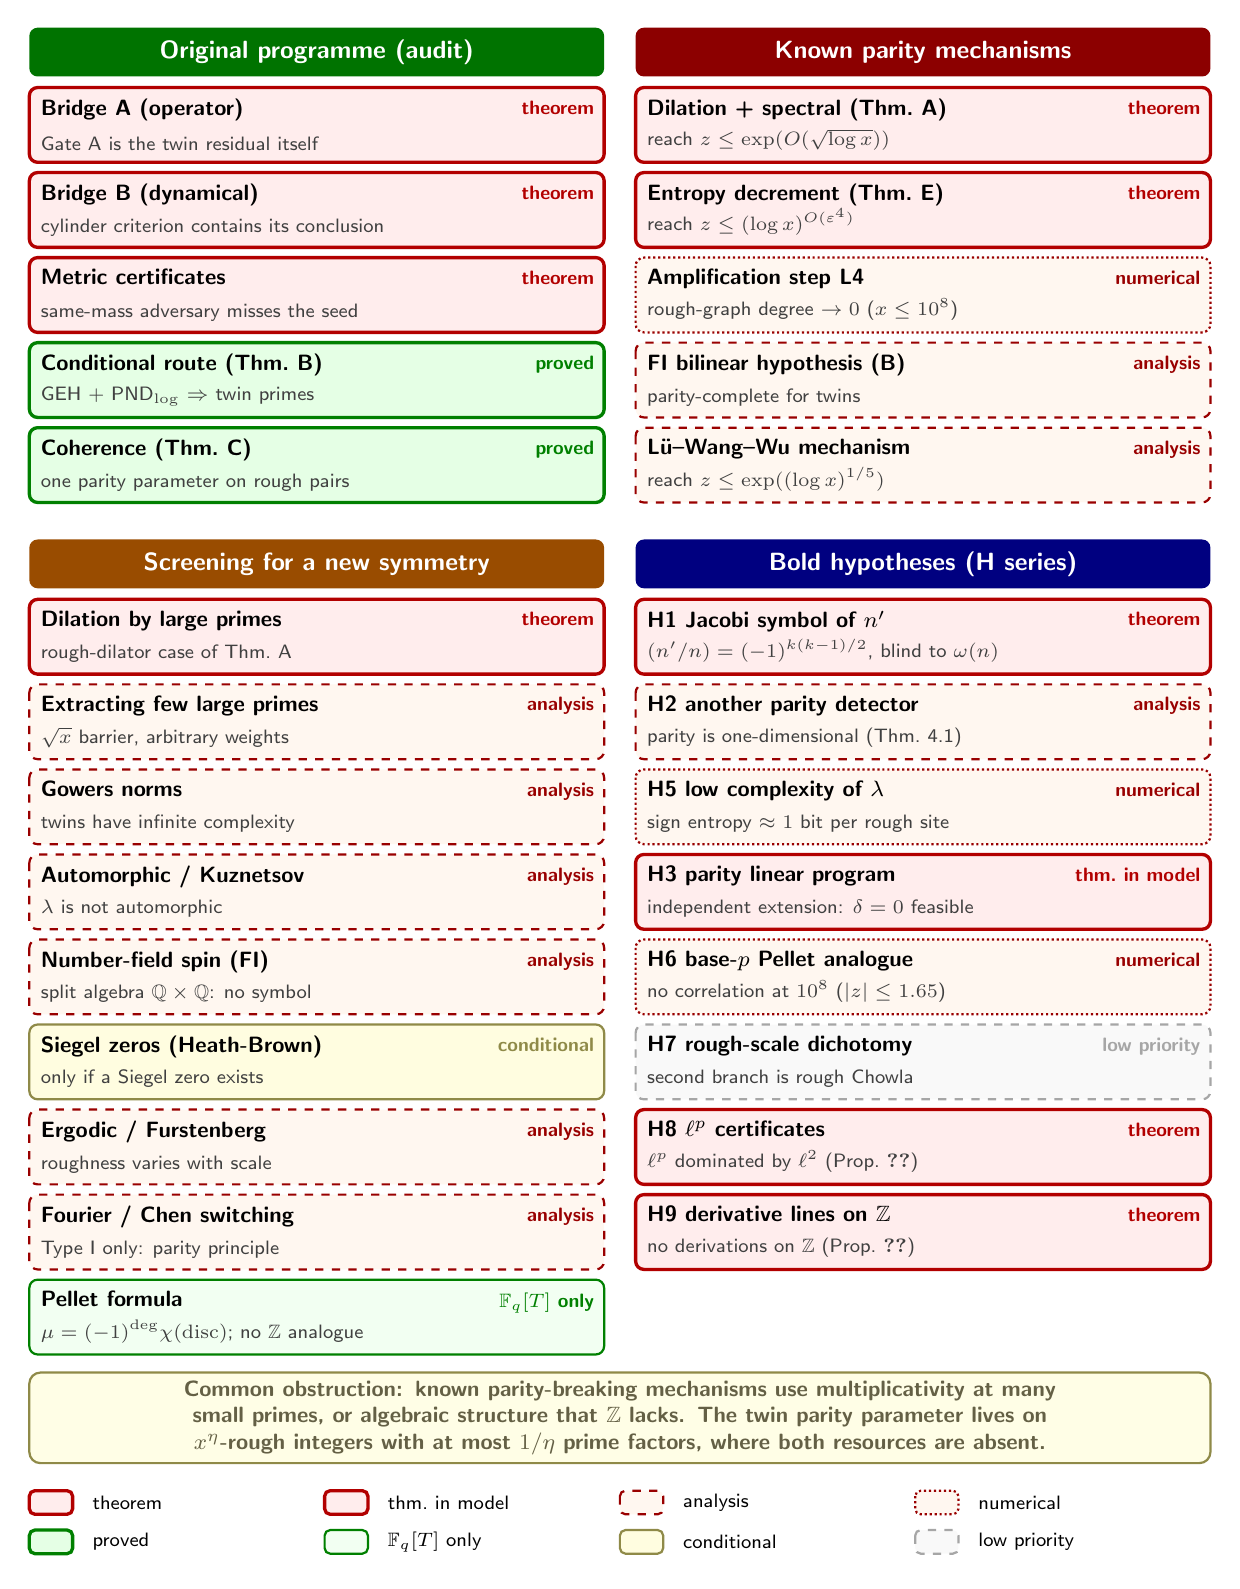
\begin{tikzpicture}[font=\sffamily]
\node[fill=green!45!black, text=white, minimum width=7.3cm, minimum height=0.62cm, inner xsep=0pt, outer sep=0pt, rounded corners=3pt, font=\small\bfseries\sffamily] at (3.650,0.450) {Original programme (audit)};
\draw[very thick, draw=red!70!black, fill=red!7, rounded corners=3pt] (0.000,0.000) rectangle (7.300,-0.950);
\node[anchor=north west, font=\footnotesize\bfseries\sffamily, inner sep=0pt] at (0.140,-0.140) {Bridge A (operator)};
\node[anchor=north east, font=\scriptsize\bfseries\sffamily, text=red!70!black, inner sep=0pt] at (7.180,-0.160) {theorem};
\node[anchor=south west, font=\scriptsize\sffamily, text=black!75, inner sep=0pt] at (0.140,-0.810) {Gate A is the twin residual itself};
\draw[very thick, draw=red!70!black, fill=red!7, rounded corners=3pt] (0.000,-1.080) rectangle (7.300,-2.030);
\node[anchor=north west, font=\footnotesize\bfseries\sffamily, inner sep=0pt] at (0.140,-1.220) {Bridge B (dynamical)};
\node[anchor=north east, font=\scriptsize\bfseries\sffamily, text=red!70!black, inner sep=0pt] at (7.180,-1.240) {theorem};
\node[anchor=south west, font=\scriptsize\sffamily, text=black!75, inner sep=0pt] at (0.140,-1.890) {cylinder criterion contains its conclusion};
\draw[very thick, draw=red!70!black, fill=red!7, rounded corners=3pt] (0.000,-2.160) rectangle (7.300,-3.110);
\node[anchor=north west, font=\footnotesize\bfseries\sffamily, inner sep=0pt] at (0.140,-2.300) {Metric certificates};
\node[anchor=north east, font=\scriptsize\bfseries\sffamily, text=red!70!black, inner sep=0pt] at (7.180,-2.320) {theorem};
\node[anchor=south west, font=\scriptsize\sffamily, text=black!75, inner sep=0pt] at (0.140,-2.970) {same-mass adversary misses the seed};
\draw[very thick, draw=green!50!black, fill=green!10, rounded corners=3pt] (0.000,-3.240) rectangle (7.300,-4.190);
\node[anchor=north west, font=\footnotesize\bfseries\sffamily, inner sep=0pt] at (0.140,-3.380) {Conditional route (Thm.~B)};
\node[anchor=north east, font=\scriptsize\bfseries\sffamily, text=green!50!black, inner sep=0pt] at (7.180,-3.400) {proved};
\node[anchor=south west, font=\scriptsize\sffamily, text=black!75, inner sep=0pt] at (0.140,-4.050) {GEH + PND$_{\log}$ $\Rightarrow$ twin primes};
\draw[very thick, draw=green!50!black, fill=green!10, rounded corners=3pt] (0.000,-4.320) rectangle (7.300,-5.270);
\node[anchor=north west, font=\footnotesize\bfseries\sffamily, inner sep=0pt] at (0.140,-4.460) {Coherence (Thm.~C)};
\node[anchor=north east, font=\scriptsize\bfseries\sffamily, text=green!50!black, inner sep=0pt] at (7.180,-4.480) {proved};
\node[anchor=south west, font=\scriptsize\sffamily, text=black!75, inner sep=0pt] at (0.140,-5.130) {one parity parameter on rough pairs};
\node[fill=red!55!black, text=white, minimum width=7.3cm, minimum height=0.62cm, inner xsep=0pt, outer sep=0pt, rounded corners=3pt, font=\small\bfseries\sffamily] at (11.350,0.450) {Known parity mechanisms};
\draw[very thick, draw=red!70!black, fill=red!7, rounded corners=3pt] (7.700,0.000) rectangle (15.000,-0.950);
\node[anchor=north west, font=\footnotesize\bfseries\sffamily, inner sep=0pt] at (7.840,-0.140) {Dilation + spectral (Thm.~A)};
\node[anchor=north east, font=\scriptsize\bfseries\sffamily, text=red!70!black, inner sep=0pt] at (14.880,-0.160) {theorem};
\node[anchor=south west, font=\scriptsize\sffamily, text=black!75, inner sep=0pt] at (7.840,-0.810) {reach $z\le\exp(O(\sqrt{\log x}))$};
\draw[very thick, draw=red!70!black, fill=red!7, rounded corners=3pt] (7.700,-1.080) rectangle (15.000,-2.030);
\node[anchor=north west, font=\footnotesize\bfseries\sffamily, inner sep=0pt] at (7.840,-1.220) {Entropy decrement (Thm.~E)};
\node[anchor=north east, font=\scriptsize\bfseries\sffamily, text=red!70!black, inner sep=0pt] at (14.880,-1.240) {theorem};
\node[anchor=south west, font=\scriptsize\sffamily, text=black!75, inner sep=0pt] at (7.840,-1.890) {reach $z\le(\log x)^{O(\varepsilon^4)}$};
\draw[thick, densely dotted, draw=red!60!black, fill=orange!6, rounded corners=3pt] (7.700,-2.160) rectangle (15.000,-3.110);
\node[anchor=north west, font=\footnotesize\bfseries\sffamily, inner sep=0pt] at (7.840,-2.300) {Amplification step L4};
\node[anchor=north east, font=\scriptsize\bfseries\sffamily, text=red!60!black, inner sep=0pt] at (14.880,-2.320) {numerical};
\node[anchor=south west, font=\scriptsize\sffamily, text=black!75, inner sep=0pt] at (7.840,-2.970) {rough-graph degree $\to0$ ($x\le10^8$)};
\draw[thick, dashed, draw=red!60!black, fill=orange!6, rounded corners=3pt] (7.700,-3.240) rectangle (15.000,-4.190);
\node[anchor=north west, font=\footnotesize\bfseries\sffamily, inner sep=0pt] at (7.840,-3.380) {FI bilinear hypothesis (B)};
\node[anchor=north east, font=\scriptsize\bfseries\sffamily, text=red!60!black, inner sep=0pt] at (14.880,-3.400) {analysis};
\node[anchor=south west, font=\scriptsize\sffamily, text=black!75, inner sep=0pt] at (7.840,-4.050) {parity-complete for twins};
\draw[thick, dashed, draw=red!60!black, fill=orange!6, rounded corners=3pt] (7.700,-4.320) rectangle (15.000,-5.270);
\node[anchor=north west, font=\footnotesize\bfseries\sffamily, inner sep=0pt] at (7.840,-4.460) {L\"u--Wang--Wu mechanism};
\node[anchor=north east, font=\scriptsize\bfseries\sffamily, text=red!60!black, inner sep=0pt] at (14.880,-4.480) {analysis};
\node[anchor=south west, font=\scriptsize\sffamily, text=black!75, inner sep=0pt] at (7.840,-5.130) {reach $z\le\exp((\log x)^{1/5})$};
\node[fill=orange!60!black, text=white, minimum width=7.3cm, minimum height=0.62cm, inner xsep=0pt, outer sep=0pt, rounded corners=3pt, font=\small\bfseries\sffamily] at (3.650,-6.050) {Screening for a new symmetry};
\draw[very thick, draw=red!70!black, fill=red!7, rounded corners=3pt] (0.000,-6.500) rectangle (7.300,-7.450);
\node[anchor=north west, font=\footnotesize\bfseries\sffamily, inner sep=0pt] at (0.140,-6.640) {Dilation by large primes};
\node[anchor=north east, font=\scriptsize\bfseries\sffamily, text=red!70!black, inner sep=0pt] at (7.180,-6.660) {theorem};
\node[anchor=south west, font=\scriptsize\sffamily, text=black!75, inner sep=0pt] at (0.140,-7.310) {rough-dilator case of Thm.~A};
\draw[thick, dashed, draw=red!60!black, fill=orange!6, rounded corners=3pt] (0.000,-7.580) rectangle (7.300,-8.530);
\node[anchor=north west, font=\footnotesize\bfseries\sffamily, inner sep=0pt] at (0.140,-7.720) {Extracting few large primes};
\node[anchor=north east, font=\scriptsize\bfseries\sffamily, text=red!60!black, inner sep=0pt] at (7.180,-7.740) {analysis};
\node[anchor=south west, font=\scriptsize\sffamily, text=black!75, inner sep=0pt] at (0.140,-8.390) {$\sqrt x$ barrier, arbitrary weights};
\draw[thick, dashed, draw=red!60!black, fill=orange!6, rounded corners=3pt] (0.000,-8.660) rectangle (7.300,-9.610);
\node[anchor=north west, font=\footnotesize\bfseries\sffamily, inner sep=0pt] at (0.140,-8.800) {Gowers norms};
\node[anchor=north east, font=\scriptsize\bfseries\sffamily, text=red!60!black, inner sep=0pt] at (7.180,-8.820) {analysis};
\node[anchor=south west, font=\scriptsize\sffamily, text=black!75, inner sep=0pt] at (0.140,-9.470) {twins have infinite complexity};
\draw[thick, dashed, draw=red!60!black, fill=orange!6, rounded corners=3pt] (0.000,-9.740) rectangle (7.300,-10.690);
\node[anchor=north west, font=\footnotesize\bfseries\sffamily, inner sep=0pt] at (0.140,-9.880) {Automorphic / Kuznetsov};
\node[anchor=north east, font=\scriptsize\bfseries\sffamily, text=red!60!black, inner sep=0pt] at (7.180,-9.900) {analysis};
\node[anchor=south west, font=\scriptsize\sffamily, text=black!75, inner sep=0pt] at (0.140,-10.550) {$\lambda$ is not automorphic};
\draw[thick, dashed, draw=red!60!black, fill=orange!6, rounded corners=3pt] (0.000,-10.820) rectangle (7.300,-11.770);
\node[anchor=north west, font=\footnotesize\bfseries\sffamily, inner sep=0pt] at (0.140,-10.960) {Number-field spin (FI)};
\node[anchor=north east, font=\scriptsize\bfseries\sffamily, text=red!60!black, inner sep=0pt] at (7.180,-10.980) {analysis};
\node[anchor=south west, font=\scriptsize\sffamily, text=black!75, inner sep=0pt] at (0.140,-11.630) {split algebra $\mathbb Q\times\mathbb Q$: no symbol};
\draw[thick, draw=yellow!50!black, fill=yellow!12, rounded corners=3pt] (0.000,-11.900) rectangle (7.300,-12.850);
\node[anchor=north west, font=\footnotesize\bfseries\sffamily, inner sep=0pt] at (0.140,-12.040) {Siegel zeros (Heath-Brown)};
\node[anchor=north east, font=\scriptsize\bfseries\sffamily, text=yellow!50!black, inner sep=0pt] at (7.180,-12.060) {conditional};
\node[anchor=south west, font=\scriptsize\sffamily, text=black!75, inner sep=0pt] at (0.140,-12.710) {only if a Siegel zero exists};
\draw[thick, dashed, draw=red!60!black, fill=orange!6, rounded corners=3pt] (0.000,-12.980) rectangle (7.300,-13.930);
\node[anchor=north west, font=\footnotesize\bfseries\sffamily, inner sep=0pt] at (0.140,-13.120) {Ergodic / Furstenberg};
\node[anchor=north east, font=\scriptsize\bfseries\sffamily, text=red!60!black, inner sep=0pt] at (7.180,-13.140) {analysis};
\node[anchor=south west, font=\scriptsize\sffamily, text=black!75, inner sep=0pt] at (0.140,-13.790) {roughness varies with scale};
\draw[thick, dashed, draw=red!60!black, fill=orange!6, rounded corners=3pt] (0.000,-14.060) rectangle (7.300,-15.010);
\node[anchor=north west, font=\footnotesize\bfseries\sffamily, inner sep=0pt] at (0.140,-14.200) {Fourier / Chen switching};
\node[anchor=north east, font=\scriptsize\bfseries\sffamily, text=red!60!black, inner sep=0pt] at (7.180,-14.220) {analysis};
\node[anchor=south west, font=\scriptsize\sffamily, text=black!75, inner sep=0pt] at (0.140,-14.870) {Type I only: parity principle};
\draw[thick, draw=green!50!black, fill=green!5, rounded corners=3pt] (0.000,-15.140) rectangle (7.300,-16.090);
\node[anchor=north west, font=\footnotesize\bfseries\sffamily, inner sep=0pt] at (0.140,-15.280) {Pellet formula};
\node[anchor=north east, font=\scriptsize\bfseries\sffamily, text=green!50!black, inner sep=0pt] at (7.180,-15.300) {$\mathbb F_q[T]$ only};
\node[anchor=south west, font=\scriptsize\sffamily, text=black!75, inner sep=0pt] at (0.140,-15.950) {$\mu=(-1)^{\deg}\chi(\operatorname{disc})$; no $\mathbb Z$ analogue};
\node[fill=blue!50!black, text=white, minimum width=7.3cm, minimum height=0.62cm, inner xsep=0pt, outer sep=0pt, rounded corners=3pt, font=\small\bfseries\sffamily] at (11.350,-6.050) {Bold hypotheses (H series)};
\draw[very thick, draw=red!70!black, fill=red!7, rounded corners=3pt] (7.700,-6.500) rectangle (15.000,-7.450);
\node[anchor=north west, font=\footnotesize\bfseries\sffamily, inner sep=0pt] at (7.840,-6.640) {H1 Jacobi symbol of $n'$};
\node[anchor=north east, font=\scriptsize\bfseries\sffamily, text=red!70!black, inner sep=0pt] at (14.880,-6.660) {theorem};
\node[anchor=south west, font=\scriptsize\sffamily, text=black!75, inner sep=0pt] at (7.840,-7.310) {$(n'/n)=(-1)^{k(k-1)/2}$, blind to $\omega(n)$};
\draw[thick, dashed, draw=red!60!black, fill=orange!6, rounded corners=3pt] (7.700,-7.580) rectangle (15.000,-8.530);
\node[anchor=north west, font=\footnotesize\bfseries\sffamily, inner sep=0pt] at (7.840,-7.720) {H2 another parity detector};
\node[anchor=north east, font=\scriptsize\bfseries\sffamily, text=red!60!black, inner sep=0pt] at (14.880,-7.740) {analysis};
\node[anchor=south west, font=\scriptsize\sffamily, text=black!75, inner sep=0pt] at (7.840,-8.390) {parity is one-dimensional (Thm.~4.1)};
\draw[thick, densely dotted, draw=red!60!black, fill=orange!6, rounded corners=3pt] (7.700,-8.660) rectangle (15.000,-9.610);
\node[anchor=north west, font=\footnotesize\bfseries\sffamily, inner sep=0pt] at (7.840,-8.800) {H5 low complexity of $\lambda$};
\node[anchor=north east, font=\scriptsize\bfseries\sffamily, text=red!60!black, inner sep=0pt] at (14.880,-8.820) {numerical};
\node[anchor=south west, font=\scriptsize\sffamily, text=black!75, inner sep=0pt] at (7.840,-9.470) {sign entropy $\approx1$ bit per rough site};
\draw[very thick, draw=red!70!black, fill=red!7, rounded corners=3pt] (7.700,-9.740) rectangle (15.000,-10.690);
\node[anchor=north west, font=\footnotesize\bfseries\sffamily, inner sep=0pt] at (7.840,-9.880) {H3 parity linear program};
\node[anchor=north east, font=\scriptsize\bfseries\sffamily, text=red!70!black, inner sep=0pt] at (14.880,-9.900) {thm.\ in model};
\node[anchor=south west, font=\scriptsize\sffamily, text=black!75, inner sep=0pt] at (7.840,-10.550) {independent extension: $\delta=0$ feasible};
\draw[thick, densely dotted, draw=red!60!black, fill=orange!6, rounded corners=3pt] (7.700,-10.820) rectangle (15.000,-11.770);
\node[anchor=north west, font=\footnotesize\bfseries\sffamily, inner sep=0pt] at (7.840,-10.960) {H6 base-$p$ Pellet analogue};
\node[anchor=north east, font=\scriptsize\bfseries\sffamily, text=red!60!black, inner sep=0pt] at (14.880,-10.980) {numerical};
\node[anchor=south west, font=\scriptsize\sffamily, text=black!75, inner sep=0pt] at (7.840,-11.630) {no correlation at $10^8$ ($|z|\le1.65$)};
\draw[thick, dashed, draw=gray!70, fill=gray!5, rounded corners=3pt] (7.700,-11.900) rectangle (15.000,-12.850);
\node[anchor=north west, font=\footnotesize\bfseries\sffamily, inner sep=0pt] at (7.840,-12.040) {H7 rough-scale dichotomy};
\node[anchor=north east, font=\scriptsize\bfseries\sffamily, text=gray!70, inner sep=0pt] at (14.880,-12.060) {low priority};
\node[anchor=south west, font=\scriptsize\sffamily, text=black!75, inner sep=0pt] at (7.840,-12.710) {second branch is rough Chowla};
\draw[very thick, draw=red!70!black, fill=red!7, rounded corners=3pt] (7.700,-12.980) rectangle (15.000,-13.930);
\node[anchor=north west, font=\footnotesize\bfseries\sffamily, inner sep=0pt] at (7.840,-13.120) {H8 $\ell^p$ certificates};
\node[anchor=north east, font=\scriptsize\bfseries\sffamily, text=red!70!black, inner sep=0pt] at (14.880,-13.140) {theorem};
\node[anchor=south west, font=\scriptsize\sffamily, text=black!75, inner sep=0pt] at (7.840,-13.790) {$\ell^p$ dominated by $\ell^2$ (Prop.~\ref{prop:L})};
\draw[very thick, draw=red!70!black, fill=red!7, rounded corners=3pt] (7.700,-14.060) rectangle (15.000,-15.010);
\node[anchor=north west, font=\footnotesize\bfseries\sffamily, inner sep=0pt] at (7.840,-14.200) {H9 derivative lines on $\mathbb Z$};
\node[anchor=north east, font=\scriptsize\bfseries\sffamily, text=red!70!black, inner sep=0pt] at (14.880,-14.220) {theorem};
\node[anchor=south west, font=\scriptsize\sffamily, text=black!75, inner sep=0pt] at (7.840,-14.870) {no derivations on $\mathbb Z$ (Prop.~\ref{prop:noderiv})};
\draw[thick, draw=yellow!50!black, fill=yellow!10, rounded corners=4pt] (0,-16.320) rectangle (15.000,-17.470);
\node[align=center, text width=14.60cm, font=\footnotesize\bfseries\sffamily, text=yellow!30!black] at (7.500,-16.895) {Common obstruction: known parity-breaking mechanisms use multiplicativity at many small primes, or algebraic structure that $\mathbb Z$ lacks. The twin parity parameter lives on $x^\eta$-rough integers with at most $1/\eta$ prime factors, where both resources are absent.};
\draw[very thick, draw=red!70!black, fill=red!7, rounded corners=2pt] (0.000,-17.820) rectangle (0.550,-18.120);
\node[anchor=west, font=\scriptsize\sffamily] at (0.680,-17.970) {theorem};
\draw[very thick, draw=red!70!black, fill=red!7, rounded corners=2pt] (3.750,-17.820) rectangle (4.300,-18.120);
\node[anchor=west, font=\scriptsize\sffamily] at (4.430,-17.970) {thm.\ in model};
\draw[thick, dashed, draw=red!60!black, fill=orange!6, rounded corners=2pt] (7.500,-17.820) rectangle (8.050,-18.120);
\node[anchor=west, font=\scriptsize\sffamily] at (8.180,-17.970) {analysis};
\draw[thick, densely dotted, draw=red!60!black, fill=orange!6, rounded corners=2pt] (11.250,-17.820) rectangle (11.800,-18.120);
\node[anchor=west, font=\scriptsize\sffamily] at (11.930,-17.970) {numerical};
\draw[very thick, draw=green!50!black, fill=green!10, rounded corners=2pt] (0.000,-18.320) rectangle (0.550,-18.620);
\node[anchor=west, font=\scriptsize\sffamily] at (0.680,-18.470) {proved};
\draw[thick, draw=green!50!black, fill=green!5, rounded corners=2pt] (3.750,-18.320) rectangle (4.300,-18.620);
\node[anchor=west, font=\scriptsize\sffamily] at (4.430,-18.470) {$\mathbb F_q[T]$ only};
\draw[thick, draw=yellow!50!black, fill=yellow!12, rounded corners=2pt] (7.500,-18.320) rectangle (8.050,-18.620);
\node[anchor=west, font=\scriptsize\sffamily] at (8.180,-18.470) {conditional};
\draw[thick, dashed, draw=gray!70, fill=gray!5, rounded corners=2pt] (11.250,-18.320) rectangle (11.800,-18.620);
\node[anchor=west, font=\scriptsize\sffamily] at (11.930,-18.470) {low priority};
\end{tikzpicture}}
\caption{Map of every route explored in this project, with its status. ``Theorem'' means a complete proof in this paper or in the separate audit of the original programme (first column); ``thm.\ in model'' means an explicit construction that is rigorous within the stated model; ``analysis'' and ``numerical'' are judgements about specific arguments or data, not theorems. All entries were obtained with AI assistance and have not yet been checked by a specialist (Appendix~\ref{app:ai}).}
\label{fig:exploration}
\end{figure}


\paragraph{The Friedlander--Iwaniec bilinear hypothesis.} In the asymptotic sieve for primes \cite{FI98}, parity is broken by a bilinear hypothesis (B). For the twin sequence $a_k=\mathbf 1_{\mathbb P}(k+2)$ it reads
\[
\sum_m\Bigl|\sum_{N<n\le2N}\gamma(n,C)\mu(n)\mathbf 1_{\mathbb P}(mn+2)\Bigr|=o\Bigl(\frac{x}{\log x}\Bigr)
\]
for every $N$ in a range that always contains $N\approx\sqrt x$, with arbitrary coefficients on $m$ because of the absolute values. We tried three ways of reducing (B) to known estimates; each ends in an obstruction:
\begin{itemize}
\item a Heath-Brown decomposition of $\Lambda(mn+2)$ leaves a determinant sum over $mn-de=-2$ with Möbius-type coefficients on both sides, which is two-point Chowla on a determinant variety;
\item extracting small primes from the unshifted variable $n$, in the manner of \cite{LWW26}, removes $\mu$ but squares the prime side into a binary prime correlation, with coefficients larger than the range of the variable;
\item Cauchy--Schwarz in $m$ returns the $L^2$ form of (B) itself.
\end{itemize}
Beyond $\sqrt x$, distribution results with arbitrary coefficients are not known. We call (B) \emph{parity-complete} for twins: this is an analysis of known techniques, not an impossibility statement.

\paragraph{Screening for a new symmetry.} We tested nine classes of mechanisms against three criteria: (i) they must act on $x^\eta$-rough integers without extracting small primes; (ii) they must be parity-sensitive; (iii) they must not be blocked by a known obstruction. Only Pellet's formula $\mu(f)=(-1)^{\deg f}\chi(\operatorname{disc}f)$ over $\mathbb F_q[T]$ passes, and it is the mechanism behind the function-field twin prime theorem of Sawin and Shusterman \cite{SS22}. We verified it for all squarefree monic polynomials over $\mathbb F_3$ (degree $\le7$) and $\mathbb F_5$ (degree $\le5$), including those whose smallest irreducible factor has large degree. The reason it has no integer analogue is that, for fixed degree, $\mu$ on $\mathbb F_q[T]$ is a quadratic character of a polynomial in the coefficients, which Weil--Deligne estimates can control. No comparable structure is known for $\lambda$ on $\mathbb Z$.

\paragraph{The H series.} Table~\ref{tab:hledger} lists the bold hypotheses and their fate.

\begin{table}[H]
\centering
\small
\begin{tabular}{p{3.4cm}p{1.6cm}p{7.4cm}}
\toprule
hypothesis & status & reason\\
\midrule
H1: the Jacobi symbol of the arithmetic derivative $n'=\sum_{p\mid n}n/p$ detects $(-1)^{\omega(n)}$ & false (proof) & For odd squarefree $n$, quadratic reciprocity gives $(n'/n)=(-1)^{k(k-1)/2}$ with $k=\#\{p\mid n:p\equiv3\bmod4\}$, so the symbol is blind to $\omega(n)$. Checked for all $81{,}053$ cases $n\le2\cdot10^5$; agreement with $\lambda$ is $0.4935$.\\
H2: a different parity detector is easier to control & false (analysis) & By Theorem~\ref{thm:onesided}, every detector separating primes from $P_2$ is governed by the same parameter $\delta$.\\
H3: positivity across many patterns forces $\delta_{\rm twin}>0$ & false (model) & A linear program with patterns of $3$ and $4$ shifts, up to $966$ variables, gives $\delta_{\rm twin}\in[0,2]$ in every case. Explicit witness: the extreme counterfeit on $(n,n+2)$, extended independently to all other entries.\\
H5: $\lambda$ has low complexity on rough integers & false (numerical) & The sign entropy is about $1$ bit per rough site up to $x=10^8$.\\
H6: $\lambda(n)$ correlates with the function-field Möbius of the base-$p$ digit polynomial of $n$ & false (numerical) & With $p=463$ ($d=2$) and $p=97$ ($d=3$), about $10^8$ integers each, all twelve correlations (for $\lambda$, $\mu$ and rough $\lambda$) are within noise, $|z|\le1.65$, so $|\mathrm{corr}|\lesssim3\cdot10^{-4}$.\\
H7: a Heath-Brown type dichotomy at rough scale & open (low priority) & Its second branch is the Chowla conjecture on rough integers.\\
H9: $\lambda$ is a Dirichlet character on a positive-density family of integer ``lines'', as $\mu$ is in $\mathbb F_q[T]$ & false (proof and numerical) & There are no derivations on $\mathbb Z$, local substitutes give periodic functions, and permutation-sign discriminants are Jacobi symbols (Proposition~\ref{prop:noderiv}). Line-dependent large-conductor Jacobi symbols: twelve tests at $x=10^8$ within noise, planted control $z\approx800$ (Remark~\ref{rem:H9}).\\
H10--H16: techniques from 2026 AI-generated papers (bounded independence, prime-slot Type~II, zero-free regions, exclusion of Siegel zeros, weighted vertices, Hardy--Littlewood--Chowla transfer, dictionary search) give parity on rough pairs & false (analysis and numerical) & Each takes its sign from small primes or gives no bound beyond $0\le\delta\le2$; numerical cards null at $x=10^8$ with controls at $z\approx565$--$811$. Weighted vertices led to the improved Proposition~\ref{prop:T}.\\
H17--H23: structure for $\sum a_mb_n\lambda(mn+2)$ (dispersion, low rank, norm forms, entropy decrement in a prime variable, small characters, residue forcing, Mellin) & false (analysis and numerical) & Remark~\ref{rem:cards}; the Mellin test led to the absolute-value barrier of Remark~\ref{rem:mellin}.\\
H8: $\ell^p$ or weighted $\ell^2$ certificates pass the $t$-ceiling of Proposition~\ref{prop:T} & false ($\ell^p$: proof); weighted: numerical & $\ell^p$ certificates are dominated by $\ell^2$ (Proposition~\ref{prop:L}). Weights $|g_t|^\beta$ improve the resolution only by constant factors at $x=10^7$, with no detectable change of exponent.\\
\bottomrule
\end{tabular}
\caption{The hypothesis ledger.}
\label{tab:hledger}
\end{table}

\noindent Two lessons from the ledger are worth recording.
\begin{itemize}
\item In H3, the base mass in the one-sided constraints must be the \emph{actual} mass of the sub-pattern, which is itself a variable. A first hand computation that used the model mass instead appeared to force $\delta\approx1$; that was a false positive.
\item In H6, integer carries make multiplication incompatible with digit polynomials, which is why $\lambda$ and the digit-polynomial Möbius function are unrelated.
\end{itemize}
Every reason recorded above points to the obstruction stated in Remark~\ref{rem:common}.

\subsection{Limitations}
All proofs were drafted and checked within the same AI-assisted process. None has yet been independently checked by a human specialist, and errors of the kind listed above may remain. The following points are the most delicate:
\begin{itemize}
\item the uniform upper bound (U) in Theorem~\ref{thm:onesided};
\item the treatment of boundary boxes in Lemma~\ref{lem:geh-box};
\item conditions (A3)--(A4) of Definition~\ref{def:cert}, in particular whether the rarer exceptional sets of \cite{HR21,Pil23} meet at most half of $\mathcal K$;
\item in Proposition~\ref{prop:T}, the uniformity in $t$ of the Selberg--Delange and Nair--Tenenbaum inputs, which are used as black boxes;
\item in Proposition~\ref{prop:Q}, the axioms for the difference sequence $b$, and the size of $\varepsilon(x)$, which we have not quantified;
\item in Section~\ref{sec:locate}, the census of Table~\ref{tab:census} is not claimed to be exhaustive, Remark~\ref{rem:MRT} is an analysis of one proof, and Proposition~\ref{prop:absbarrier} is proved for the Bohr mean and, by Corollary~\ref{cor:absbarrierT}, for windows $T\gg x^4$, but not for the windows $T\asymp x$ used in practice, and only for prime supports, with a very small constant;
\item Remark~\ref{rem:conjA} comes from a separate AI session and is conditional on Conjecture~A, which is supported only numerically;
\item the 2026 AI-generated preprints cited as \cite{OpenAI26} have not been refereed, and we did not check their proofs;
\item in Proposition~\ref{prop:disjunction}, we rely on the published construction of the weights in \cite{Polymath8b} and have not re-derived Theorems~3.14 and~3.15 there.
\end{itemize}
Bombieri's original paper, Chapter~16 of \cite{FI10}, and \cite{MV17} were not read in full. We would be grateful for corrections.


\bibliographystyle{amsplain}
\bibliography{refs}
\end{document}
